% Options for packages loaded elsewhere
\PassOptionsToPackage{unicode}{hyperref}
\PassOptionsToPackage{hyphens}{url}
%
\documentclass[
  12pt,
]{article}
\usepackage{lmodern}
\usepackage{amssymb,amsmath}
\usepackage{ifxetex,ifluatex}
\ifnum 0\ifxetex 1\fi\ifluatex 1\fi=0 % if pdftex
  \usepackage[T1]{fontenc}
  \usepackage[utf8]{inputenc}
  \usepackage{textcomp} % provide euro and other symbols
\else % if luatex or xetex
  \usepackage{unicode-math}
  \defaultfontfeatures{Scale=MatchLowercase}
  \defaultfontfeatures[\rmfamily]{Ligatures=TeX,Scale=1}
  \setmainfont[]{Times New Roman}
\fi
% Use upquote if available, for straight quotes in verbatim environments
\IfFileExists{upquote.sty}{\usepackage{upquote}}{}
\IfFileExists{microtype.sty}{% use microtype if available
  \usepackage[]{microtype}
  \UseMicrotypeSet[protrusion]{basicmath} % disable protrusion for tt fonts
}{}
\makeatletter
\@ifundefined{KOMAClassName}{% if non-KOMA class
  \IfFileExists{parskip.sty}{%
    \usepackage{parskip}
  }{% else
    \setlength{\parindent}{0pt}
    \setlength{\parskip}{6pt plus 2pt minus 1pt}}
}{% if KOMA class
  \KOMAoptions{parskip=half}}
\makeatother
\usepackage{xcolor}
\IfFileExists{xurl.sty}{\usepackage{xurl}}{} % add URL line breaks if available
\IfFileExists{bookmark.sty}{\usepackage{bookmark}}{\usepackage{hyperref}}
\hypersetup{
  hidelinks,
  pdfcreator={LaTeX via pandoc}}
\urlstyle{same} % disable monospaced font for URLs
\usepackage[margin=25mm]{geometry}
\usepackage{color}
\usepackage{fancyvrb}
\newcommand{\VerbBar}{|}
\newcommand{\VERB}{\Verb[commandchars=\\\{\}]}
\DefineVerbatimEnvironment{Highlighting}{Verbatim}{commandchars=\\\{\}}
% Add ',fontsize=\small' for more characters per line
\usepackage{framed}
\definecolor{shadecolor}{RGB}{248,248,248}
\newenvironment{Shaded}{\begin{snugshade}}{\end{snugshade}}
\newcommand{\AlertTok}[1]{\textcolor[rgb]{0.94,0.16,0.16}{#1}}
\newcommand{\AnnotationTok}[1]{\textcolor[rgb]{0.56,0.35,0.01}{\textbf{\textit{#1}}}}
\newcommand{\AttributeTok}[1]{\textcolor[rgb]{0.77,0.63,0.00}{#1}}
\newcommand{\BaseNTok}[1]{\textcolor[rgb]{0.00,0.00,0.81}{#1}}
\newcommand{\BuiltInTok}[1]{#1}
\newcommand{\CharTok}[1]{\textcolor[rgb]{0.31,0.60,0.02}{#1}}
\newcommand{\CommentTok}[1]{\textcolor[rgb]{0.56,0.35,0.01}{\textit{#1}}}
\newcommand{\CommentVarTok}[1]{\textcolor[rgb]{0.56,0.35,0.01}{\textbf{\textit{#1}}}}
\newcommand{\ConstantTok}[1]{\textcolor[rgb]{0.00,0.00,0.00}{#1}}
\newcommand{\ControlFlowTok}[1]{\textcolor[rgb]{0.13,0.29,0.53}{\textbf{#1}}}
\newcommand{\DataTypeTok}[1]{\textcolor[rgb]{0.13,0.29,0.53}{#1}}
\newcommand{\DecValTok}[1]{\textcolor[rgb]{0.00,0.00,0.81}{#1}}
\newcommand{\DocumentationTok}[1]{\textcolor[rgb]{0.56,0.35,0.01}{\textbf{\textit{#1}}}}
\newcommand{\ErrorTok}[1]{\textcolor[rgb]{0.64,0.00,0.00}{\textbf{#1}}}
\newcommand{\ExtensionTok}[1]{#1}
\newcommand{\FloatTok}[1]{\textcolor[rgb]{0.00,0.00,0.81}{#1}}
\newcommand{\FunctionTok}[1]{\textcolor[rgb]{0.00,0.00,0.00}{#1}}
\newcommand{\ImportTok}[1]{#1}
\newcommand{\InformationTok}[1]{\textcolor[rgb]{0.56,0.35,0.01}{\textbf{\textit{#1}}}}
\newcommand{\KeywordTok}[1]{\textcolor[rgb]{0.13,0.29,0.53}{\textbf{#1}}}
\newcommand{\NormalTok}[1]{#1}
\newcommand{\OperatorTok}[1]{\textcolor[rgb]{0.81,0.36,0.00}{\textbf{#1}}}
\newcommand{\OtherTok}[1]{\textcolor[rgb]{0.56,0.35,0.01}{#1}}
\newcommand{\PreprocessorTok}[1]{\textcolor[rgb]{0.56,0.35,0.01}{\textit{#1}}}
\newcommand{\RegionMarkerTok}[1]{#1}
\newcommand{\SpecialCharTok}[1]{\textcolor[rgb]{0.00,0.00,0.00}{#1}}
\newcommand{\SpecialStringTok}[1]{\textcolor[rgb]{0.31,0.60,0.02}{#1}}
\newcommand{\StringTok}[1]{\textcolor[rgb]{0.31,0.60,0.02}{#1}}
\newcommand{\VariableTok}[1]{\textcolor[rgb]{0.00,0.00,0.00}{#1}}
\newcommand{\VerbatimStringTok}[1]{\textcolor[rgb]{0.31,0.60,0.02}{#1}}
\newcommand{\WarningTok}[1]{\textcolor[rgb]{0.56,0.35,0.01}{\textbf{\textit{#1}}}}
\usepackage{graphicx,grffile}
\makeatletter
\def\maxwidth{\ifdim\Gin@nat@width>\linewidth\linewidth\else\Gin@nat@width\fi}
\def\maxheight{\ifdim\Gin@nat@height>\textheight\textheight\else\Gin@nat@height\fi}
\makeatother
% Scale images if necessary, so that they will not overflow the page
% margins by default, and it is still possible to overwrite the defaults
% using explicit options in \includegraphics[width, height, ...]{}
\setkeys{Gin}{width=\maxwidth,height=\maxheight,keepaspectratio}
% Set default figure placement to htbp
\makeatletter
\def\fps@figure{htbp}
\makeatother
\setlength{\emergencystretch}{3em} % prevent overfull lines
\providecommand{\tightlist}{%
  \setlength{\itemsep}{0pt}\setlength{\parskip}{0pt}}
\setcounter{secnumdepth}{-\maxdimen} % remove section numbering
\usepackage{setspace}
\renewcommand{\contentsname}{\Huge{Table des matières}}
\usepackage{tocloft}

\title{\vspace{5cm}
\textbf{Amélioration de l'accès aux résultats biologiques :}\\
\textbf{Séquençage ARN et Application Shiny}}
\usepackage{etoolbox}
\makeatletter
\providecommand{\subtitle}[1]{% add subtitle to \maketitle
  \apptocmd{\@title}{\par {\large #1 \par}}{}{}
}
\makeatother
\subtitle{Master 1 Bioinformatique\\
Université de Rennes 1\\
2019 - 2020}
\author{\centering 
\includegraphics[width=0.4\textwidth]{logo.png}}
\date{David GALLIEN \& Gabin COUDRAY}

\begin{document}
\maketitle

\textbackslash begin\{document\}

\newpage
\begin{center}
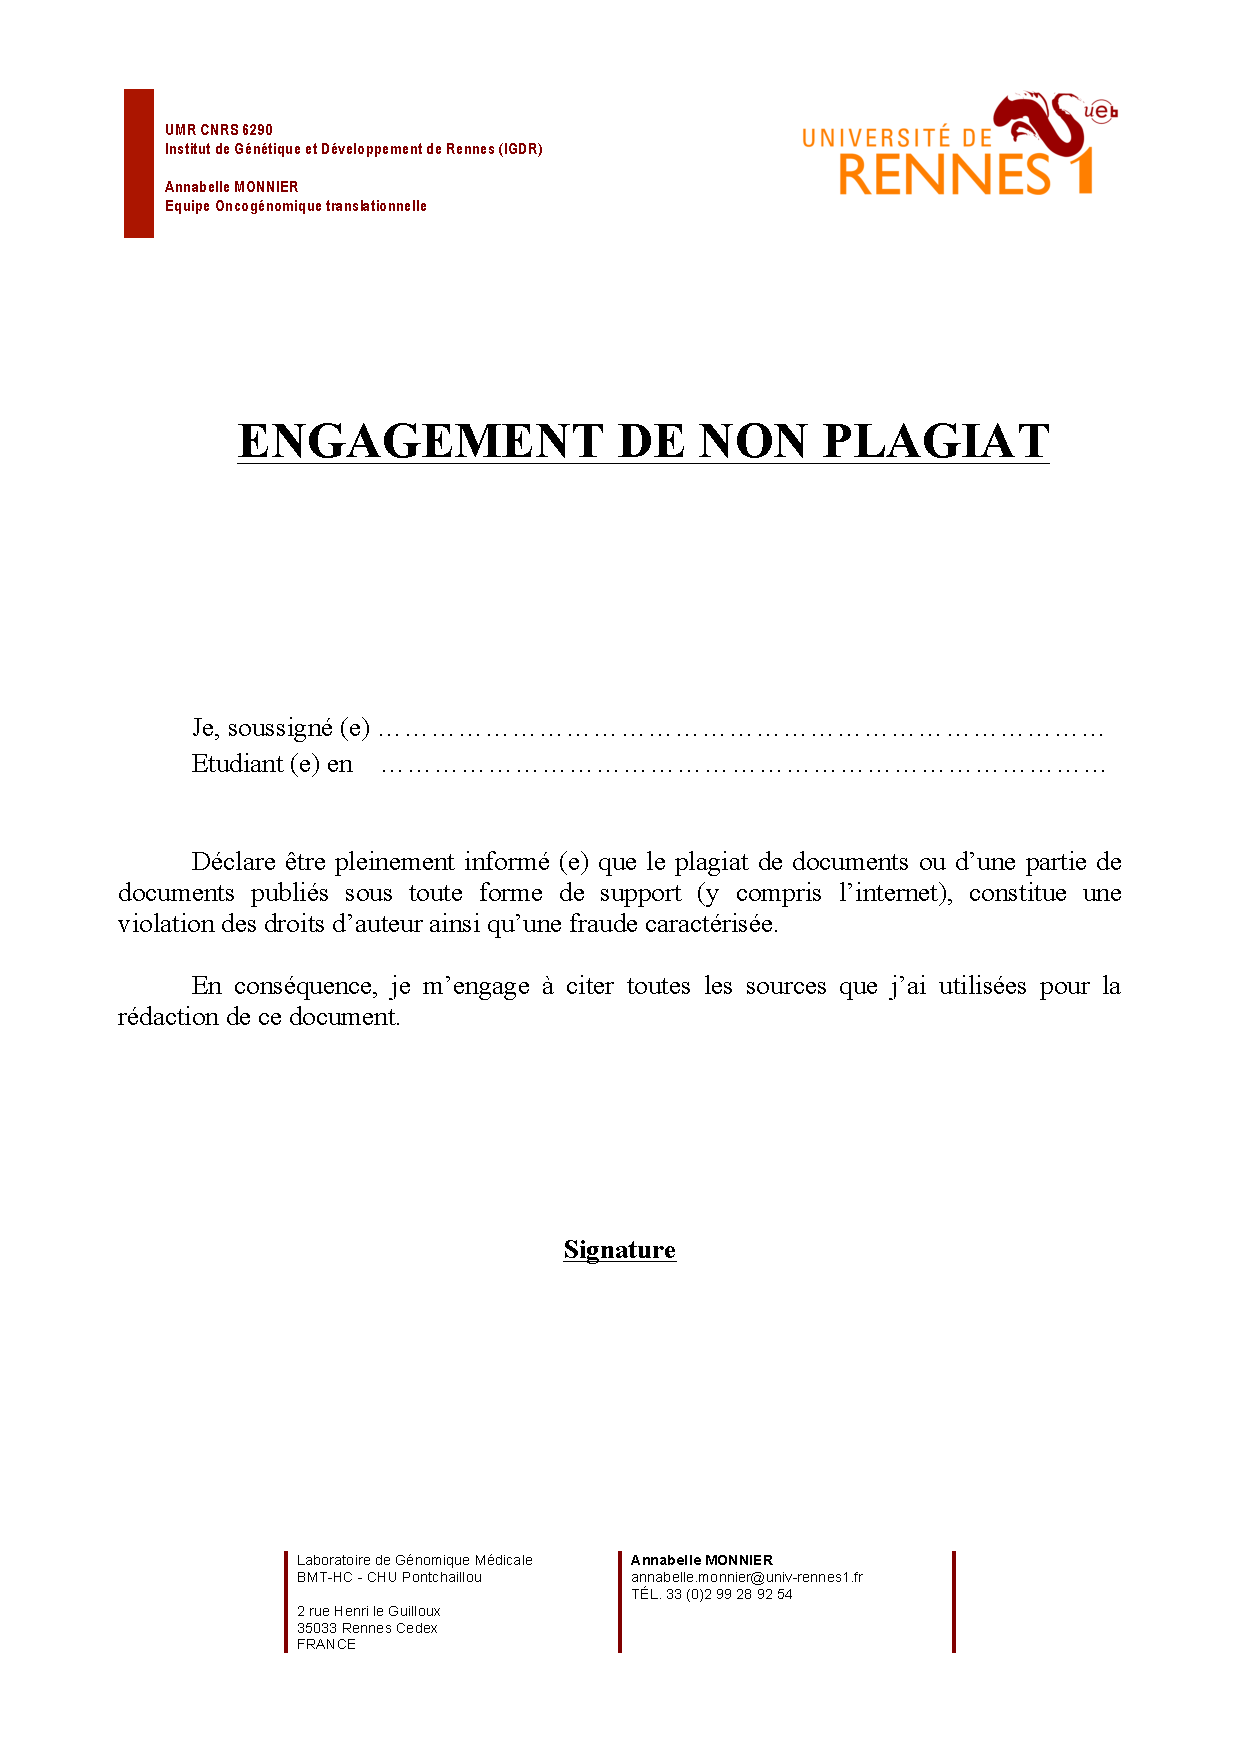
\includegraphics[width=10in]{attestationDeNonPlagiat.pdf}
\end{center}

\newpage
\begin{center}
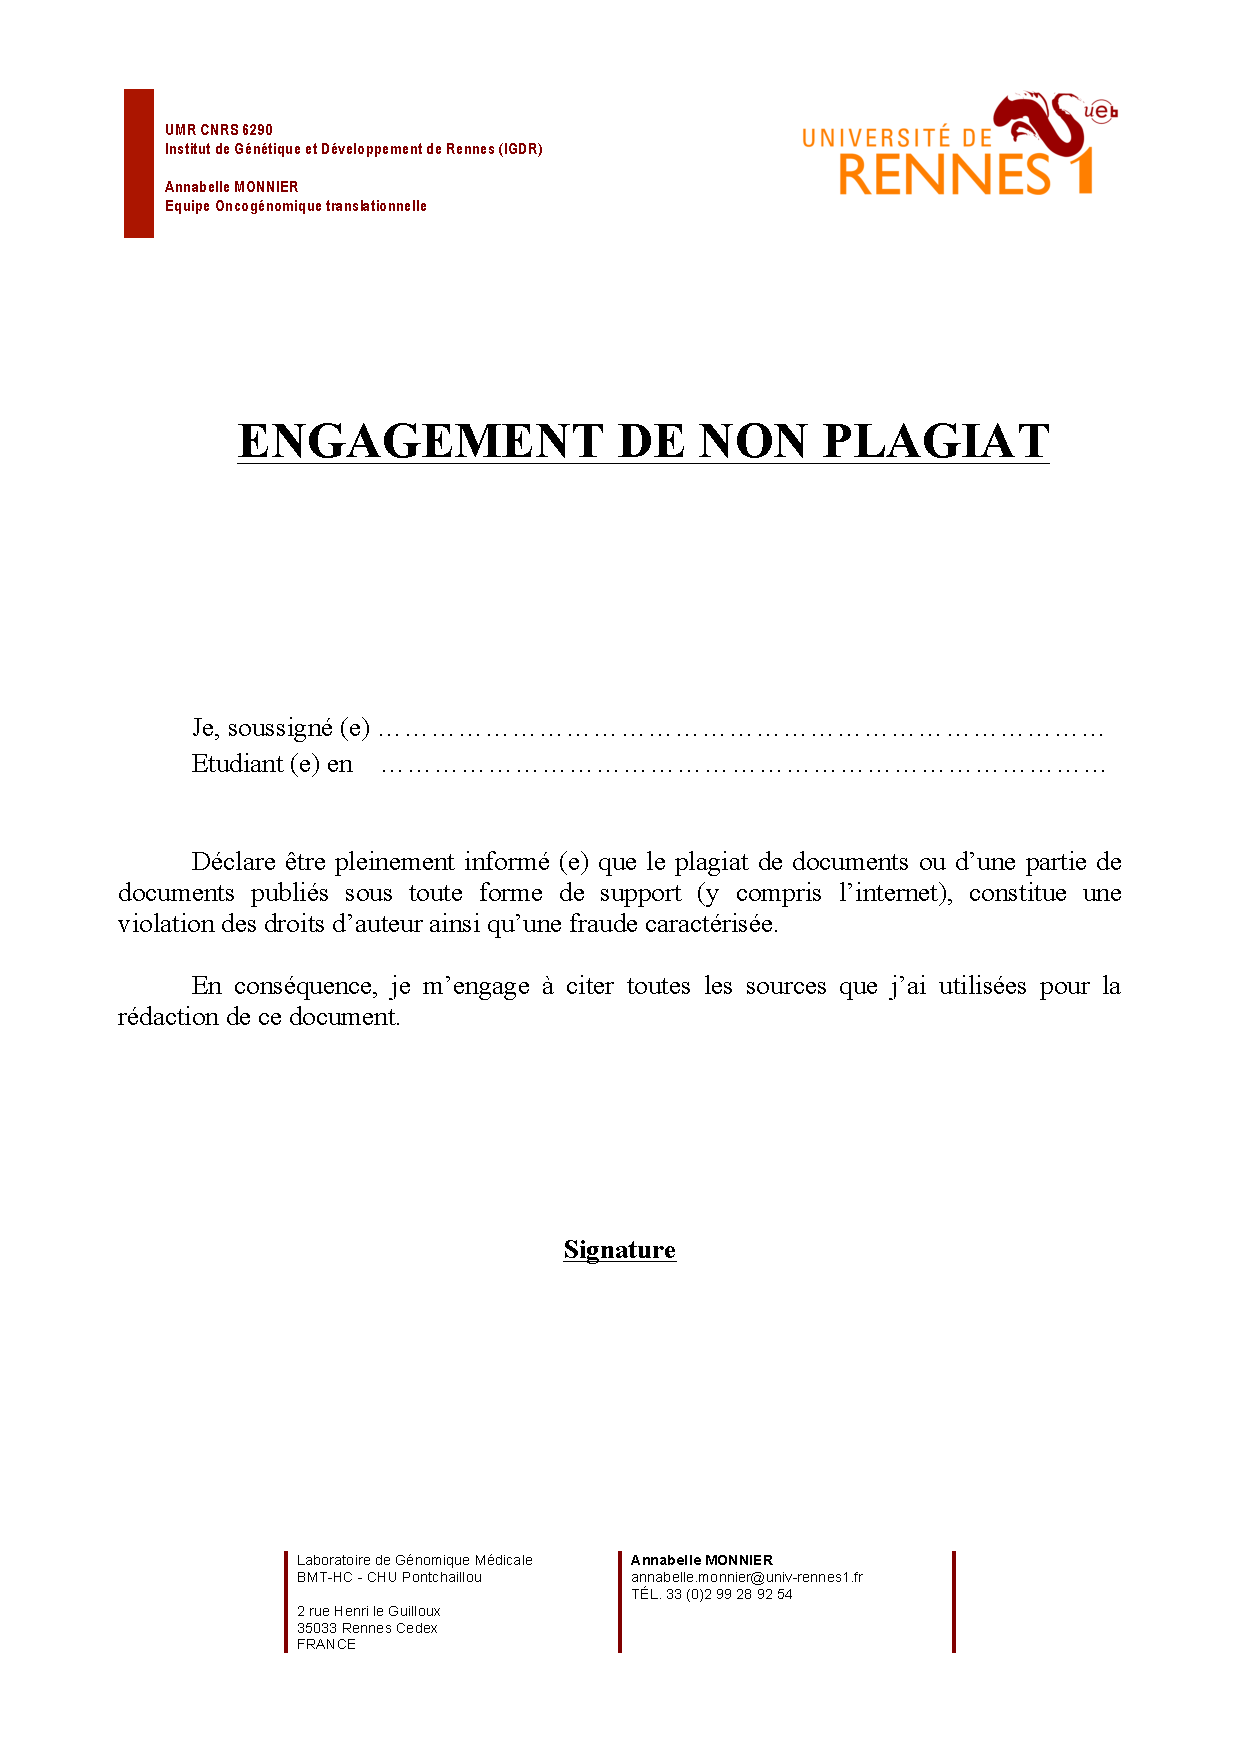
\includegraphics[width=10in]{attestationDeNonPlagiat.pdf}
\end{center}

\setstretch{1.5}

\newpage
\setcounter{tocdepth}{4}
\tableofcontents
\newpage

\hypertarget{introduction}{%
\section{\texorpdfstring{\Large\{Introduction\}}{\{Introduction\}}}\label{introduction}}

\hypertarget{contexte}{%
\subsection{\texorpdfstring{\large\{Contexte\}}{\{Contexte\}}}\label{contexte}}

~~~~~~~ De nos jours, la plupart des chercheurs n'ont en général pas le
temps d'utiliser les outils permettant une analyse des données générées
par les nouvelles technologies. C'est pour cela qu'il est important de
leur offrir la possibilité d'avoir accès à des outils facilitant
l'analyse et leur permettant d'être plus efficaces. Le but principal de
notre projet est de mettre en place une application qui pourra aider ces
scientifiques à explorer leurs résultats sous l'environnement R. Pour
cela le package Shiny nous permet de créer une application web
interactive.

\par

~~~~~~~ Néanmoins, afin de créer une application interactive, nous avons
besoin de quelques choses à montrer. Dans le domaine de la recherche
médicale qui est le principal axe de recherche, les techniques de
séquençage de seconde génération sont souvent utilisées. Ces techniques
génèrent de nombreuses données qui ont besoin d'être explorées et
analysées. Nous avons donc décidé de concentrer notre travail sur le
séquençange de l'ARN (RNA-seq). Cette technique de séquençage de seconde
génération a pour principal but de détecter des expressions
différentielles entre des types cellulaires de différentes conditions.

~~~~~~~ Le RNA-seq est un nouveau moyen permettant un séquençage de
l'ARN plus rapide que les techniques qui existaienet précédemment comme
la méthode de Sanger. Le but principal du RNA-seq est d'étudier
l'expression différentielle de gènes entre différentes conditions. Le
séquançage de l'ARN a été cité pour la première en 2008, et depuis, le
nombre de publication contenant des données de RNA-seq augmentent
d'années en années. Ce genre d'analyses utilises les technologies de
séquançage de nouvelles génération (NGS) comme Illumina, Roche 454 ou
encore Ion Torrent.

Une analyse RNA-seq présente 3 grandes étapes :

\begin{itemize}
\item Fragmentation aléatoire des ARN matures 
\item Amplification de ces fragments par PCR
\item Séquençage de ces fragments donnant des millions de reads
\end{itemize}

~~~~~~~ Le nombre de reads obtenu est proportionnel à l'abondance des
ARN dans la cellules. Ces reads sont stockés dans des fichiers au format
fastQ et leur qualité est estimé grâce à des outils spécifiques.
Ensuite, chaque read est mappé sur le génome de référence de l'organisme
étudié. Après ce mapping, des fichiers BAM sont obtenus. Dans ces
fichiers, chaques ligne représante un alignement d'un read. Pour finir,
un comptage des reads pour chaque position est realisé afin de remplir
une table de comptage permettant l'analyse des données RNA-seq.

\hypertarget{analyse-de-donnuxe9es-rna-seq}{%
\subparagraph{Analyse de données
RNA-seq}\label{analyse-de-donnuxe9es-rna-seq}}

Les étapes de l'analyse RNA-seq présentées ci-dessous sont inspirées du
mode d'emploi d'analyse de données RNA-seq sur le site
\href{https://bioinfo-fr.net/lanalyse-de-donnees-rna-seq-mode-demploi}{\underline{bioinfo-fr.net}}.

\hypertarget{etape-1-les-donnuxe9es}{%
\subparagraph{Etape 1 : Les données}\label{etape-1-les-donnuxe9es}}

Premièrement, pour obtenir le jeu de données, l'ARN est extrait des
cellules et l'ARNm est isolé grâce à sa queue poly-adénylée. Une fois
extrait, l'ARNm est fragmenté et subit une reverse transcription en
ADNc. Ensuite, l'ADNc est séquencé grâce aux NGS. Aujourd'hui, le plus
utilisé est la technologie Illumina qui utilise une amplification
clonale et un séquençage par synthèse. Le séquençage peut être ``single
end'' (chaque read est indépendant) ou ``paired-end'' (les reads sont
pairés). Après le séquençage, des millions de reads sont obtenus.

\hypertarget{etape-2-contruxf4le-qualituxe9}{%
\subparagraph{Etape 2 : Contrôle
qualité}\label{etape-2-contruxf4le-qualituxe9}}

A la sortie du séquenceur on retrouve des fichiers fastQ. Ce genre de
fichier est composé de blocs de 4 lignes représentants un read. Grâce
aux fichiers fastQ, la qualité du séquençage peut être estimée à l'aide
de programmes comme FastQC.

\hypertarget{etape-3-mapping}{%
\subparagraph{Etape 3 : Mapping}\label{etape-3-mapping}}

Cette partie de l'analyse consiste à aligner tous les reads sur le
génome de l'organisme étudié. Un read est mappé sur la régions du génome
qui lui est la plus similaire. Cette étape permet d'obtenir des fichiers
BAM dans lesquels chaque ligne correspond à un read. De plus, la moyenne
du nombre de reads mappés sur une régions est appelée la profondeur.

\hypertarget{etape-4-quantification}{%
\subparagraph{Etape 4 : Quantification}\label{etape-4-quantification}}

Le nombre de reads est un témoin de l'abondance d'ARN dans la cellule.
Ainsi, il est possible d'estimer le niveau d'expression d'un gène. C'est
pourquoi il est important de compter les reads mappés pour chaque gène.
Le but de cette étape est de remplir une table de comptage afin de
pouvoir la manipuler facilement avec R par exemple.

\hypertarget{etape-5-statistiques}{%
\subparagraph{Etape 5 : Statistiques}\label{etape-5-statistiques}}

Différents résultats statistiques peuvent être obtenus ainsi que des
graphiques ou encore des carte de densité pour les exons. Il est
important de normaliser les données et de comparer les p-value ajustées
obtenues après différents tests. Tout ceci permet d'établir une liste de
gène différentiellement exprimés.

\hypertarget{objectifs}{%
\subsection{\texorpdfstring{\large\{Objectifs\}}{\{Objectifs\}}}\label{objectifs}}

~~~~~~~ Aujourd'hui, de plus en plus d'études utilisent le séquençage de
l'ARN, il en résulte de plus en plus de données à analyser. Pour essayer
de répondre à cette problématique nous avons décidé d'élaborer une
application interactive grâce au package RShiny. Cette application a
pour but d'aider à l'analyse de données RNA-seq le plus profondément
possible en répondant aux plus de questions possibles et permettre une
visualisation intuitive des résultats. Le but de ce projet est de nous
permettre d'en apprendre plus sur cette nouvelle technique de séquençage
de l'ARN et son analyse. Cela nous permettra aussi d'apprendre à
utiliser différents packages disponibles sous R comme Shiny pour la
conception de l'application ou Markdown pour la rédaction du rapport.

\newpage

\hypertarget{matuxe9riels-et-muxe9thodes}{%
\section{\texorpdfstring{\Large Matériels et
méthodes}{Matériels et méthodes}}\label{matuxe9riels-et-muxe9thodes}}

\hypertarget{jeu-de-donnuxe9es-et-package-deseq2}{%
\subsection{\texorpdfstring{\large\{Jeu de données et package
DESeq2\}}{\{Jeu de données et package DESeq2\}}}\label{jeu-de-donnuxe9es-et-package-deseq2}}

~~~~~~~ Nous allons tout d'abord procéder à une analyse de l'expression
différentielle de gènes. Pour cela, nous avons récupéré un jeu de
données de l'étude RNA-Seq transcriptome profiling identifies CRISPLD2
as a glucocorticoid responsive gene that modulates cytokine function in
airway smooth muscle cells de Himes BE, Jiang X, Wagner P, et al.~Les
glucocorticoïdes sont utilisés pour traiter l'asthme et le but de cette
étude est de comprendre le mécanisme dans les muscles lisses des voies
respiratoires en utilisant la technologie RNA-seq.

\par

Cette expérience rassemble 8 échantillons : 4 traités avec du
dexamethasone (glucocorticoïde synthétique) et 4 échantillons contrôles
sans traitements. Nous avons donc une table de comptage de reads dans
laquelle on trouve le nombre de reads mappés sur chaque gène pour chaque
échantillon. De plus, nous avons un fichier d'annotation des gènes
contenant des informations sur tous les gènes.

\hypertarget{packages}{%
\subsection{\texorpdfstring{\large\{Packages\}}{\{Packages\}}}\label{packages}}

Pour effectuer cette analyse nous allons travailler sous R et nottament
sous l'IDE R-studio. Afin d'effectuer l'analyse differentielle nous
allons utiliser le package DESeq2 proposé et développé par Bioconductor.

\newpage

\hypertarget{deseq2}{%
\paragraph{DESeq2}\label{deseq2}}

~~~~~~~ DESeq2 est un package sous R capable de procéder à une analyse
de l'expression différentielle de gènes basée sur la loi binomiale
négative. Ce package est développé sur la ptateforme Bioconductor qui
met à disposition des utilisateurs différents logiciels bioinformatiques
open source et plus spécifiquement pour l'analyse et l'étude de
séquençages hauts débits comme le RNA-seq ici. Avec les différents
outils de ce package, il est possible d'estimer des relations
moyenne-variance dans le jeu de données et de tester l'expression
différentielle basée sur la loi binomiale négative.

\par

~~~~~~~ Cette loi binomiale négative est une alternative à la loi de
Poisson. En effet, il s'agit d'une loi de probabilité discrete. Pour
résumer, on considère une expérience qui peut aboutir à un succès de
probabilité p ou un échec. Cette expérience se termine après un nombre
choisi de succès. Le but est de savoir le nombre d'échecs ayant eu lieu
avant le nombre de succès défini. C'est cette loi qui est utilisée car
le comptage des reads n'est pas continu, on ne retrouve que des entier
non nuls donc on ne peut pas utiliser une distribution normale. Dans la
loi binomiale négative, la variance est toujours supérieure ou égale à
la moyenne. Pour finir, dans une analyse RNA-seq, les gènes
sous-exprimés ont une variance plus élevée que les gènes sur-exprimés.

\par

~~~~~~~ Il est donc nécessaire d'avoir au préalable une table de
comptage ainsi qu'une table contenant le design de l'expérience car la
première étape consiste a crée un premier jeu de données DESeq contenant
ces deux éléments. Une fois l'objet créé, il est possible d'acceder à la
table de comptage ainsi qu'au design de l'expérience à l'aide de
fonctions propres au jeu de données DESeq2 (annexe 1). La seconde étape
consiste à normaliser les doonées de la table de comptage et à réaliser
l'analyse de l'expression différentielle. Le package DESeq2 permet de
réaliser ces deux étapes d'une traite. Une fois cette seconde étape
réalisée on peut extraire les résultats de l'analyse d'expression
différentielle, et commencer à les étudiers.

\singlespacing
\scriptsize

\begin{Shaded}
\begin{Highlighting}[]
\CommentTok{### Create dds object ---}
\NormalTok{dds <-}\StringTok{ }\KeywordTok{DESeqDataSetFromMatrix}\NormalTok{(counts_table,}\DataTypeTok{colData=}\NormalTok{airway_metadata,}\DataTypeTok{design =} \OperatorTok{~}\NormalTok{dex,}\DataTypeTok{tidy =} \OtherTok{TRUE}\NormalTok{)}
\CommentTok{# Set reference of experience, here "control"}
\KeywordTok{colData}\NormalTok{(dds)}\OperatorTok{$}\NormalTok{dex <-}\StringTok{ }\KeywordTok{relevel}\NormalTok{(}\KeywordTok{colData}\NormalTok{(dds)}\OperatorTok{$}\NormalTok{dex , }\DataTypeTok{ref=}\StringTok{"control"}\NormalTok{)}
\CommentTok{# Differential expression analysis and normalization ----}
\NormalTok{dds <-}\StringTok{ }\KeywordTok{DESeq}\NormalTok{(dds)}
\CommentTok{# Extraction of DE results}
\NormalTok{res <-}\StringTok{ }\KeywordTok{results}\NormalTok{(dds,}\DataTypeTok{tidy =} \OtherTok{TRUE}\NormalTok{)}
\end{Highlighting}
\end{Shaded}

\normalsize

\sffamily\small\{Figure 1 : code des trois étapes principales de
l'analyse d'expression différentielle avec le package DESeq2\}
\normalsize

\setstretch{1.5}
\setromanfont{Times New Roman}

\newpage

\hypertarget{analyse-dexpression-diffuxe9rentielle}{%
\paragraph{Analyse d'expression
différentielle}\label{analyse-dexpression-diffuxe9rentielle}}

Avant d'analyser les résultats de l'analyse d'expression differentielle
nous avons préalablement visualiser la distribution du comptage des
reads pour chaque echantillon avant et après normalisation (figure 2) en
utilisant la methode du log-frequence afin de faciliter la
visualisation, en parallèle nous avons visualiser la profondeur de
séquençage de chaque echantillon avant et après normalisation ce qui a
permis de vérifier visuellement la bonne normalisation des données, pour
ces visualisations et les autres à venir dans l'analyse nous avons
utilisé les packages ggplot2 et ggrepel disponible sur le CRAN.

\begin{Shaded}
\begin{Highlighting}[]
\CommentTok{# Extraction of count table}
\NormalTok{count_table_dds <-}\StringTok{ }\KeywordTok{as.data.frame}\NormalTok{(}\KeywordTok{counts}\NormalTok{(dds))}
\CommentTok{# Visualization of count distribution}
\KeywordTok{ggplot}\NormalTok{(}\DataTypeTok{data=}\NormalTok{count_table_dds, }\KeywordTok{aes}\NormalTok{(}\KeywordTok{log}\NormalTok{(count_table_dds[,}\StringTok{"SRR1039517"}\NormalTok{]}\OperatorTok{+}\DecValTok{1}\NormalTok{))) }\OperatorTok{+}\StringTok{ }\KeywordTok{geom_histogram}\NormalTok{(}\DataTypeTok{breaks=}\KeywordTok{seq}\NormalTok{(}\DecValTok{0}\NormalTok{,}\DecValTok{14}\NormalTok{,}\DecValTok{1}\NormalTok{),}\DataTypeTok{col=}\StringTok{"black"}\NormalTok{,}\DataTypeTok{fill=}\StringTok{"grey"}\NormalTok{)}\OperatorTok{+}\KeywordTok{theme_light}\NormalTok{()}\OperatorTok{+}\KeywordTok{labs}\NormalTok{(}\DataTypeTok{title=}\StringTok{"SRR1039517"}\NormalTok{, }\DataTypeTok{x=}\StringTok{"Count value (number of read by genes) in log(count+1)"}\NormalTok{,}\DataTypeTok{y=}\StringTok{"Count frequency"}\NormalTok{) }\OperatorTok{+}\StringTok{ }\KeywordTok{theme_bw}\NormalTok{()}
\end{Highlighting}
\end{Shaded}

\includegraphics{rapportFR_files/figure-latex/unnamed-chunk-3-1.pdf}
\normalsize \sffamily\small\{Figure 2 : code de la visulization de la
distribution des comptages non normalisé pour l'échantillon SRR1039517\}
\normalsize

\par

Suite a cette première approche nous nous sommes intérressé aux
résultats propres de l'analyse DE, la fonction intégré au package DESeq2
nous a permis de sortir une table contenant les résultats de cette
analyse, cette table contient 7 colonnes correspondant à : ID des
gènes,baseMean, logFoldChange, lfcSE, stats, p.value et la p.value
ajusté. A partir de cette table on ressort les gènes differentiellement
exprimés au risque alpha = 0.05 à l'aide de la p.value ajusté, le
LogFoldChange nous permet de différencié les gènes surexprimés ou
sousexprimés par rapport à la référence (LFC \textgreater{} 0 :
surrégulé, LFC \textless{} 0 : sous régulés), afin de visualiser les
résultats de l'analyse d'expression differentielle à alpha = 0.05 on
réalise un MA plot ainsi qu'un volcano plot, pour le volcano plot on lui
associera le fichier d'annotation afin d'observer les ID des gènes les
plus différenciellement exprimés directement sur le graphique ainsi que
les gènes les plus surexprimés ou sous exprimés.

\par

Une fois les résultats de l'analyse d'expression differentielle sur les
gènes analysé et visualisé, nous avons analysé la différence des
expressions entre les différents échantillons et non entre la condition
de réference et la condition testé, pour cela nous avons réaliser une
PCA ainsi qu'une matrice de distance représenté sous forme de heatmap à
l'aide de la fonction PCA intégrer au package DESeq2 et le package
gplots couplé au package RcolorBrewer pour le gradient de couleur, pour
ces deux visualisations nous avons utilisé la matrice de comptage
transformés selon la méthode VST ``Variance stabilization
transformation''. Enfin nous avons finis par réaliser une clustering
heatmap de l'expression des 50 gènes les plus significativement DE
couplé au fichier d'annotation afin de visualiser les ID des gènes,
cette dernière heatmap a été réaliser à l'aide du package NMF pour ``Non
negative Matrix Factorization''. La methode utilisé pour les matrices de
distances des deux heatmaps est la methode dite de pearson.

\hypertarget{cruxe9ation-de-lapplication}{%
\subsubsection{\texorpdfstring{\normalsize\{Création de
l'application\}}{\{Création de l'application\}}}\label{cruxe9ation-de-lapplication}}

Concernant la réalisation de l'application, nous avons préalablement à
l'aide du script de l'analyse DE crée un script contenant des créations
de fonctions générant les visualisations et résultats que nous
souhaitions avoir dans l'application (annexe 2.3). Nous avons réaliser
ces fonctions car pour la plus grande partie des résultats et leurs
visualisations les lignes de codes correspondantes étaient imposantes ce
qui aurait apporté une perte de lisibilité dans les scripts de
l'application. En plus de ce script contenant les fonctions nécessaire
au fonctionnement de l'application nous utilisons lres packages propres
à la création d'une application que sont Shiny et Shinydashboard.

\hypertarget{shiny}{%
\paragraph{Shiny}\label{shiny}}

Premièrement, le package Shiny permet la création d'application web
interactive capables d'utiliser toutes les fonctionnalités de R. C'est
un outil permettant de créér des pages web sans forcément avoir de
connaissance en HTML, css ou javascript. Cependant, c'est un plus
d'avoir des connaissances dans ce domaine si on veut customiser ces
pages web afin d'avoir une application plus attirante. Une application
shiny est composée de deux fichiers :

\begin{itemize}
\item Le fichier ui.R (user interface) permet de contrôler l'apparance de l'application (annexe 2.1).
\item Le fichier sever.R contient les instruction permettant le fonctionnement de l'application (annexe 2.2).
\end{itemize}

\hypertarget{shinydashboard}{%
\paragraph{Shinydashboard}\label{shinydashboard}}

Pour l'aspect esthétique et la facilité de navigation nous avons décider
de faire un dashboard à l'aide du package Shinydashboard. Ce package
permet donc de générer un corps d'application sous forme de dashboard.
Ce modèle d'application ce présente sous forme de tableau de bord. On y
retrouve un en-tête avec le titre de l'application, une barre latérale
servant de menu et le corps principal avec lequel on va pouvoir
interagir. Le menu latéral va permettre de naviguer entre les
différentes pages de l'application. Le tableau de bord peut être
personalisé comme on le souhaite à l'aide de css ou javascript afin
d'avoir un environnement agréable à prendre en main.

\hypertarget{ruxe9daction-du-rapport}{%
\subsubsection{\texorpdfstring{\normalsize\{Rédaction du
rapport\}}{\{Rédaction du rapport\}}}\label{ruxe9daction-du-rapport}}

\hypertarget{markdown}{%
\paragraph{Markdown}\label{markdown}}

Pour la rédaction du rapport, nous utilisons RMarkdown qui nous permet
de faire un rapport automatisé de notre travail. Les packages markdown
et knitr permettent d'assembler rapport sous forme de texte et de code
R. Ainsi nous pouvons intégrer notre code et les résultats obtenus lors
de l'analyse. Nous avons choisi un format de sortie sous forme de PDF,
ce qui nous autorise à utiliser LaTeX afin d'avoir un document final
avec une mise en page optimale que nous auront définie.

\newpage

\hypertarget{ruxe9sultats}{%
\section{\texorpdfstring{\Large\{Résultats\}}{\{Résultats\}}}\label{ruxe9sultats}}

\hypertarget{analyse-de-donnuxe9es-rna-seq-1}{%
\subsection{\texorpdfstring{\large\{Analyse de données
RNA-seq\}}{\{Analyse de données RNA-seq\}}}\label{analyse-de-donnuxe9es-rna-seq-1}}

Les résultats de l'analyse d'expression différentielle a mis en valeur
2181 gènes differentiellement exprimés au risque alpha = 0.05 (figure
?), 1242 gènes sont surégulés et 939 sous régulés par rapport à la
condition de réference ``control''.

\singlespacing

\begin{verbatim}
##  No.DE Down.regulated Up.regulated   NA.
##  12964            939         1242 23549
\end{verbatim}

\sffamily\small\{Figure ? : Table des résultats de l'analyse
d'expression différentielle au risque alpha = 0.05\} \normalsize
\setromanfont{Times New Roman} \setstretch{1.5}

\par

On remarque que les gènes les plus différentiellement exprimés sont
SPACL1, PER1, ARHGEF2,et MAOA, la plus part des gènes les plus
différentiellement exprimés sont surexprimés par rapport à la réference
(figure ?)

\singlespacing

\includegraphics{rapportFR_files/figure-latex/unnamed-chunk-5-1.pdf}
\sffamily\small\{Figure ? : Volcano plot de l'analyse d'expression
différentielle. En bleu on retrouve les gènes dont l'expression diffère
de la condition de réference ``control'' au risque alpha = 0.05 et en
rouge les gènes dont l'expression ne diffère pas au risque alpha = 0.05.
Les points à droite de la ligne de démarcation correspondent aux gènes
surexprimés par rapport à la réference et les points à gauche
correspondent aux gènes sous exprimés par rapport à la référence.\}
\normalsize

\setstretch{1.5}
\setromanfont{Times New Roman}
\par

Entre les échantillons on remarque à l'aide de la PCA (figure ?) que
deux groupes ce distinque selon la première dimension qui donne le plus
gros pourcentage d'information, un groupe contenant les échantillons
traités et un groupe contenant les echantillons contrôle, le suivi de la
seconde dimension qui a un pourcentage d'information moins important on
remarque là aussi deux groupes l'un contenant les tous les échantillons
sauf les échantillons SRR1039517 et SRR1039516 ce qui laisse pensé que
ces deux echanillons sont les plus éloignés des autres du fait de la
différence du type cellulaire, on aurait 3 types cellulaires proches
(N05261,N06101,N61311) et l'un plus éloignés (N08061), on remarque
d'ailleurs sur la matrice de distance obtenu avec la méthode de
corrélation de pearson (figure ?) que les l'échantillon SRR1039517 est
le plus eloigné de ses homologues treated et que sa plus forte
corrélation est avec son ``control'' associé. La matrice de distance
pour les échantillons montre tous de même bien deux groupes l'un
contenant les echantillons traités et l'autre les échantillons
controles, d'ailleurs la clustering heatmap (figure ? ) sur l'expression
des gènes montrent cette fois bien clairement deux groupes l'un
contenant les echantillons traités et l'autre les echantillons
controles, cette visualisation montre aussi comme nous l'avions
identifié que les gènes les plus différentiellement exprimées sont le
plus souvent surexprimés dans les echantillons traités.

\singlespacing

\includegraphics[width=8cm,height=10cm]{rapportFR_files/figure-latex/unnamed-chunk-6-1}
\includegraphics[width=8cm,height=10cm]{rapportFR_files/figure-latex/unnamed-chunk-6-2}
\sffamily\small\{Figure ? : Analyse en composante principale et matrice
de distance sur les 8 échantillons avec une transformation selon la
méthode VST. Un gradient de couleur bleu est utilisée, plus la couleur
vire au bleu plus la distance calculée est proche.\} \normalsize

\setstretch{1.5}
\setromanfont{Times New Roman}

\singlespacing

\includegraphics{rapportFR_files/figure-latex/unnamed-chunk-7-1.pdf}
\sffamily\small\{Figure ? : Heatmap de l'expression des 50 gènes ayant
la plus la meilleur p.value. Le gradient utilisé est un gradient
rouge-vert, plus l'expression est importante plus cela vire au rouge et
inversement plus cela vire au vert plus l'expression est faible.\}
\normalsize

\setstretch{1.5}
\setromanfont{Times New Roman}

\newpage

\hypertarget{application-rshiny}{%
\subsection{\texorpdfstring{\large\{Application
RShiny\}}{\{Application RShiny\}}}\label{application-rshiny}}

~~~~~~~ Notre but était donc de mettre en place une application Shiny
capable de faire l'analyse de données RNA-seq faite peécédemment. Pour
cela nous utilisons les packages \emph{Shiny} et \emph{Shinydashboard}
afin de créer une application ergonomique et agréable à prendre en main.
Pour ce faire, nous avons décidé de diviser l'application en 4
principales parties :

\begin{itemize}
\item Une première partie de présentation de l'application.
\item Une partie pour l'import des données nécessaires.
\item Une partie permettant l'utilisation de DESeq2.
\item Une dernière partie avec tous les résultats.
\end{itemize}

Nous avons fait le choix de faire cette application en anlgais et nous
allons donc détailler chacunes des parties en précisant leur mode de
fonctionnement ainsi qu'en affichant certains résultats obtenus.

\hypertarget{partie-1-informations}{%
\subsubsection{\texorpdfstring{\normalsize\{Partie 1 :
Informations\}}{\{Partie 1 : Informations\}}}\label{partie-1-informations}}

~~~~~~~ La première partie sert de page d'accueil pour l'application.
Elle présente rapidement le but et les fonctionnalités de cette
application. Comme l'analyse de données RNA-seq faite précédemment,
cette application se base sur l'utilisation du package DESeq2 afin
d'obtenir des resultats pouvant être interprétés à partir d'une table de
comptage et d'un fichier metadata au minimum. On retrouve donc aussi sur
cette page d'accueil les types de fichiers autorisés pour permettre
l'analyse ainsi que des exemples de ceux ci. 3 sortes de fichiers sont
autorisés : une table de comptage de reads (count table), un fichier
metadata (metdata table) et un fichier d'annotation de gènes (annotation
file).

\hypertarget{partie-2-importation-des-donnuxe9es}{%
\subsubsection{\texorpdfstring{\normalsize\{Partie 2 : Importation des
données\}}{\{Partie 2 : Importation des données\}}}\label{partie-2-importation-des-donnuxe9es}}

~~~~~~~ Les 3 types de fichiers cités dans le paragraphe précédent
peuvent être importés dans l'application. Cependant seulement deux sont
essentiels et l'autre est optionnel. En effet, les fichiers count table
et metadata table sont nécessaires au bon fonctionnement des outils du
package DESeq2. Concernant le fichier d'annotation, il est facultatif
donc il est demandé à l'utilisateur de préciser s'il en possède un. Ce
fichier va servir à afficher le symbole des gènes si besoin pour
certains résultats.

\par

~~~~~~~ Tous les fichiers importés doivent être au format .csv, .tsv ou
.txt avec pour séparation des tabulations, des virgules ou des
points-virgules. Les fichiers doivent avoir des compositions
spécifiques. Concernant le fichier de comptage de reads, la première
colonne doit correspondre à l'identifiant du gène et toutes les autres
aux comptages de reads par échantillons. Pour le fichier metadata, la
première colonne doit correspondre aux échantillons de la table de
comptages et une autre colonne minimum est nécessaire. Celle-ci doit
être une colonne qui sépare les échantillons en 2 conditions
(e.g.~control et treated). Pour finir le fichier d'annotation doit
répondre à une obligation : une des colonnes doit être nommées
``symbol''. Cette colonne correspond au symbole des gènes et est
nécessaire pour pouvoir afficher ces symboles sur le volcano plot ou le
heatmap. Enfin, chaque fichier importé est affiché sur sa page pour
permettre à l'utilisateur de parcourir les tableaux.

\singlespacing

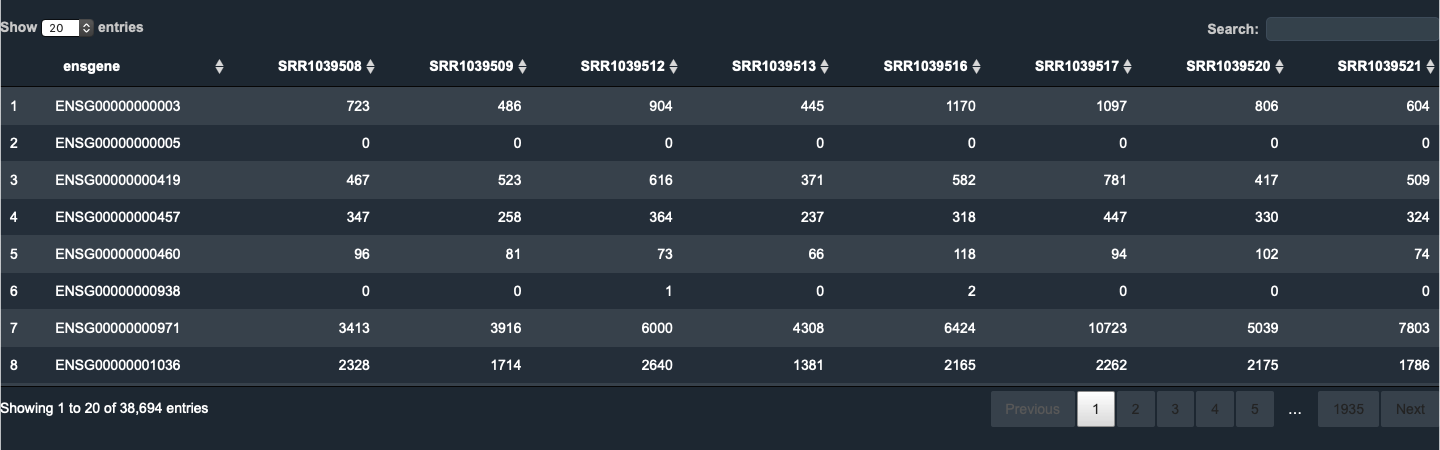
\includegraphics[width=\textwidth]{exTable.png} \sffamily\small\{Figure
? : Exemple de l'importation de la table de comptage. L'utilisateur peut
parcourir les pages de 20 entités du tableaux par une recherche ou en
choisissant la page.\}

\normalsize
\setstretch{1.5}
\setromanfont{Times New Roman}

\hypertarget{partie-3-deseq2}{%
\subsubsection{\texorpdfstring{\normalsize\{Partie 3 :
DESeq2\}}{\{Partie 3 : DESeq2\}}}\label{partie-3-deseq2}}

~~~~~~~ DESeq2 est lancé grâce à un bouton ``Run DESeq2 workflow''. En
appuyant sur sur ce bouton, un écran d'attente va s'afficher le temps
que le processus se termine. Durant cette attente, la fonction
DESeqDataSetFromMatrix() va permettre de stocker les valeurs d'entrée,
les calculs intermédiaires et les résultats d'une analyse de
l'expression différentielle. Afin de faire fonctionner correctement
cette partie, un design est demandé lors de l'importation du fichier
metadata. Ce design doit correspondre à un facteur permettant de
distinguer les deux groupes différents d'échantillons. Il faut donc
faire le bon choix lors de l'élaboration du design garder la ou les
bonnes colonnes du fichier metadata. On appelle une ``colonne linéaire''
une colonne dont toutes les valeurs en lignes sont différentes. Si une
colonnes dite ``linéaire'' se trouve dans le design, alors l'application
risque de crash au moment du lancement du processus DESeq2. Il sera donc
nécessaire de la redémarer. Avec un bon design, le DESeq2 est lancé et
les résultats s'affichent après une dizaine de secondes d'attente.

\par

Ensuite, la fonction DESeq() permet de faire une analyse en 3 étapes :

\begin{itemize}
\item Estimation des facteurs de taille
\item Estimation de la dispersion
\item Ajustement de la loi binomiale négative et test de Wald
\end{itemize}

La statistique de Wald est un test de significativité du coefficient de
régression ; elle est basée sur la propriété de normalité asymptotique
de l'estimation du maximum de vraisemblance. Pour finir le processus
DESeq2, les résultats sont extraits sous forme de tableau grâce à la
fonction results(). Dans ce tableau on retrouve les moyennes des
échantillons, les log2foldchange, les erreurs standards, les
statistiques de tests, les p-values et les p-values ajustées. Ces
résultats vont être importants pour permettre d'établir les graphiques
de la section ``Résultats''.

\hypertarget{partie-4-ruxe9sultats}{%
\subsubsection{\texorpdfstring{\normalsize\{Partie 4 :
Résultats\}}{\{Partie 4 : Résultats\}}}\label{partie-4-ruxe9sultats}}

~~~~~~~ On retrouve plusieurs sortes de résultats sous forme de
graphiques. Tous les graphiques sont faits grâce au package ggplot2 mais
aussi DESeq2 pour le graphique de dispersion et l'ACP et NMF pour les
heatmaps. Tous ces graphiques sont directement disponible dès la fin du
processus de DESeq2 sauf 3. En effet, l'ACP et les deux heatmaps sont
affichés après une seconde étape qui va permettre de lancer les
fonctions capables de réaliser ces graphiques.

\par

Le premier disponible est un graphique de comptage de données (``count
distribution'') qui montre la fréquence de reads par échantillons. Il
est possible de choisir l'échantillon que nous voulons visualiser ainsi
que la porté de l'axe de abscisses et la dimension des barres sur le
graphique. Ensuite, on retrouve un graphique permettant de visualiser le
nombre de reads par échantillons et par gènes. Il y a donc la
possibilité de choisir le gène que l'on veut visualiser. Pour continuer,
nous trouvons un barplot témoignant de la profondeur pour chaque
échantillon avec la possibilité de choisir la largeur des barres. Chacun
de ces trois graphiques proposent une option pour visualiser les données
avant et après normalisation.

\singlespacing

\begin{center}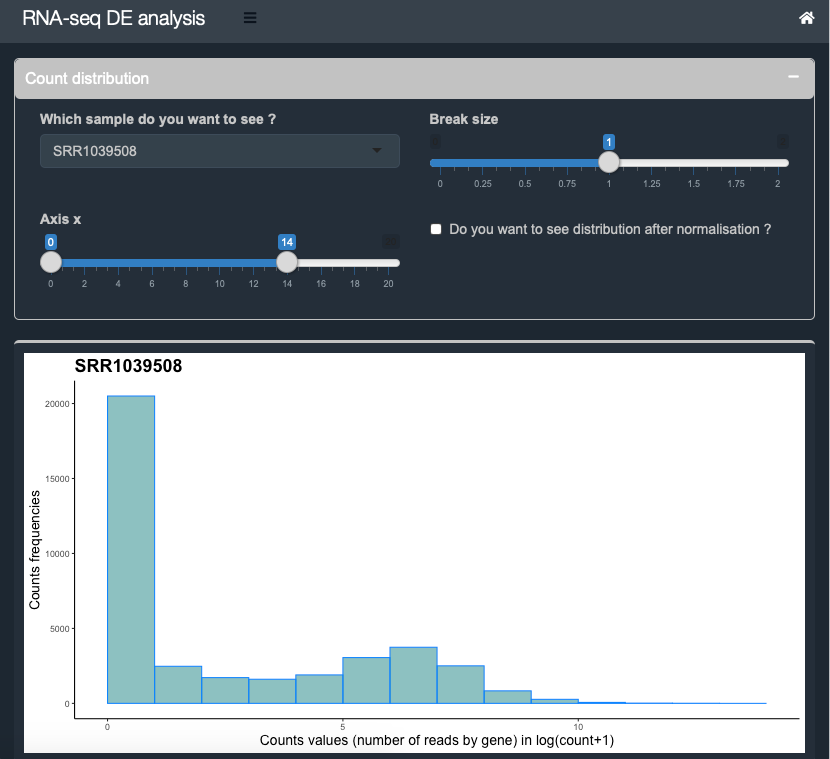
\includegraphics[width=1\linewidth,height=0.3\textheight]{countdistImage} 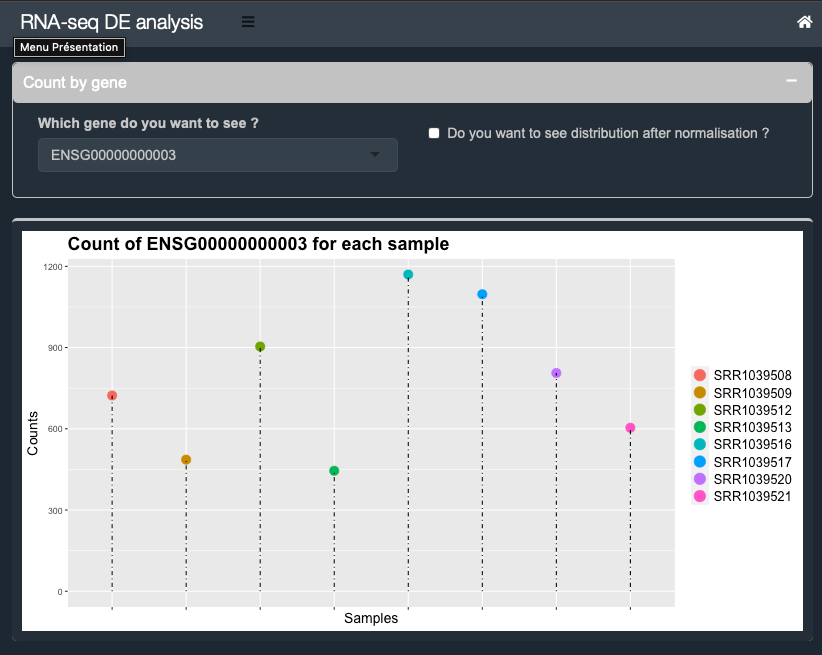
\includegraphics[width=1\linewidth,height=0.3\textheight]{countGene} \end{center}

\sffamily\small\{Figure ? : Exemple de pages pour les graphiques de
count distribution (gauche) et du comptage de reads par gènes (droite).
On remarques les options comme la normalisation, la taille des barres ou
le choix de l'échantillon ou du gène.\}

\setstretch{1.5}
\normalsize
\setromanfont{Times New Roman}

La dispersion est un paramètre décrivant la déviation de la variance par
rapport à la moyenne. Un graphique montrant la relation entre la
dispersion et la moyenne des comptages

\begin{itemize}
\item
  dipsersion
\item
  PCA
\item
  MAplot
\item
  Volcano
\item
  Distance matrix
\item
  Gene expression heatmap
\end{itemize}

Chacun des graphiques est téléchargeable au format .png en bas de chaque
page.

\hypertarget{customisation}{%
\subsubsection{\texorpdfstring{\normalsize\{Customisation\}}{\{Customisation\}}}\label{customisation}}

~~~~~~~ Nous avons utilisé différents outils pour rendre plus agréable
l'utilisation de l'application sur le plan visuel. A l'aide du langage
HTML nous avons pu modifier des thèmes déjà existants. En effet, nous
avons décidé de créer un bouton permettant de choisir entre 2 thèmes :
un thème foncé et un thème clair selon les préférences de l'utilisateur.
Pour cela nous avons utilisé le package \emph{dashboardthemes} qui
propose différents thèmes dont ceux utilisés : grey\_dark et
grey\_light. Il a fallu modifier le thème grey\_dark car il affichait
une police noire sur un fond foncé dans les tableaux. C'était donc
difficilement lisible. Pour se faire, nous avons du récupérer le code du
thème sur le
\href{https://github.com/nik01010/dashboardthemes}{\underline{git}} de
Nik. L. présentant le package et modifier ou ajouter certains codes HTML
directement sur R de façon à ce que tout soit optimisé.

\par

~~~~~~~ Nous avons aussi fait en sorte d'améliorer le visuel de nos
graphiques. Pour cela nous avons donc utilisé ggplot2, le package
permettant de faire des graphiques plus élégants. Ainsi les couleurs,
les tailes des titres et des légendes et le texte sur les graphiques on
pu être modifiés ou ajoutés pour compléter et améliorer au mieux chacun
des graphiques.

\par

~~~~~~~ Pour finir, nous avons mis en place un bouton accueil grâce au
langage HTML. Ce bouton est placé en haut à droite de l'écran, dans
l'en-tête et permet à tout moment de retourner sur la page d'accueil qui
est la page d'information sur l'application. De plus, toujours grâce au
langage HTML, nous avons ajouté un pied de page dans lequel on retrouve
des information sur les développeurs de l'application ainsi que le git
sur lequel on retrouve tout le travail réalisé.

\newpage

\hypertarget{conclusion-et-perspectives}{%
\section{\texorpdfstring{\Large\{Conclusion et
perspectives\}}{\{Conclusion et perspectives\}}}\label{conclusion-et-perspectives}}

Tout d'abord avant de conclure il est important de replacé le projet
dans son contexte. Le but principal était d'aborder de nouveaux outils
nous permettant d'evoluer et progresser sous l'environnement R ainsi que
trouver des outils permettant l'accessibilité à ces mêmes outils. Dans
ce sens ce projet nous a permis de découvrir le depot de package
bioconductor qui fournis de nombreux package destinés à la
bioinformatique et nous avons pu nous concentrer sur l'un de ces
packages DESeq2. Nous avons grâce a ce package appris dans un premier
temps à mieux comprendre l'analyse d'expression differentielle de
données RNA-seq pour ensuite réalisé avec ce package notre propre
analyse d'expression différentielle. Et c'est à partir de cette analyse
que nous avons pu repondre à notre problématique de l'accessibilité, et
nous avons donc réaliser une application simple suivant le workflow de
notre analyse d'expression différentielle sour DESeq2, cette application
permet à tous possesseur d'une table de comptage et de son design
associé de réaliser un workflow de manière automatisé tous en ayant la
possibilité de choisir ses propres paramètres. Toutes la partie création
de cette application nous a permis de découvrir le package shiny et
d'apprendre son utilisation, au dela du package en lui même cette
démarche a permis l'apprentissage de base importante dans le language
html ainsi que quelque point dans le language CSS. La finalité de ce
projet est donc l'acquisition de nouvelles compétences dans l'analyse de
données RNA-seq sous R ainsi que de nouvelles compétences dans
différentes formes de mise en forme de résultats et leurs accessibilités
à d'autres. Maintenant que nous nous sommes familiarisés à ces
différents outils nous pourrions allé plus loin dans notre application
et dans l'analyse de données RNA-seq en étudiant les autres outils
permettant de completer notre analyse nottament en apprenant à utiliser
les packages permettant de réaliser les etapes précedent l'optention de
la table de comptage, ce qui permettra d'avoir une application prête à
l'utilisation dés l'optention des fichier fastQ.

\newpage

\hypertarget{bibliographie}{%
\section{\texorpdfstring{\Large\{Bibliographie\}}{\{Bibliographie\}}}\label{bibliographie}}

\begin{enumerate}
\item Himes BE, Jiang X, Wagner P, et al. RNA-Seq transcriptome profiling identifies CRISPLD2 as a glucocorticoid responsive gene that modulates cytokine function in airway smooth muscle cells. PLoS One. 2014;9(6):e99625. Published 2014 Jun 13. doi: \href{https://journals.plos.org/plosone/article?id=10.1371/journal.pone.0099625}{\underline{10.1371/journal.pone.0099625}}

\item Koch CM, Chiu SF, Akbarpour M, et al. A Beginner's Guide to Analysis of RNA Sequencing Data. Am J Respir Cell Mol Biol. 2018;59(2):145-157. doi: \href{https://www.atsjournals.org/doi/10.1165/rcmb.2017-0430TR}{\underline{10.1165/rcmb.2017-0430TR}}

\item Julien Delafontaine. (2013, septembre 11). Analyse de données RNA-seq : mode d’emploi. Consulté à l’adresse \href{https://bioinfo-fr.net/lanalyse-de-donnees-rna-seq-mode-demploi}{\underline{https://bioinfo-fr.net/lanalyse-de-donnees-rna-seq-mode-demploi}}

\item Bioconductor - Home. (2003). Consulté à l’adresse \href{https://www.bioconductor.org/}{\underline{https://www.bioconductor.org/}}


\item Wickham, H. (2016). Mastering Shiny. Consulté à l’adresse \href{https://mastering-shiny.org/}{\underline{https://mastering-shiny.org/}} 

\item Nik. L. (2018, mars 4). nik01010/dashboardthemes. Consulté à l’adresse
\par
\href{https://github.com/nik01010/dashboardthemes}{\underline{https://github.com/nik01010/dashboardthemes}}
\end{enumerate}
\newpage

\hypertarget{ruxe9sumuxe9}{%
\section{\texorpdfstring{\Large\{Résumé\}}{\{Résumé\}}}\label{ruxe9sumuxe9}}

\hypertarget{abstract}{%
\section{\texorpdfstring{\Large\{Abstract\}}{\{Abstract\}}}\label{abstract}}

\newpage

\hypertarget{annexe-1-script-r-pour-lanalyse-rnaseq-via-deseq2}{%
\section{\texorpdfstring{\Large\{Annexe 1 : Script R pour l'analyse
RNAseq via
DESeq2\}}{\{Annexe 1 : Script R pour l'analyse RNAseq via DESeq2\}}}\label{annexe-1-script-r-pour-lanalyse-rnaseq-via-deseq2}}

\renewcommand{\baselinestretch}{.85}
\scriptsize

\begin{Shaded}
\begin{Highlighting}[]
\CommentTok{#Library}
\KeywordTok{library}\NormalTok{(DESeq2)}
\KeywordTok{library}\NormalTok{(Biobase)}
\KeywordTok{library}\NormalTok{(tidyverse)}

\CommentTok{### import data ----}
\CommentTok{#Firstly we import the 3 data table which we will use during this analysis. }
\CommentTok{#The "counts_table" contains the counting of read mapped on each genes by samples,}
\CommentTok{#"airway_metadata" contains the information about the samples design }
\CommentTok{#and "anno" contains the informations about the genes. }
\NormalTok{counts_table <-}\StringTok{ }\KeywordTok{read.csv}\NormalTok{(}\StringTok{"Data/airway_scaledcounts.csv"}\NormalTok{) }
\NormalTok{airway_metadata <-}\StringTok{ }\KeywordTok{read.csv}\NormalTok{(}\StringTok{"Data/airway_metadata.csv"}\NormalTok{)}
\NormalTok{anno <-}\StringTok{ }\KeywordTok{read.csv}\NormalTok{(}\StringTok{"Data/annotables_grch38.csv"}\NormalTok{)}
\NormalTok{anno <-}\StringTok{ }\NormalTok{anno }\OperatorTok\StringTok{ }\KeywordTok{select}\NormalTok{(ensgene,symbol)}

\CommentTok{### Create the dds object ---}
\NormalTok{dds <-}\StringTok{ }\KeywordTok{DESeqDataSetFromMatrix}\NormalTok{(counts_table,}\DataTypeTok{colData=}\NormalTok{airway_metadata,}\DataTypeTok{design =} \OperatorTok{~}\NormalTok{dex,}\DataTypeTok{tidy =} \OtherTok{TRUE}\NormalTok{)}
\CommentTok{# Set reference of experience, here "control"}
\KeywordTok{colData}\NormalTok{(dds)}\OperatorTok{$}\NormalTok{dex <-}\StringTok{ }\KeywordTok{relevel}\NormalTok{(}\KeywordTok{colData}\NormalTok{(dds)}\OperatorTok{$}\NormalTok{dex , }\DataTypeTok{ref=}\StringTok{"control"}\NormalTok{)}
\CommentTok{# To display experiment design.}
\KeywordTok{colData}\NormalTok{(dds)}
\CommentTok{# To display column which biological condition is set.}
\KeywordTok{design}\NormalTok{(dds)}

\CommentTok{### Explorate data ----}
\CommentTok{#Transformation of dds counts table in data frame to use ggplot package}
\NormalTok{count_table_dds <-}\StringTok{ }\KeywordTok{as.data.frame}\NormalTok{(}\KeywordTok{counts}\NormalTok{(dds))}
\CommentTok{#vizualisation  of count distribution ----}
\CommentTok{#To facilitate the vizualisation we use the log-freq of each count value "log(count+1)"}
\ControlFlowTok{for}\NormalTok{( i }\ControlFlowTok{in} \DecValTok{1}\OperatorTok{:}\DecValTok{8}\NormalTok{)\{}
\NormalTok{  p <-}\StringTok{ }\KeywordTok{ggplot}\NormalTok{(}\DataTypeTok{data=}\NormalTok{count_table_dds, }\KeywordTok{aes}\NormalTok{(}\KeywordTok{log}\NormalTok{(count_dds[,i]}\OperatorTok{+}\DecValTok{1}\NormalTok{))) }\OperatorTok{+}\StringTok{ }
\StringTok{    }\KeywordTok{geom_histogram}\NormalTok{(}\DataTypeTok{breaks=}\KeywordTok{seq}\NormalTok{(}\DecValTok{0}\NormalTok{,}\DecValTok{14}\NormalTok{,}\DecValTok{1}\NormalTok{),}\DataTypeTok{col=}\StringTok{"black"}\NormalTok{,}\DataTypeTok{fill=}\StringTok{"grey"}\NormalTok{)}\OperatorTok{+}
\StringTok{    }\KeywordTok{theme_light}\NormalTok{()}\OperatorTok{+}
\StringTok{    }\KeywordTok{labs}\NormalTok{(}\DataTypeTok{title=}\KeywordTok{colnames}\NormalTok{(count_table_dds)[i], }
         \DataTypeTok{x=}\StringTok{"Count value (number of read by genes) in log(count+1)"}\NormalTok{,}
         \DataTypeTok{y=}\StringTok{"Count frequency"}\NormalTok{) }\OperatorTok{+}\StringTok{ }
\StringTok{    }\KeywordTok{theme_bw}\NormalTok{()}
 \KeywordTok{plot}\NormalTok{(p)}
\NormalTok{\}}
\CommentTok{#Number for Null for each sample ----}
\KeywordTok{apply}\NormalTok{(count_table_dds, }\DecValTok{2}\NormalTok{ ,}\DataTypeTok{FUN =} \ControlFlowTok{function}\NormalTok{(x) }\KeywordTok{sum}\NormalTok{(x}\OperatorTok{==}\DecValTok{0}\NormalTok{))}
\CommentTok{#vizualisation  of depth for each sample using deph.plot function ----}
\NormalTok{depth <-}\StringTok{ }\KeywordTok{colSums}\NormalTok{(count_table_dds) }
\NormalTok{depth <-}\StringTok{ }\KeywordTok{as.data.frame}\NormalTok{(depth)}
\NormalTok{depth}\OperatorTok{$}\NormalTok{sample <-}\StringTok{ }\KeywordTok{row.names}\NormalTok{(depth)}
\KeywordTok{ggplot}\NormalTok{(depth, }\KeywordTok{aes}\NormalTok{( }\DataTypeTok{x=}\NormalTok{sample ,}\DataTypeTok{y=}\NormalTok{depth))}\OperatorTok{+}\StringTok{ }
\StringTok{  }\KeywordTok{geom_bar}\NormalTok{(}\DataTypeTok{stat=}\StringTok{"identity"}\NormalTok{,}\DataTypeTok{col=}\StringTok{"black"}\NormalTok{, }\DataTypeTok{fill=}\StringTok{"white"}\NormalTok{)}\OperatorTok{+}
\StringTok{  }\KeywordTok{labs}\NormalTok{(}\DataTypeTok{title =} \StringTok{"Depth of each sample"}\NormalTok{, }\DataTypeTok{x=}\StringTok{"Sample"}\NormalTok{, }\DataTypeTok{y=}\StringTok{"Depth"}\NormalTok{)}\OperatorTok{+}
\StringTok{  }\KeywordTok{theme_bw}\NormalTok{()}

\CommentTok{#Differential expression analysis and normalization ----}
\NormalTok{dds <-}\StringTok{ }\KeywordTok{DESeq}\NormalTok{(dds)}
\CommentTok{#Extraction of the DE result}
\NormalTok{res <-}\StringTok{ }\KeywordTok{results}\NormalTok{(dds,}\DataTypeTok{tidy =} \OtherTok{TRUE}\NormalTok{)}
\CommentTok{# The scale factor resulting of normalization are stock in size factor of our design.}
\KeywordTok{colData}\NormalTok{(dds) }
\CommentTok{#Depth of count table after normalization ----}
\NormalTok{depth_normalize <-}\StringTok{ }\KeywordTok{colSums}\NormalTok{(}\KeywordTok{counts}\NormalTok{(dds, }\DataTypeTok{normalized=} \OtherTok{TRUE}\NormalTok{))}
\NormalTok{depth_normalize <-}\StringTok{ }\KeywordTok{as.data.frame}\NormalTok{(depth_normalize)}
\NormalTok{depth_normalize}\OperatorTok{$}\NormalTok{sample <-}\StringTok{ }\KeywordTok{row.names}\NormalTok{(depth_normalize)}
\KeywordTok{ggplot}\NormalTok{(depth_normalize, }\KeywordTok{aes}\NormalTok{( }\DataTypeTok{x=}\NormalTok{sample ,}\DataTypeTok{y=}\NormalTok{depth_normalize))}\OperatorTok{+}\StringTok{ }
\StringTok{  }\KeywordTok{geom_bar}\NormalTok{(}\DataTypeTok{stat=}\StringTok{"identity"}\NormalTok{,}\DataTypeTok{col=}\StringTok{"black"}\NormalTok{, }\DataTypeTok{fill=}\StringTok{"white"}\NormalTok{)}\OperatorTok{+}
\StringTok{  }\KeywordTok{labs}\NormalTok{(}\DataTypeTok{title =} \StringTok{"Depth of each sample"}\NormalTok{, }\DataTypeTok{x=}\StringTok{"Sample"}\NormalTok{, }\DataTypeTok{y=}\StringTok{"Depth"}\NormalTok{)}\OperatorTok{+}
\StringTok{  }\KeywordTok{theme_minimal}\NormalTok{()}
\CommentTok{#vizualisation  of count distribution after normalization ----}
\NormalTok{count_normalize <-}\StringTok{ }\KeywordTok{counts}\NormalTok{(dds, }\DataTypeTok{normalized=} \OtherTok{TRUE}\NormalTok{)}
\NormalTok{count_normalize <-}\KeywordTok{as.data.frame}\NormalTok{(count_normalize)}
\ControlFlowTok{for}\NormalTok{(i }\ControlFlowTok{in} \DecValTok{1}\OperatorTok{:}\DecValTok{8}\NormalTok{)\{}
\NormalTok{  p <-}\StringTok{ }\KeywordTok{ggplot}\NormalTok{(}\DataTypeTok{data=}\NormalTok{count_normalize, }\KeywordTok{aes}\NormalTok{(}\KeywordTok{log}\NormalTok{(count_normalize[,i]}\OperatorTok{+}\DecValTok{1}\NormalTok{))) }\OperatorTok{+}\StringTok{ }
\StringTok{    }\KeywordTok{geom_histogram}\NormalTok{(}\DataTypeTok{breaks=}\KeywordTok{seq}\NormalTok{(}\DecValTok{0}\NormalTok{,}\DecValTok{14}\NormalTok{,}\DecValTok{1}\NormalTok{),}\DataTypeTok{col=}\StringTok{"black"}\NormalTok{,}\DataTypeTok{fill=}\StringTok{"grey"}\NormalTok{)}\OperatorTok{+}
\StringTok{    }\KeywordTok{theme_light}\NormalTok{()}\OperatorTok{+}
\StringTok{    }\KeywordTok{labs}\NormalTok{(}\DataTypeTok{title=}\KeywordTok{colnames}\NormalTok{(count_normalize)[i], }
         \DataTypeTok{x=}\StringTok{"Count value (number of read by genes) in log(count+1)"}\NormalTok{,}
         \DataTypeTok{y=}\StringTok{"Count frequency"}\NormalTok{)}
  \KeywordTok{plot}\NormalTok{(p)}
\NormalTok{\}}


\CommentTok{# Dispersion plot ----}
\CommentTok{# Relationship between dispersion and counts means.}
\CommentTok{# DESeq2 offer a function that can directly display a plot which describe }
\CommentTok{#the relation ship beetween dispersion and count mean.}

\NormalTok{DESeq2}\OperatorTok{::}\KeywordTok{plotDispEsts}\NormalTok{(dds, }\DataTypeTok{main=} \StringTok{"Relationship between dispersion and counts means"}\NormalTok{)}
\CommentTok{# We obtain a plot that show the final estimate which are obtain after }
\CommentTok{#shrunk of genes estimate and we finaly observe the fitted estimate. We can also observed outliers value.}

\CommentTok{### DE analysis results ----}

\CommentTok{#Show a summary of DE results at alpha = 0.05}

\KeywordTok{summary}\NormalTok{(}\KeywordTok{results}\NormalTok{(dds),}\FloatTok{0.05}\NormalTok{)}

\CommentTok{# Number of genes wich is differential express at 5%}
\NormalTok{up_regulated <-}\StringTok{ }\NormalTok{res }\OperatorTok\StringTok{ }\KeywordTok{filter}\NormalTok{(padj }\OperatorTok{<=}\StringTok{ }\FloatTok{0.05} \OperatorTok{&}\StringTok{ }\NormalTok{log2FoldChange }\OperatorTok{>}\StringTok{ }\DecValTok{0}\NormalTok{) }\OperatorTok\StringTok{ }\KeywordTok{nrow}\NormalTok{()}
\NormalTok{down_regulated <-}\StringTok{ }\NormalTok{res }\OperatorTok\StringTok{ }\KeywordTok{filter}\NormalTok{(padj }\OperatorTok{<=}\StringTok{ }\FloatTok{0.05} \OperatorTok{&}\StringTok{ }\NormalTok{log2FoldChange }\OperatorTok{<}\StringTok{ }\DecValTok{0}\NormalTok{) }\OperatorTok\StringTok{ }\KeywordTok{nrow}\NormalTok{()}
\NormalTok{tb <-}\StringTok{ }\KeywordTok{table}\NormalTok{(res}\OperatorTok{$}\NormalTok{padj }\OperatorTok{<=}\StringTok{ }\FloatTok{0.05}\NormalTok{, }\DataTypeTok{useNA=}\StringTok{"always"}\NormalTok{)}
\NormalTok{tb.DE <-}\StringTok{ }\KeywordTok{data.frame}\NormalTok{(}\StringTok{"No DE"}\NormalTok{ =}\StringTok{ }\NormalTok{tb[}\DecValTok{1}\NormalTok{], }\StringTok{"Down regulated"}\NormalTok{ =}\StringTok{ }\NormalTok{down_regulated, }
                    \StringTok{"Up regulated"}\NormalTok{ =}\StringTok{ }\NormalTok{up_regulated, }\StringTok{"NA"}\NormalTok{ =}\StringTok{ }\NormalTok{tb[}\DecValTok{3}\NormalTok{]  )}
\KeywordTok{row.names}\NormalTok{(tb.DE) <-}\StringTok{ ""}
\NormalTok{tb.DE}

\CommentTok{# MA plot : relationship between mean count of a gene and it log2 ratio between the two conditions}
\NormalTok{res <-}\StringTok{ }\KeywordTok{as.data.frame}\NormalTok{(res)}
\NormalTok{res <-}\StringTok{ }\NormalTok{res }\OperatorTok\StringTok{ }\KeywordTok{mutate}\NormalTok{(}\DataTypeTok{sig=}\NormalTok{padj}\OperatorTok{<}\FloatTok{0.05}\NormalTok{)}

\KeywordTok{ggplot}\NormalTok{(res, }\KeywordTok{aes}\NormalTok{(}\DataTypeTok{x =}\NormalTok{ baseMean, }\DataTypeTok{y =}\NormalTok{ log2FoldChange, }\DataTypeTok{col =}\NormalTok{ sig)) }\OperatorTok{+}\StringTok{ }
\StringTok{  }\KeywordTok{geom_point}\NormalTok{() }\OperatorTok{+}\StringTok{ }
\StringTok{  }\KeywordTok{scale_x_log10}\NormalTok{() }\OperatorTok{+}
\StringTok{  }\KeywordTok{geom_hline}\NormalTok{(}\DataTypeTok{yintercept =} \DecValTok{0}\NormalTok{, }\DataTypeTok{linetype =} \StringTok{"dashed"}\NormalTok{,}\DataTypeTok{color =} \StringTok{"black"}\NormalTok{) }\OperatorTok{+}\StringTok{ }
\StringTok{  }\KeywordTok{ggtitle}\NormalTok{(}\StringTok{"MA plot"}\NormalTok{) }\OperatorTok{+}\StringTok{ }\KeywordTok{theme_bw}\NormalTok{()}

\CommentTok{#Volcano plot at alpha 0.5}
\CommentTok{#Show ID of the most DE gene }
\NormalTok{res_v <-}\StringTok{ }\NormalTok{res }\OperatorTok\StringTok{ }\KeywordTok{mutate}\NormalTok{(}\DataTypeTok{sig=}\NormalTok{padj}\OperatorTok{<}\FloatTok{0.05}\NormalTok{) }\OperatorTok\StringTok{  }\KeywordTok{arrange}\NormalTok{(padj) }\OperatorTok
\StringTok{  }\KeywordTok{inner_join}\NormalTok{(anno,}\DataTypeTok{by=}\KeywordTok{c}\NormalTok{(}\StringTok{"row"}\NormalTok{=}\StringTok{ "ensgene"}\NormalTok{))}


\KeywordTok{ggplot}\NormalTok{(res_v, }\KeywordTok{aes}\NormalTok{(}\DataTypeTok{x=}\NormalTok{log2FoldChange, }\DataTypeTok{y=}\OperatorTok{-}\KeywordTok{log10}\NormalTok{(padj), }\DataTypeTok{col=}\NormalTok{sig)) }\OperatorTok{+}
\StringTok{  }\KeywordTok{geom_point}\NormalTok{() }\OperatorTok{+}
\StringTok{  }\KeywordTok{ggtitle}\NormalTok{(}\StringTok{"Volcano plot labelling top significant genes"}\NormalTok{) }\OperatorTok{+}
\StringTok{  }\KeywordTok{geom_text_repel}\NormalTok{(}\DataTypeTok{data =} \KeywordTok{subset}\NormalTok{(res_v, (}\OperatorTok{-}\KeywordTok{log10}\NormalTok{(padj) }\OperatorTok{>}\StringTok{ }\DecValTok{30} \OperatorTok{|}\StringTok{ }
\StringTok{                                          }\NormalTok{log2FoldChange }\OperatorTok{>}\StringTok{ }\DecValTok{6} \OperatorTok{|}\StringTok{ }
\StringTok{                                          }\NormalTok{log2FoldChange }\OperatorTok{<}\StringTok{ }\DecValTok{-6}\NormalTok{)),}
                  \KeywordTok{aes}\NormalTok{(}\DataTypeTok{label =}\NormalTok{ symbol),}
                  \DataTypeTok{size =} \DecValTok{4}\NormalTok{,}
                  \DataTypeTok{box.padding =} \KeywordTok{unit}\NormalTok{(}\FloatTok{0.35}\NormalTok{, }\StringTok{"lines"}\NormalTok{),}
                  \DataTypeTok{point.padding =} \KeywordTok{unit}\NormalTok{(}\FloatTok{0.3}\NormalTok{, }\StringTok{"lines"}\NormalTok{), }\DataTypeTok{color =} \StringTok{"darkblue"}\NormalTok{) }\OperatorTok{+}
\StringTok{  }\KeywordTok{scale_colour_discrete}\NormalTok{(}\DataTypeTok{name=}\StringTok{""}\NormalTok{,}
                        \DataTypeTok{labels=}\KeywordTok{c}\NormalTok{(}\StringTok{"Not significative"}\NormalTok{, }\StringTok{"Significative"}\NormalTok{, }\StringTok{"NA"}\NormalTok{)) }\OperatorTok{+}
\StringTok{  }\KeywordTok{guides}\NormalTok{(}\DataTypeTok{color =} \KeywordTok{guide_legend}\NormalTok{(}\DataTypeTok{override.aes =} \KeywordTok{list}\NormalTok{(}\DataTypeTok{size=}\DecValTok{5}\NormalTok{))) }\OperatorTok{+}
\StringTok{  }\KeywordTok{geom_vline}\NormalTok{(}\DataTypeTok{xintercept=}\DecValTok{0}\NormalTok{,}\DataTypeTok{linetype=}\StringTok{"dashed"}\NormalTok{, }\DataTypeTok{color =} \StringTok{"red"}\NormalTok{)}\OperatorTok{+}
\StringTok{  }\KeywordTok{theme}\NormalTok{(}\DataTypeTok{legend.text=}\KeywordTok{element_text}\NormalTok{(}\DataTypeTok{size=}\DecValTok{13}\NormalTok{)) }\OperatorTok{+}
\StringTok{  }\KeywordTok{theme}\NormalTok{(}\DataTypeTok{axis.title.x =} \KeywordTok{element_text}\NormalTok{(}\DataTypeTok{size=}\DecValTok{14}\NormalTok{)) }\OperatorTok{+}
\StringTok{  }\KeywordTok{theme}\NormalTok{(}\DataTypeTok{axis.title.y =} \KeywordTok{element_text}\NormalTok{(}\DataTypeTok{size=}\DecValTok{14}\NormalTok{))}

\CommentTok{# PCA}
\CommentTok{# Two PCA with two different transformation}
\NormalTok{vsdata <-}\StringTok{ }\KeywordTok{vst}\NormalTok{(dds, }\DataTypeTok{blind=}\OtherTok{FALSE}\NormalTok{)}
\KeywordTok{plotPCA}\NormalTok{(vsdata, }\DataTypeTok{intgroup=}\StringTok{"dex"}\NormalTok{)}

\NormalTok{rld <-}\StringTok{ }\KeywordTok{rlogTransformation}\NormalTok{(dds, }\DataTypeTok{blind =} \OtherTok{FALSE}\NormalTok{)}
\KeywordTok{plotPCA}\NormalTok{(rld, }\DataTypeTok{intgroup=}\StringTok{"dex"}\NormalTok{)}

\CommentTok{#Distance matrix for sample}
\KeywordTok{library}\NormalTok{(RColorBrewer)}
\KeywordTok{library}\NormalTok{(gplots)}
\NormalTok{dists <-}\StringTok{ }\KeywordTok{dist}\NormalTok{(}\KeywordTok{t}\NormalTok{(}\KeywordTok{assay}\NormalTok{(vsdata)))}
\NormalTok{mat <-}\StringTok{ }\KeywordTok{as.matrix}\NormalTok{(dists)}
\NormalTok{hmcol=}\KeywordTok{colorRampPalette}\NormalTok{(}\KeywordTok{brewer.pal}\NormalTok{(}\DecValTok{9}\NormalTok{,}\StringTok{"GnBu"}\NormalTok{))(}\DecValTok{100}\NormalTok{)}
\KeywordTok{heatmap.2}\NormalTok{(mat,}\DataTypeTok{trace=}\StringTok{"none"}\NormalTok{,}\DataTypeTok{col =} \KeywordTok{rev}\NormalTok{(hmcol),}\DataTypeTok{margin=}\KeywordTok{c}\NormalTok{(}\DecValTok{13}\NormalTok{,}\DecValTok{13}\NormalTok{))}

\CommentTok{#Heatmap of gene expression for 50 better DE gene}
\KeywordTok{library}\NormalTok{(NMF)}
\NormalTok{res <-}\StringTok{ }\KeywordTok{tbl_df}\NormalTok{(res)}
\NormalTok{res <-}\StringTok{ }\NormalTok{res }\OperatorTok\StringTok{ }
\StringTok{  }\KeywordTok{arrange}\NormalTok{(padj) }\OperatorTok\StringTok{ }
\StringTok{  }\KeywordTok{inner_join}\NormalTok{(anno,}\DataTypeTok{by=}\KeywordTok{c}\NormalTok{(}\StringTok{"row"}\NormalTok{=}\StringTok{"ensgene"}\NormalTok{)) }\OperatorTok
\StringTok{  }\KeywordTok{filter}\NormalTok{(padj}\OperatorTok{<}\FloatTok{0.05}\NormalTok{)}
\NormalTok{NMF}\OperatorTok{::}\KeywordTok{aheatmap}\NormalTok{(}\KeywordTok{assay}\NormalTok{(vsdata)[}\KeywordTok{arrange}\NormalTok{(res, padj, pvalue)}\OperatorTok{$}\NormalTok{row[}\DecValTok{1}\OperatorTok{:}\DecValTok{50}\NormalTok{],], }
              \DataTypeTok{labRow=}\KeywordTok{arrange}\NormalTok{(res, padj, pvalue)}\OperatorTok{$}\NormalTok{symbol[}\DecValTok{1}\OperatorTok{:}\DecValTok{50}\NormalTok{], }
              \DataTypeTok{scale=}\StringTok{"row"}\NormalTok{, }\DataTypeTok{distfun=}\StringTok{"pearson"}\NormalTok{, }
              \DataTypeTok{annCol=}\NormalTok{dplyr}\OperatorTok{::}\KeywordTok{select}\NormalTok{(airway_metadata, dex, celltype), }
              \DataTypeTok{col=}\KeywordTok{c}\NormalTok{(}\StringTok{"green"}\NormalTok{,}\StringTok{"black"}\NormalTok{,}\StringTok{"black"}\NormalTok{,}\StringTok{"red"}\NormalTok{))}
\end{Highlighting}
\end{Shaded}

\normalsize

\newpage

\hypertarget{annexe-2-scripts-r-pour-lapplication-shiny}{%
\section{\texorpdfstring{\Large\{Annexe 2 : Scripts R pour l'application
Shiny\}}{\{Annexe 2 : Scripts R pour l'application Shiny\}}}\label{annexe-2-scripts-r-pour-lapplication-shiny}}

\hypertarget{interface-utilisateur}{%
\subsection{\texorpdfstring{\large\{2.1 Interface
utilisateur\}}{\{2.1 Interface utilisateur\}}}\label{interface-utilisateur}}

\renewcommand{\baselinestretch}{.85}
\scriptsize

\begin{Shaded}
\begin{Highlighting}[]
\CommentTok{### Library ----}
\CommentTok{### here we find all library need for proper functionning of app}
\KeywordTok{library}\NormalTok{(shiny)}
\KeywordTok{library}\NormalTok{(shinydashboard)}
\KeywordTok{library}\NormalTok{(shinyjs)}
\KeywordTok{library}\NormalTok{(dplyr)}
\KeywordTok{library}\NormalTok{(tidyverse)}
\KeywordTok{library}\NormalTok{(vroom)}
\KeywordTok{library}\NormalTok{(DT)}
\KeywordTok{library}\NormalTok{(DESeq2)}
\KeywordTok{library}\NormalTok{(shinyWidgets)}
\KeywordTok{library}\NormalTok{(shinythemes)}
\KeywordTok{library}\NormalTok{(waiter)}
\KeywordTok{library}\NormalTok{(dashboardthemes)}
\KeywordTok{library}\NormalTok{(shinycssloaders)}
\KeywordTok{library}\NormalTok{(shinydashboardPlus)}
\CommentTok{### Files with all the function needed to make plots ----}
\KeywordTok{source}\NormalTok{(}\StringTok{"function_dds.R"}\NormalTok{)}

\CommentTok{### Annotation pannel ----}
\NormalTok{parameters_Annotation <-}\StringTok{ }\KeywordTok{tagList}\NormalTok{(}
\NormalTok{  tags}\OperatorTok{$}\KeywordTok{style}\NormalTok{(}\StringTok{"#paramsAnno \{ display:none; \}"}\NormalTok{),}
\CommentTok{### parameter_tabs is a tabsetPanel for input annotation page}
\CommentTok{### it allow to switch between panel when we use updateTabsetPanel()}
\CommentTok{### in our case it is when we check right annotation boxes of input annotation page}
  \KeywordTok{tabsetPanel}\NormalTok{(}
    \DataTypeTok{id=}\StringTok{"paramsAnno"}\NormalTok{,}
    \KeywordTok{tabPanel}\NormalTok{(}\StringTok{"nothing"}\NormalTok{),  }
    \KeywordTok{tabPanel}\NormalTok{(}\StringTok{"annotation"}\NormalTok{,}
             \KeywordTok{fluidRow}\NormalTok{(}
               \KeywordTok{column}\NormalTok{(}\DataTypeTok{width=} \DecValTok{6}\NormalTok{,}
                      \KeywordTok{box}\NormalTok{(}\DataTypeTok{title=}\StringTok{"Upload annotation file"}\NormalTok{,}\DataTypeTok{width =} \DecValTok{12}\NormalTok{, }\DataTypeTok{solidHeader =} \OtherTok{TRUE}\NormalTok{,}\DataTypeTok{collapsible =} \OtherTok{TRUE}\NormalTok{,}
                          \KeywordTok{column}\NormalTok{(}\DataTypeTok{width=}\DecValTok{5}\NormalTok{,}\KeywordTok{selectInput}\NormalTok{(}\StringTok{"sep_Anno"}\NormalTok{, }\StringTok{"Separator:"}\NormalTok{, }\KeywordTok{c}\NormalTok{(}\StringTok{"Comma"}\NormalTok{ =}\StringTok{ ","}\NormalTok{, }\StringTok{"Tab"}\NormalTok{ =}\StringTok{ "}\CharTok{\textbackslash{}t}\StringTok{"}\NormalTok{, }
                  \StringTok{"Semi-colon"}\NormalTok{ =}\StringTok{ ";"}\NormalTok{))),}
                          \KeywordTok{fileInput}\NormalTok{(}\StringTok{"AnnotationFile"}\NormalTok{, }\StringTok{"Upload annotation file"}\NormalTok{, }
                                    \DataTypeTok{accept =} \KeywordTok{c}\NormalTok{(}\StringTok{".csv"}\NormalTok{,}\StringTok{".txt"}\NormalTok{,}\StringTok{".tsv"}\NormalTok{)))),}
               \KeywordTok{column}\NormalTok{(}\DataTypeTok{width=} \DecValTok{6}\NormalTok{,     }
                      \KeywordTok{box}\NormalTok{(}
                        \DataTypeTok{title =} \StringTok{"Accepted files :"}\NormalTok{, }\DataTypeTok{width =} \DecValTok{12}\NormalTok{,}
                        \KeywordTok{HTML}\NormalTok{(}
                          \StringTok{"<li> .csv / .tsv / .txt files </li>}
\StringTok{                          <li> Separated by tabulation, comma or semi-colon </li>}
\StringTok{                          <li> One column with genes symbols named 'symbol'</li>}
\StringTok{                          "}\NormalTok{),}
                        \DataTypeTok{height =} \DecValTok{160}
\NormalTok{                        )}
\NormalTok{                      )}
\NormalTok{                    )}
\NormalTok{                )}
\NormalTok{            )}
\NormalTok{          )}

\CommentTok{### User Interface  ----}
\CommentTok{### UI is a shinydashboard, we use library shinydashboard to set up a dashboard UI}
\CommentTok{### a dashboard is compound of :}
\CommentTok{###   - a Header}
\CommentTok{###   - a sidebar}
\CommentTok{###   - a body }
\NormalTok{ui <-}\StringTok{ }\KeywordTok{tagList}\NormalTok{(}
  \CommentTok{### Parameters of the dashboard ----}
  \KeywordTok{div}\NormalTok{(}
    \DataTypeTok{id =} \StringTok{"app"}\NormalTok{,}
    \KeywordTok{dashboardPage}\NormalTok{(}
      \CommentTok{### Customize the header ----}
      \CommentTok{### header is composate of :}
      \CommentTok{###   - a title }
      \CommentTok{###   - a home bouton which on click return user on introduction page}
      \KeywordTok{dashboardHeader}\NormalTok{(}\DataTypeTok{title =} \StringTok{"RNA-seq DE analysis"}\NormalTok{, }
                      \KeywordTok{uiOutput}\NormalTok{(}\StringTok{"themes"}\NormalTok{),}
                     
                      \CommentTok{### Home button ----}
\NormalTok{                      tags}\OperatorTok{$}\KeywordTok{li}\NormalTok{(}\KeywordTok{a}\NormalTok{(}\DataTypeTok{onclick =} \StringTok{"openTab('Intro')"}\NormalTok{,}
                                \DataTypeTok{href =} \OtherTok{NULL}\NormalTok{,}
                                \KeywordTok{icon}\NormalTok{(}\StringTok{"home"}\NormalTok{),}
                                \DataTypeTok{title =} \StringTok{"Homepage"}\NormalTok{,}
                                \DataTypeTok{style =} \StringTok{"cursor: pointer;"}\NormalTok{),}
                              \DataTypeTok{class =} \StringTok{"dropdown"}\NormalTok{,}
\NormalTok{                              tags}\OperatorTok{$}\KeywordTok{script}\NormalTok{(}\KeywordTok{HTML}\NormalTok{(}\StringTok{"}
\StringTok{                                               var openTab = function(tabName)\{}
\StringTok{                                               $('a', $('.sidebar')).each(function() \{}
\StringTok{                                               if(this.getAttribute('data-value') == tabName) \{}
\StringTok{                                               this.click()}
\StringTok{                                               \};}
\StringTok{                                               \});}
\StringTok{                                               \}"}\NormalTok{)))}
\NormalTok{      ),}
      
      \CommentTok{### Sidebar ----}
      \CommentTok{### Sider bar  is composate of a sidebar menu}
      \CommentTok{### in this sidebar menu we have menu item which is associate with a tab of body dashboard }
      \KeywordTok{dashboardSidebar}\NormalTok{(}
        \KeywordTok{sidebarMenu}\NormalTok{(}\DataTypeTok{id=}\StringTok{"mysidebar"}\NormalTok{,}
            \KeywordTok{menuItem}\NormalTok{(}\DataTypeTok{text =} \StringTok{"Informations"}\NormalTok{, }\DataTypeTok{tabName =} \StringTok{"Intro"}\NormalTok{, }\DataTypeTok{icon =} \KeywordTok{icon}\NormalTok{(}\StringTok{"info-circle"}\NormalTok{)),}
            \KeywordTok{menuItem}\NormalTok{(}\DataTypeTok{text =} \StringTok{"1 Upload data"}\NormalTok{, }\DataTypeTok{tabName =} \StringTok{"upload"}\NormalTok{, }\DataTypeTok{icon =} \KeywordTok{icon}\NormalTok{(}\StringTok{"arrow-circle-up"}\NormalTok{),}
                     \DataTypeTok{startExpanded =} \OtherTok{TRUE}\NormalTok{,}
                        \CommentTok{# menuItem which are set up in the server function}
                      \KeywordTok{menuItemOutput}\NormalTok{(}\StringTok{"CountTable"}\NormalTok{),}
                      \KeywordTok{menuItemOutput}\NormalTok{(}\StringTok{"MetadataTable"}\NormalTok{),}
                      \KeywordTok{menuItemOutput}\NormalTok{(}\StringTok{"AnnotationTable"}\NormalTok{)),}
            \KeywordTok{menuItem}\NormalTok{(}\DataTypeTok{text =} \StringTok{"2 Run DESeq2"}\NormalTok{, }\DataTypeTok{tabName =} \StringTok{"deseq2"}\NormalTok{, }\DataTypeTok{icon =} \KeywordTok{icon}\NormalTok{(}\StringTok{"play-circle"}\NormalTok{)),}
            \KeywordTok{menuItemOutput}\NormalTok{(}\StringTok{"menuResults"}\NormalTok{),}
\NormalTok{            tags}\OperatorTok{$}\KeywordTok{hr}\NormalTok{(),}\CommentTok{# a simple line }
            \CommentTok{# this menu generate a switch button to set theme of dashboard}
            \CommentTok{# two options are available a light or dark mode}
            \KeywordTok{menuItem}\NormalTok{(}\DataTypeTok{icon =} \OtherTok{NULL}\NormalTok{,}
            \KeywordTok{materialSwitch}\NormalTok{(}\DataTypeTok{inputId =} \StringTok{"theme"}\NormalTok{, }\DataTypeTok{label =} \StringTok{"Theme"}\NormalTok{, }\DataTypeTok{status =} \StringTok{"default"}\NormalTok{, }\DataTypeTok{value=} \OtherTok{TRUE}\NormalTok{)}
\NormalTok{            ),tags}\OperatorTok{$}\KeywordTok{hr}\NormalTok{()}
\NormalTok{        )}
\NormalTok{      ),}
      \CommentTok{### Dashboard body ----}
      \CommentTok{### Organization of the differents pages associate with their menuItem}
      \KeywordTok{dashboardBody}\NormalTok{(}
        \KeywordTok{useShinyjs}\NormalTok{(),}
        \KeywordTok{fluidRow}\NormalTok{(}
          \KeywordTok{tabItems}\NormalTok{(}
            \CommentTok{### Introduction ----}
            \CommentTok{### introduction page associate with menuItem "Informations"}
            \CommentTok{### In this page we find all information about application}
            \CommentTok{### in particular how it works and different tool used to generate DE analysis}
            \CommentTok{### to generate layout html tag provide by shiny library are used }
            \CommentTok{### withSpinner() of shinycssloaders library is use to generate waiting screen during load of img}
            \KeywordTok{tabItem}\NormalTok{(}\DataTypeTok{tabName =} \StringTok{"Intro"}\NormalTok{,}
                    \KeywordTok{fluidPage}\NormalTok{(}
                      \KeywordTok{h2}\NormalTok{(}\StringTok{"Introduction"}\NormalTok{),}
                      \KeywordTok{p}\NormalTok{(}\StringTok{"This is an R Shiny web interactive application developed as part of a "}\NormalTok{, }
                        \KeywordTok{strong}\NormalTok{(}\StringTok{"course project."}\NormalTok{), }\StringTok{"The purpose of this application is to perform a "}\NormalTok{,}
                        \KeywordTok{strong}\NormalTok{(}\StringTok{"differential expression analysis from a counts table"}\NormalTok{), }
                        \StringTok{"in order to help }
\StringTok{                        researchers getting interpretable results."}\NormalTok{,}
                        \DataTypeTok{align =} \StringTok{"justify"}\NormalTok{),}
                      \KeywordTok{p}\NormalTok{(}\StringTok{"This application uses the package "}\NormalTok{, }
                        \KeywordTok{a}\NormalTok{(}\StringTok{"DESeq2"}\NormalTok{, }\DataTypeTok{href=}\StringTok{"https://bioconductor.org/packages/release/bioc/html/DESeq2.html"}\NormalTok{), }
                        \StringTok{"from Bioconductor. It is a package to study differential gene expression analysis }
\StringTok{                        based on the negative binomial distribution. It allows a quick visualization of results }
\StringTok{                        in order to analyze the counts table data. The results will be given in different forms }
\StringTok{                        like graphics, heatmaps, MAplot or even Volcano plot."}\NormalTok{,}
                        \DataTypeTok{align =} \StringTok{"justify"}\NormalTok{),}
\NormalTok{                      tags}\OperatorTok{$}\KeywordTok{hr}\NormalTok{(),}
                      \KeywordTok{h3}\NormalTok{(}\StringTok{"1. Upload data"}\NormalTok{, }\DataTypeTok{style=}\StringTok{"padding-left: 1em"}\NormalTok{),}
                      \KeywordTok{p}\NormalTok{(}\StringTok{"The input data files accepted for this App are 3 files in '.txt', '.csv' or '.tsv' }
\StringTok{                      format separated by comma, tabulation or semi-colon.}
\StringTok{                        This App necessarily requires a 'Count Data Table' and a 'Metadata Table'. An optional }
\StringTok{                      'Annotation File' can be added"}\NormalTok{, }\DataTypeTok{style=}\StringTok{"padding-left: 2em"}\NormalTok{, }\DataTypeTok{align =} \StringTok{"justify"}\NormalTok{),}
                      \KeywordTok{h4}\NormalTok{(}\StringTok{"1.1 Count Data Table"}\NormalTok{, }\DataTypeTok{style=}\StringTok{"padding-left: 3em"}\NormalTok{),}
                      \KeywordTok{p}\NormalTok{(}\StringTok{"The Count Data Table must contain the count for each sample of the experiment for each }
\StringTok{                        gene and the first column must be gene ID or gene name as below :"}\NormalTok{,}
                        \DataTypeTok{style=}\StringTok{"padding-left: 5em"}\NormalTok{, }\DataTypeTok{align =} \StringTok{"justify"}\NormalTok{),}
                      \KeywordTok{column}\NormalTok{( }\DecValTok{12}\NormalTok{, }\DataTypeTok{style=}\StringTok{"padding-left: 5em"}\NormalTok{ ,}\KeywordTok{withSpinner}\NormalTok{(}\KeywordTok{tableOutput}\NormalTok{(}\StringTok{"countExample"}\NormalTok{))),}
                      \KeywordTok{br}\NormalTok{(),}
                      \KeywordTok{h4}\NormalTok{(}\StringTok{"1.2 Metadata Table"}\NormalTok{, }\DataTypeTok{style=}\StringTok{"padding-left: 3em"}\NormalTok{),}
                      \KeywordTok{p}\NormalTok{(}\StringTok{"The Metadata table must contain the information of the experiment with at least }
\StringTok{                      2 columns. The first one corresponds to the samples in the same order as the columns of }
\StringTok{                      the Count Table. }
\StringTok{                        The second one is a condition column. You can add as many columns as you have factors }
\StringTok{                      in your experiment."}\NormalTok{,}\DataTypeTok{style=}\StringTok{"padding-left: 5em"}\NormalTok{, }\DataTypeTok{align =} \StringTok{"justify"}\NormalTok{),}
                      \KeywordTok{column}\NormalTok{( }\DecValTok{12}\NormalTok{, }\DataTypeTok{style=}\StringTok{"padding-left: 5em"}\NormalTok{ ,}\KeywordTok{withSpinner}\NormalTok{(}\KeywordTok{tableOutput}\NormalTok{(}\StringTok{"metadataExample"}\NormalTok{))),}
                      \KeywordTok{h4}\NormalTok{(}\StringTok{"1.2  Annotation File"}\NormalTok{, }\DataTypeTok{style=}\StringTok{"padding-left: 3em"}\NormalTok{),}
                      \KeywordTok{p}\NormalTok{(}\StringTok{"The Annotation File contains informations about the genes. If you have one, it must }
\StringTok{                        contain a column named 'symbol' in which we can find the symbol of each gene."}\NormalTok{,}
                        \DataTypeTok{style=}\StringTok{"padding-left: 5em"}\NormalTok{, }\DataTypeTok{align =} \StringTok{"justify"}\NormalTok{),}
                      \KeywordTok{column}\NormalTok{( }\DecValTok{12}\NormalTok{, }\DataTypeTok{style=}\StringTok{"padding-left: 5em"}\NormalTok{ ,}\KeywordTok{withSpinner}\NormalTok{(}\KeywordTok{tableOutput}\NormalTok{(}\StringTok{"annoExample"}\NormalTok{))),}
                      \KeywordTok{h3}\NormalTok{(}\StringTok{"2. Results"}\NormalTok{, }\DataTypeTok{style=}\StringTok{"padding-left: 1em"}\NormalTok{),}
                      \KeywordTok{p}\NormalTok{(}\StringTok{"The results will be display after running DESeq2. You will obtain 9 differents }
\StringTok{                        results :"}\NormalTok{, }\DataTypeTok{style=}\StringTok{"padding-left: 2em"}\NormalTok{, }\DataTypeTok{align =} \StringTok{"justify"}\NormalTok{),}
                      \KeywordTok{p}\NormalTok{(}\StringTok{"- Count distribution"}\NormalTok{,}
                        \KeywordTok{br}\NormalTok{(), }\StringTok{"- Count by gene"}\NormalTok{,}
                        \KeywordTok{br}\NormalTok{(), }\StringTok{"- Depth of sample"}\NormalTok{,}
                        \KeywordTok{br}\NormalTok{(), }\StringTok{"- Dispersion"}\NormalTok{,}
                        \KeywordTok{br}\NormalTok{(), }\StringTok{"- PCA"}\NormalTok{,}
                        \KeywordTok{br}\NormalTok{(), }\StringTok{"- MA plot"}\NormalTok{,}
                        \KeywordTok{br}\NormalTok{(), }\StringTok{"- Volcano plot"}\NormalTok{,}
                        \KeywordTok{br}\NormalTok{(), }\StringTok{"- Distance matrix"}\NormalTok{,}
                        \KeywordTok{br}\NormalTok{(), }\StringTok{"- Heatmap"}\NormalTok{,}\DataTypeTok{style=}\StringTok{"padding-left: 5em"}\NormalTok{, }\DataTypeTok{align =} \StringTok{"justify"}\NormalTok{),}
                      \KeywordTok{p}\NormalTok{(}\StringTok{"You can download all the results plots at the bottom of all these pages."}\NormalTok{,  }
                        \DataTypeTok{style=}\StringTok{"padding-left: 2em"}\NormalTok{, }\DataTypeTok{align =} \StringTok{"justify"}\NormalTok{)}
\NormalTok{                      )}
\NormalTok{                    ),}
            \CommentTok{### Upload count table ----}
            \CommentTok{### upload page of count table of RNA-seq experience}
            \CommentTok{### this page is associate with menuItemOuput("")}
            \CommentTok{### On this page we find :}
            \CommentTok{###   - a box which countain :}
            \CommentTok{###       - a selectInput of separator }
            \CommentTok{###       - a fileInput to upload count table of RNA-seq experience}
            \CommentTok{###   - a box which countain :}
            \CommentTok{###       - information about file accepted in fileInput }
            \CommentTok{###   - a dataTableOutput of count table input in fileInput}
            \KeywordTok{tabItem}\NormalTok{(}\DataTypeTok{tabName =} \StringTok{"CountData"}\NormalTok{,}
                    \KeywordTok{column}\NormalTok{(}\DataTypeTok{width =} \DecValTok{6}\NormalTok{,}
                           \KeywordTok{box}\NormalTok{(}\DataTypeTok{title=}\StringTok{"Upload count table"}\NormalTok{,}\DataTypeTok{width =} \DecValTok{12}\NormalTok{, }\DataTypeTok{solidHeader =} \OtherTok{TRUE}\NormalTok{,}\DataTypeTok{collapsible =} \OtherTok{TRUE}\NormalTok{,}
                               \KeywordTok{column}\NormalTok{(}\DataTypeTok{width=}\DecValTok{5}\NormalTok{,}
                                      \KeywordTok{selectInput}\NormalTok{(}\StringTok{"separator_Count"}\NormalTok{, }\StringTok{"Separator:"}\NormalTok{, }\KeywordTok{c}\NormalTok{(}\StringTok{"Comma"}\NormalTok{ =}\StringTok{ ","}\NormalTok{,                                                                                     }\StringTok{"Tab"}\NormalTok{ =}\StringTok{ "}\CharTok{\textbackslash{}t}\StringTok{"}\NormalTok{, }\StringTok{"Semi-colon"}\NormalTok{ =}\StringTok{ ";"}\NormalTok{))),}
                               \KeywordTok{fileInput}\NormalTok{(}\StringTok{"CountDataTable"}\NormalTok{, }\StringTok{"Upload count table"}\NormalTok{, }
                                         \DataTypeTok{accept =} \KeywordTok{c}\NormalTok{(}\StringTok{".csv"}\NormalTok{,}\StringTok{".txt"}\NormalTok{,}\StringTok{".tsv"}\NormalTok{))}
\NormalTok{                           )),}
                    \KeywordTok{column}\NormalTok{(}\DataTypeTok{width =} \DecValTok{6}\NormalTok{,}
                           \KeywordTok{box}\NormalTok{(}
                             \DataTypeTok{title =} \StringTok{"Accepted files :"}\NormalTok{, }\DataTypeTok{width =} \DecValTok{12}\NormalTok{,}
                             \KeywordTok{HTML}\NormalTok{(}
                               \StringTok{"<li> .csv / .tsv / .txt files </li>}
\StringTok{                               <li> Separated by tabulation, comma or semi-colon </li>}
\StringTok{                               <li> First column has to be gene ID or gene name</li>}
\StringTok{                               <li> All others columns are count for each sample</li>"}\NormalTok{),}
                             \DataTypeTok{height =} \DecValTok{160}
\NormalTok{                             )),}
                    \KeywordTok{dataTableOutput}\NormalTok{(}\StringTok{"CountReadTable"}\NormalTok{)}
\NormalTok{                    ),}
            \CommentTok{### Upload metadata table ----}
            \CommentTok{### upload page of metadata file of RNA-seq experience}
            \CommentTok{### this page is associate with menuItemOuput("")}
            \CommentTok{### On this page we find :}
            \CommentTok{###   - a box which countain :}
            \CommentTok{###       - a selectInput of separator }
            \CommentTok{###       - a fileInput to upload metadata of RNA-seq experience}
            \CommentTok{###   - a box which countain :}
            \CommentTok{###       - information about file accepted in fileInput}
            \CommentTok{###   - a box which countain :}
            \CommentTok{###       - a text input to chose design formula to set for DESeq2 dataset object}
            \CommentTok{###   - a dataTableOutput of metadata input in fileInput}
                  \KeywordTok{tabItem}\NormalTok{(}\DataTypeTok{tabName =} \StringTok{"Metadata"}\NormalTok{,}
                    \KeywordTok{column}\NormalTok{(}\DataTypeTok{width =} \DecValTok{6}\NormalTok{,}
                           \KeywordTok{box}\NormalTok{(}\DataTypeTok{title=}\StringTok{"Upload metadata table"}\NormalTok{,}\DataTypeTok{width =} \DecValTok{12}\NormalTok{, }\DataTypeTok{solidHeader =} \OtherTok{TRUE}\NormalTok{,}\DataTypeTok{collapsible =} \OtherTok{TRUE}\NormalTok{,}
                               \KeywordTok{column}\NormalTok{(}\DataTypeTok{width=}\DecValTok{5}\NormalTok{,}
                                      \KeywordTok{selectInput}\NormalTok{(}\StringTok{"separator_Metadata"}\NormalTok{, }\StringTok{"Separator:"}\NormalTok{, }
                                                  \KeywordTok{c}\NormalTok{(}\StringTok{"Comma"}\NormalTok{ =}\StringTok{ ","}\NormalTok{, }\StringTok{"Tab"}\NormalTok{ =}\StringTok{ "}\CharTok{\textbackslash{}t}\StringTok{"}\NormalTok{, }\StringTok{"Semi-colon"}\NormalTok{ =}\StringTok{ ";"}\NormalTok{))),}
                               \KeywordTok{fileInput}\NormalTok{(}\StringTok{"MetadataFile"}\NormalTok{, }\StringTok{"Upload metadata table"}\NormalTok{, }
                                         \DataTypeTok{accept =} \KeywordTok{c}\NormalTok{(}\StringTok{".csv"}\NormalTok{,}\StringTok{".txt"}\NormalTok{,}\StringTok{".tsv"}\NormalTok{))}
\NormalTok{                           )),}
                    \KeywordTok{column}\NormalTok{(}\DataTypeTok{width =} \DecValTok{6}\NormalTok{,}
                           \KeywordTok{box}\NormalTok{(}
                             \DataTypeTok{title =} \StringTok{"Accepted files :"}\NormalTok{, }\DataTypeTok{width =} \DecValTok{12}\NormalTok{,}
                             \KeywordTok{HTML}\NormalTok{(}
                               \StringTok{"<li> .csv / .tsv / .txt files </li>}
\StringTok{                               <li> Separated by tabulation, comma or semi-colon </li>}
\StringTok{                               <li> At least metadata table contains two columns</li>}
\StringTok{                               <li> At least one column has to be factor</li>"}\NormalTok{),}
                             \DataTypeTok{height =} \DecValTok{160}
\NormalTok{                             )),}
                    \KeywordTok{column}\NormalTok{(}\DataTypeTok{width =} \DecValTok{12}\NormalTok{,}
                           \KeywordTok{box}\NormalTok{(}\DataTypeTok{width =} \DecValTok{12}\NormalTok{,}
                               \KeywordTok{textInput}\NormalTok{(}\StringTok{"DesignDESeq2"}\NormalTok{,}\StringTok{"Choose your design without linear combination"}\NormalTok{, }
                                         \DataTypeTok{placeholder =} \StringTok{"Conditions"}\NormalTok{))),}
                    \KeywordTok{dataTableOutput}\NormalTok{(}\StringTok{"MetaTable"}\NormalTok{)}
\NormalTok{                    ),}
            \CommentTok{### Upload annotation file ----}
            \CommentTok{### upload page of annotation file associate with the RNA-seq experience}
            \CommentTok{### this page is associate with menuItemOuput("")}
            \CommentTok{### on this page we find :}
            \CommentTok{###   - a box with :}
            \CommentTok{###       - a checkboxInput :  }
            \CommentTok{###            - if box is check on : parameter_tabs is set on annotation}
            \CommentTok{###               - On this page we find :}
            \CommentTok{###                   - a box which countain :}
            \CommentTok{###                       - a selectInput of separator }
            \CommentTok{###                       - a fileInput to upload metadata of RNA-seq experience}
            \CommentTok{###                   - a box which countain :}
            \CommentTok{###                       - information about file accepted in fileInput}
            \CommentTok{###            - if box is check off : parameter_tabs is set on nothing}
            \CommentTok{###               - On this page we find : nothing }
              \KeywordTok{tabItem}\NormalTok{(}\DataTypeTok{tabName =} \StringTok{"Annotation"}\NormalTok{,}
                    \KeywordTok{fluidPage}\NormalTok{(}
                      \KeywordTok{box}\NormalTok{(}\DataTypeTok{width =} \DecValTok{12}\NormalTok{,}
                          \KeywordTok{checkboxInput}\NormalTok{(}\StringTok{"CheckAnnotation"}\NormalTok{,}\StringTok{"Do you have an annotation file ?"}\NormalTok{,}\DataTypeTok{value=}\OtherTok{FALSE}\NormalTok{)),}
                      \KeywordTok{fluidRow}\NormalTok{(}
\NormalTok{                        parameters_Annotation),}
                      \KeywordTok{dataTableOutput}\NormalTok{(}\StringTok{"AnnoTable"}\NormalTok{)}
\NormalTok{                    )}
\NormalTok{            ),}
            \CommentTok{### Run DESeq2 ----}
            \CommentTok{### On this page we find little information about how run DESeq2 workflow}
            \CommentTok{### a actionButton when press it run DESeq2 workflow }
            \CommentTok{### a uiOutput("") set on server function}
            \KeywordTok{tabItem}\NormalTok{(}\DataTypeTok{tabName =} \StringTok{"deseq2"}\NormalTok{,}
\NormalTok{                    waiter}\OperatorTok{::}\KeywordTok{use_waiter}\NormalTok{(),}
                    \KeywordTok{fluidPage}\NormalTok{(}
                      \KeywordTok{box}\NormalTok{(}\DataTypeTok{width =} \DecValTok{12}\NormalTok{, }\DataTypeTok{solidHeader =}\NormalTok{ F,}
                          \KeywordTok{HTML}\NormalTok{(}\StringTok{" <center><h3>Here you gonna run DESeq2 workflow.</h3> </pre>}
\StringTok{                               <br><p> Check if your design chosen previously is correct.}
\StringTok{                               <br>If it is not, the application will crash.</p>}
\StringTok{                               <br><h7>This will take a few seconds.</h7></center>"}\NormalTok{)),}
                      \KeywordTok{box}\NormalTok{(}\DataTypeTok{width =} \DecValTok{12}\NormalTok{,}

                          \KeywordTok{actionButton}\NormalTok{(}\StringTok{"RunDESeq2"}\NormalTok{,}\StringTok{"Run DESeq2 Workflow "}\NormalTok{,}\DataTypeTok{icon =} \KeywordTok{icon}\NormalTok{(}\StringTok{"fas fa-user-astronaut"}\NormalTok{), }
                                       \DataTypeTok{class=}\StringTok{"btn btn-danger btn-lg btn-block "}\NormalTok{)),}
                      \KeywordTok{uiOutput}\NormalTok{(}\StringTok{"SuccessMessage"}\NormalTok{)}
\NormalTok{                          )}
\NormalTok{                    ),}
            \CommentTok{### Count distribution page ----}
            \CommentTok{### On this page we find count distribution plot and it parameters after running DESeq}
            \CommentTok{### On this page we find :}
            \CommentTok{###     - a box() which countain :}
            \CommentTok{###         - selectInput of sample which set sample on }
            \CommentTok{###           count.distribution.plot function}
            \CommentTok{###         - sliderInput of break width which set break.width on count.distribution.plot function}
            \CommentTok{###         - sliderInput range of x.axis which set x.min and x.max on count.distribution.plot }
            \CommentTok{###           function}
            \CommentTok{###     - a box() which countain :}
            \CommentTok{###         - return of count.distribution.plot }
            \KeywordTok{tabItem}\NormalTok{(}\DataTypeTok{tabName =} \StringTok{"Count_Distribution"}\NormalTok{,}
                    \KeywordTok{box}\NormalTok{(}\DataTypeTok{title=}\StringTok{"Count distribution"}\NormalTok{,}\DataTypeTok{solidHeader =}\NormalTok{ T, }\DataTypeTok{status =} \StringTok{"primary"}\NormalTok{,}\DataTypeTok{width=}\DecValTok{12}\NormalTok{,}
                        \DataTypeTok{collapsible =} \OtherTok{TRUE}\NormalTok{,}
                        \KeywordTok{column}\NormalTok{(}\DataTypeTok{width =} \DecValTok{6}\NormalTok{,}
                               \KeywordTok{selectInput}\NormalTok{(}\StringTok{"sample"}\NormalTok{,}\StringTok{"Which sample do you want to see ?"}\NormalTok{, }\DataTypeTok{choices =} \KeywordTok{c}\NormalTok{())}
\NormalTok{                        ),}
                        \KeywordTok{column}\NormalTok{(}\DataTypeTok{width =} \DecValTok{6}\NormalTok{,}
                               \KeywordTok{sliderInput}\NormalTok{(}\StringTok{"breaksDistribution"}\NormalTok{,}\StringTok{"Break size"}\NormalTok{,}\DataTypeTok{min=}\DecValTok{0}\NormalTok{,}\DataTypeTok{max=}\DecValTok{2}\NormalTok{,}\DataTypeTok{value=}\FloatTok{1.0}\NormalTok{,}\DataTypeTok{step =} \FloatTok{0.25}\NormalTok{)}
\NormalTok{                        ),}
                        \KeywordTok{column}\NormalTok{(}\DataTypeTok{width =} \DecValTok{6}\NormalTok{,}
                               \KeywordTok{sliderInput}\NormalTok{(}\StringTok{"axis"}\NormalTok{,}\StringTok{"Axis x"}\NormalTok{,}\DataTypeTok{min=}\DecValTok{0}\NormalTok{,}\DataTypeTok{max=}\DecValTok{20}\NormalTok{,}\DataTypeTok{value=}\KeywordTok{c}\NormalTok{(}\DecValTok{0}\NormalTok{,}\DecValTok{14}\NormalTok{))}
\NormalTok{                        ),}
                        \KeywordTok{column}\NormalTok{(}\DataTypeTok{width =} \DecValTok{6}\NormalTok{, }\KeywordTok{checkboxInput}\NormalTok{(}\StringTok{"normalizeDistribution"}\NormalTok{,}\StringTok{"Do you want to see distribution }
\StringTok{                                                        after normalisation ?"}\NormalTok{,}\DataTypeTok{value=}\OtherTok{FALSE}\NormalTok{)}
\NormalTok{                        )}
\NormalTok{                    ),}
                    \KeywordTok{box}\NormalTok{(}\DataTypeTok{width=}\DecValTok{12}\NormalTok{,}\DataTypeTok{status =} \StringTok{"primary"}\NormalTok{,}\KeywordTok{withSpinner}\NormalTok{(}\KeywordTok{plotOutput}\NormalTok{(}\StringTok{"CountDistributionPlot"}\NormalTok{))),}
                    \KeywordTok{column}\NormalTok{(}\DataTypeTok{width=} \DecValTok{4}\NormalTok{,}
                           \KeywordTok{downloadButton}\NormalTok{(}\StringTok{"downloadDistribution"}\NormalTok{,}\StringTok{'Download plot'}\NormalTok{,}\DataTypeTok{class =} \StringTok{"btn-warning"}\NormalTok{)}
\NormalTok{                    )}
\NormalTok{            ),}
            \CommentTok{### Count by gene page ----}
            \CommentTok{### On this page we find count by gene plot and it parameters after running DESeq}
            \CommentTok{### On this page we find :}
            \CommentTok{###     - a box() which countain :}
            \CommentTok{###         - selectizeInput of gene which set sample on count.gene.plot function}
            \CommentTok{###         - a checkBox normalization if checkbox is check ON dds.count use is normalize, else }
            \CommentTok{###           dds.count use is not normalize}
            \CommentTok{###     - a box() which countain :}
            \CommentTok{###         - return of count.gene.plot }
            \CommentTok{###     - a downloadButton to download  the generate plot}
            \KeywordTok{tabItem}\NormalTok{(}\DataTypeTok{tabName =} \StringTok{"Count_Gene"}\NormalTok{,}
                    \KeywordTok{box}\NormalTok{(}\DataTypeTok{title=}\StringTok{"Count by gene"}\NormalTok{,}\DataTypeTok{solidHeader =}\NormalTok{ T, }\DataTypeTok{status =} \StringTok{"primary"}\NormalTok{,}\DataTypeTok{width=}\DecValTok{12}\NormalTok{,}\DataTypeTok{collapsible =} \OtherTok{TRUE}\NormalTok{,}
                        \KeywordTok{column}\NormalTok{(}\DataTypeTok{width =} \DecValTok{6}\NormalTok{,}
                               \KeywordTok{selectizeInput}\NormalTok{(}\StringTok{"gene"}\NormalTok{,}\StringTok{"Which gene do you want to see ?"}\NormalTok{, }\DataTypeTok{choices =} \OtherTok{NULL}\NormalTok{)}
\NormalTok{                        ),}
                        \KeywordTok{column}\NormalTok{(}\DataTypeTok{width =} \DecValTok{6}\NormalTok{, }\KeywordTok{checkboxInput}\NormalTok{(}\StringTok{"normalizeCountGene"}\NormalTok{,}\StringTok{"Do you want to see distribution }
\StringTok{                                                        after normalisation ?"}\NormalTok{,}\DataTypeTok{value=}\OtherTok{FALSE}\NormalTok{)}
\NormalTok{                        )}
\NormalTok{                    ),}
                    \KeywordTok{box}\NormalTok{(}\DataTypeTok{width=}\DecValTok{12}\NormalTok{,}\DataTypeTok{status =} \StringTok{"primary"}\NormalTok{,}\KeywordTok{withSpinner}\NormalTok{(}\KeywordTok{plotOutput}\NormalTok{(}\StringTok{"CountGenePlot"}\NormalTok{))),}
                    \KeywordTok{column}\NormalTok{(}\DataTypeTok{width=} \DecValTok{4}\NormalTok{,}
                           \KeywordTok{downloadButton}\NormalTok{(}\StringTok{"downloadCountgene"}\NormalTok{,}\StringTok{'Download plot'}\NormalTok{,}\DataTypeTok{class =} \StringTok{"btn-warning"}\NormalTok{)}
\NormalTok{                    )}
\NormalTok{            ),}
            \CommentTok{### Depth plot ----}
            \CommentTok{### On this page we find depth sample plot and it parameters after running DESeq}
            \CommentTok{### On this page we find :}
            \CommentTok{###     - a box() which countain :}
            \CommentTok{###         - sliderInput of break width which set break.width on depth.plot function}
            \CommentTok{###         - a checkBox normalization if checkbox is check ON dds.count use is normalize, else }
            \CommentTok{###           dds.count use is not normalize}
            \CommentTok{###     - a box() which countain :}
            \CommentTok{###         - return of depth.plot }
            \CommentTok{###     - a downloadButton to download  the generate plot}
            \KeywordTok{tabItem}\NormalTok{(}\DataTypeTok{tabName =} \StringTok{"Depth"}\NormalTok{,}
                    \KeywordTok{box}\NormalTok{(}\DataTypeTok{title=}\StringTok{"Depth of Sample"}\NormalTok{,}\DataTypeTok{width =} \DecValTok{12}\NormalTok{,}\DataTypeTok{solidHeader =}\NormalTok{ T, }\DataTypeTok{status =} \StringTok{"primary"}\NormalTok{,}
                        \DataTypeTok{collapsible =} \OtherTok{TRUE}\NormalTok{,}
                        \KeywordTok{sliderInput}\NormalTok{(}\StringTok{"breaksDepth"}\NormalTok{,}\StringTok{"Bar size"}\NormalTok{,}\DataTypeTok{min=}\DecValTok{0}\NormalTok{,}\DataTypeTok{max=}\DecValTok{4}\NormalTok{,}\DataTypeTok{value=}\FloatTok{0.75}\NormalTok{,}\DataTypeTok{step =} \FloatTok{0.25}\NormalTok{),}
                        \KeywordTok{checkboxInput}\NormalTok{(}\StringTok{"normalizeDepth"}\NormalTok{,}\StringTok{"Do you want to see depth after normalisation ?"}\NormalTok{,}
                                      \DataTypeTok{value=}\OtherTok{FALSE}\NormalTok{)}
\NormalTok{                    ),}
                    \KeywordTok{box}\NormalTok{(}\DataTypeTok{width=}\DecValTok{12}\NormalTok{,}\DataTypeTok{status =} \StringTok{"primary"}\NormalTok{,}\KeywordTok{withSpinner}\NormalTok{(}\KeywordTok{plotOutput}\NormalTok{(}\StringTok{"depth"}\NormalTok{,}\DataTypeTok{height =} \DecValTok{500}\NormalTok{))),}
                    \KeywordTok{column}\NormalTok{(}\DataTypeTok{width=} \DecValTok{4}\NormalTok{,}
                           \KeywordTok{downloadButton}\NormalTok{(}\StringTok{"downloadDepth"}\NormalTok{,}\StringTok{'Download plot'}\NormalTok{,}\DataTypeTok{class =} \StringTok{"btn-warning"}\NormalTok{)}
\NormalTok{                    )}
\NormalTok{            ),}
            \CommentTok{### PCA plot ----}
            \CommentTok{### On this page we find PCA plot and it parameters after running DESeq}
            \CommentTok{### We find :}
            \CommentTok{###     - a box() which countain :}
            \CommentTok{###         - a selectInput of intgroup for pca.plot function}
            \CommentTok{###         - a selectInput to chose transformation for pca.plot }
            \CommentTok{###         - a actionButton to run pca?plot function}
            \CommentTok{###     - a box() which countain :}
            \CommentTok{###         - return of pca.plot }
            \CommentTok{###     - a downloadButton to download  the generate plot}
            \KeywordTok{tabItem}\NormalTok{(}\DataTypeTok{tabName =} \StringTok{"pca"}\NormalTok{,}
                    \KeywordTok{box}\NormalTok{(}\DataTypeTok{width =} \DecValTok{12}\NormalTok{,}
                        \DataTypeTok{title =} \StringTok{"PCA"}\NormalTok{, }\DataTypeTok{solidHeader =}\NormalTok{ T, }\DataTypeTok{status =} \StringTok{"primary"}\NormalTok{,}\DataTypeTok{collapsible =} \OtherTok{TRUE}\NormalTok{,}
                        \KeywordTok{selectInput}\NormalTok{(}\StringTok{"TransformationPCA"}\NormalTok{,}\DataTypeTok{label=} \StringTok{"Choose your transformation"}\NormalTok{,}
                                    \DataTypeTok{choices =} \KeywordTok{c}\NormalTok{(}\StringTok{"Variance-stabilizing transformation"}\NormalTok{=}\StringTok{"vst"}\NormalTok{,}
                                                \StringTok{"Log transformation"}\NormalTok{=}\StringTok{"rld"}\NormalTok{)),}
                        \KeywordTok{selectInput}\NormalTok{(}\StringTok{"conditionpca"}\NormalTok{,}\StringTok{"Choose your intgroup for PCA ?"}\NormalTok{, }\DataTypeTok{choices =} \KeywordTok{c}\NormalTok{()),}
                        \KeywordTok{actionButton}\NormalTok{(}\StringTok{"runPCA"}\NormalTok{,}\StringTok{"Run PCA"}\NormalTok{)}
\NormalTok{                    ),}
                    \KeywordTok{box}\NormalTok{(}\DataTypeTok{solidHeader =}\NormalTok{ F, }\DataTypeTok{status =} \StringTok{"primary"}\NormalTok{,}\DataTypeTok{width =} \DecValTok{12}\NormalTok{,}
                        \KeywordTok{withSpinner}\NormalTok{(}\KeywordTok{plotOutput}\NormalTok{(}\StringTok{"PCAplot"}\NormalTok{,}\DataTypeTok{height =} \DecValTok{650}\NormalTok{))),}
                    \KeywordTok{column}\NormalTok{(}\DataTypeTok{width=} \DecValTok{4}\NormalTok{,}
                           \KeywordTok{downloadButton}\NormalTok{(}\StringTok{"downloadPCA"}\NormalTok{,}\StringTok{'Download plot'}\NormalTok{,}\DataTypeTok{class =} \StringTok{"btn-warning"}\NormalTok{)}
\NormalTok{                    )}
\NormalTok{            ),}
            \CommentTok{### Dispersion plot ----}
            \CommentTok{### On this page we find dispersion plot after running DESeq}
            \CommentTok{### We find :}
            \CommentTok{###     - a box() which countain :}
            \CommentTok{###         - return of dispersion.plot }
            \CommentTok{###     - a downloadButton to download  the generate plot}
            \KeywordTok{tabItem}\NormalTok{(}\DataTypeTok{tabName =} \StringTok{"Dispersion"}\NormalTok{,}
                    \KeywordTok{box}\NormalTok{(}\DataTypeTok{width =} \DecValTok{12}\NormalTok{,}
                        \DataTypeTok{title =} \StringTok{"Dispersion"}\NormalTok{, }\DataTypeTok{solidHeader =}\NormalTok{ T, }\DataTypeTok{status =} \StringTok{"primary"}\NormalTok{,}\DataTypeTok{collapsible =} \OtherTok{TRUE}\NormalTok{,}
                        \KeywordTok{withSpinner}\NormalTok{(}\KeywordTok{plotOutput}\NormalTok{(}\StringTok{"dispersionPlot"}\NormalTok{,}\DataTypeTok{height =} \DecValTok{650}\NormalTok{))),}
                    \KeywordTok{column}\NormalTok{(}\DataTypeTok{width=} \DecValTok{4}\NormalTok{,}
                           \KeywordTok{downloadButton}\NormalTok{(}\StringTok{"downloadDispersion"}\NormalTok{,}\StringTok{'Download plot'}\NormalTok{,}\DataTypeTok{class =} \StringTok{"btn-warning"}\NormalTok{)}
\NormalTok{                    )}
\NormalTok{            ),}
            \CommentTok{### MA plot ----}
            \CommentTok{### On this page we find MA plot and it parameters after running DESeq}
            \CommentTok{### We find :}
            \CommentTok{###     - a box() which countain :}
            \CommentTok{###         - sliderInput of P.value which set p.val of ma.plot function}
            \CommentTok{###         - a tableOutput() of number.DE.gene function}
            \CommentTok{###     - a box() which countain :}
            \CommentTok{###         - return of ma.plot }
            \CommentTok{###     - a downloadButton to download  the generate plot}
            \KeywordTok{tabItem}\NormalTok{(}\DataTypeTok{tabName =} \StringTok{"MAplot"}\NormalTok{,}
                    \KeywordTok{box}\NormalTok{(}\DataTypeTok{width =} \DecValTok{12}\NormalTok{,}
                        \DataTypeTok{title =} \StringTok{"MA plot"}\NormalTok{, }\DataTypeTok{solidHeader =}\NormalTok{ T, }\DataTypeTok{status =} \StringTok{"primary"}\NormalTok{,}\DataTypeTok{collapsible =} \OtherTok{TRUE}\NormalTok{,}
                        \KeywordTok{sliderInput}\NormalTok{(}\StringTok{"pvalueMAplot"}\NormalTok{, }\StringTok{"Choose your pvalue"}\NormalTok{, }\DataTypeTok{min=}\DecValTok{0}\NormalTok{, }\DataTypeTok{max=}\DecValTok{1}\NormalTok{, }\DataTypeTok{value=}\FloatTok{0.05}\NormalTok{),}
                        \KeywordTok{tableOutput}\NormalTok{(}\StringTok{"numberDEgenes"}\NormalTok{)}
\NormalTok{                    ),}
                    \KeywordTok{box}\NormalTok{(}\DataTypeTok{solidHeader =}\NormalTok{ F, }\DataTypeTok{status =} \StringTok{"primary"}\NormalTok{,}\DataTypeTok{width =} \DecValTok{12}\NormalTok{,}
                        \KeywordTok{withSpinner}\NormalTok{(}\KeywordTok{plotOutput}\NormalTok{(}\StringTok{"MAplot"}\NormalTok{,}\DataTypeTok{height =} \DecValTok{650}\NormalTok{))),}
                    \KeywordTok{column}\NormalTok{(}\DataTypeTok{width=} \DecValTok{4}\NormalTok{,}
                           \KeywordTok{downloadButton}\NormalTok{(}\StringTok{"downloadMaplot"}\NormalTok{,}\StringTok{'Download plot'}\NormalTok{,}\DataTypeTok{class =} \StringTok{"btn-warning"}\NormalTok{))}
\NormalTok{            ),}
            \CommentTok{### Volcano plot ----}
            \CommentTok{### On this page we find MA plot and it parameters after running DESeq}
            \CommentTok{### We find :}
            \CommentTok{###     - a box() which countain :}
            \CommentTok{###         - sliderInput of P.value which set p.val of volcano.plot function}
            \CommentTok{###         - a checkbox Yes/No if there an annotation}
            \CommentTok{###           - if check Yes uiOutput("sliderFoldVolcano") and uiOutput("SliderLogVolcanon") appear}
            \CommentTok{###     - a box() which countain :}
            \CommentTok{###         - return of volcano.plot }
            \CommentTok{###     - a downloadButton to download  the generate plot}
            \KeywordTok{tabItem}\NormalTok{(}\DataTypeTok{tabName =} \StringTok{"Volcanoplot"}\NormalTok{,}
                    \KeywordTok{fluidPage}\NormalTok{(}
                      \KeywordTok{box}\NormalTok{(}\DataTypeTok{width =} \DecValTok{12}\NormalTok{,}
                          \DataTypeTok{title =} \StringTok{"Volcano plot"}\NormalTok{, }\DataTypeTok{solidHeader =}\NormalTok{ T, }\DataTypeTok{status =} \StringTok{"primary"}\NormalTok{,}\DataTypeTok{collapsible =} \OtherTok{TRUE}\NormalTok{,}
                          \KeywordTok{checkboxInput}\NormalTok{(}\StringTok{"annotationVolcano"}\NormalTok{,}\StringTok{"Do you have an annotation file ?"}\NormalTok{,}\DataTypeTok{value=}\OtherTok{FALSE}\NormalTok{),}
                          \KeywordTok{sliderInput}\NormalTok{(}\StringTok{"pvalueVolcano"}\NormalTok{, }\StringTok{"Choose your pvalue"}\NormalTok{, }\DataTypeTok{min=}\DecValTok{0}\NormalTok{, }\DataTypeTok{max=}\DecValTok{1}\NormalTok{, }\DataTypeTok{value=}\FloatTok{0.05}\NormalTok{),}
                          \KeywordTok{uiOutput}\NormalTok{(}\StringTok{"SliderFoldVolcano"}\NormalTok{),}
                          \KeywordTok{uiOutput}\NormalTok{(}\StringTok{"SliderLogVolcano"}\NormalTok{)}
\NormalTok{                      ),}
                      \KeywordTok{box}\NormalTok{( }\DataTypeTok{solidHeader =}\NormalTok{ F, }\DataTypeTok{status =} \StringTok{"primary"}\NormalTok{,}\DataTypeTok{width =} \DecValTok{12}\NormalTok{,}
                           \KeywordTok{withSpinner}\NormalTok{(}\KeywordTok{plotOutput}\NormalTok{(}\StringTok{"volcanoPlot"}\NormalTok{,}\DataTypeTok{height =} \DecValTok{650}\NormalTok{))),}
                      \KeywordTok{column}\NormalTok{(}\DataTypeTok{width=} \DecValTok{4}\NormalTok{,}
                             \KeywordTok{downloadButton}\NormalTok{(}\StringTok{"downloadVolcano"}\NormalTok{,}\StringTok{'Download plot'}\NormalTok{,}\DataTypeTok{class =} \StringTok{"btn-warning"}\NormalTok{)))}
\NormalTok{            ),}
            \CommentTok{### distance matrix heat map ----}
            \CommentTok{### On this page we find distance matrix heat map and it parameters after running DESeq}
            \CommentTok{### We find :}
            \CommentTok{###     - a box() which countain :}
            \CommentTok{###         - a selectInput to chose transformation for distance.matrix.heatmap }
            \CommentTok{###         - a actionButton to run distance.matrix.heatmap function}
            \CommentTok{###     - a box() which countain :}
            \CommentTok{###         - return of distance.matrix.heatmap}
            \CommentTok{###     - a downloadButton to download  the generate plot}
            \KeywordTok{tabItem}\NormalTok{(}\DataTypeTok{tabName =} \StringTok{"DistanceMatrix"}\NormalTok{,}
                    \KeywordTok{box}\NormalTok{(}\DataTypeTok{width =} \DecValTok{12}\NormalTok{,}
                        \DataTypeTok{title =} \StringTok{"Heat map"}\NormalTok{, }\DataTypeTok{solidHeader =}\NormalTok{ T, }\DataTypeTok{status =} \StringTok{"primary"}\NormalTok{,}\DataTypeTok{collapsible =} \OtherTok{TRUE}\NormalTok{,}
                        \KeywordTok{selectInput}\NormalTok{(}\StringTok{"TransformationMatrix"}\NormalTok{,}\DataTypeTok{label=} \StringTok{"Choose your transformation"}\NormalTok{,}
                                    \DataTypeTok{choices =} \KeywordTok{c}\NormalTok{(}\StringTok{"Variance-stabilizing transformation"}\NormalTok{=}\StringTok{"vst"}\NormalTok{,}
                                                \StringTok{"Log transformation"}\NormalTok{=}\StringTok{"rld"}\NormalTok{)),}
                        \KeywordTok{actionButton}\NormalTok{(}\StringTok{"RunMatrix"}\NormalTok{,}\StringTok{"Run Heat map"}\NormalTok{)),}
                    \KeywordTok{box}\NormalTok{(}\DataTypeTok{solidHeader =}\NormalTok{ F, }\DataTypeTok{status =} \StringTok{"primary"}\NormalTok{,}\DataTypeTok{width =} \DecValTok{12}\NormalTok{,}
                        \KeywordTok{withSpinner}\NormalTok{(}\KeywordTok{plotOutput}\NormalTok{(}\StringTok{"DistanceMatrixMap"}\NormalTok{,}\DataTypeTok{height =} \DecValTok{650}\NormalTok{))}
\NormalTok{                    ),}
                    \KeywordTok{column}\NormalTok{(}\DataTypeTok{width=} \DecValTok{4}\NormalTok{,}
                           \KeywordTok{downloadButton}\NormalTok{(}\StringTok{"downloadDistanceMatrix"}\NormalTok{,}\StringTok{'Download plot'}\NormalTok{,}\DataTypeTok{class =} \StringTok{"btn-warning"}\NormalTok{)}
\NormalTok{                    )}
\NormalTok{            ),}
            \CommentTok{### Gene expression heatmap ----}
            \CommentTok{### On this page we find gene expression heatmap and it parameters after running DESeq}
            \CommentTok{### We find :}
            \CommentTok{###     - a box() which countain :}
            \CommentTok{###         - a selectInput to chose transformation for gene.expression.heatmap  }
            \CommentTok{###         - a selectInput to chose condition for gene.expression.heatmap}
            \CommentTok{###         - a annotation checkboxInput() for is.Anno of gene.expressions.heatmap function}
            \CommentTok{###         - a actionButton to run gene.expression.heatmap function}
            \CommentTok{###         - a sliderInput to set the number of genes to display in gene.expression.heatmap}
            \CommentTok{###     - a box() which countain :}
            \CommentTok{###         - return of distance.matrix.heatmap}
            \CommentTok{###     - a downloadButton to download  the generate plot}
            \KeywordTok{tabItem}\NormalTok{(}\DataTypeTok{tabName =} \StringTok{"Heatmap"}\NormalTok{,}
\NormalTok{                    waiter}\OperatorTok{::}\KeywordTok{use_waiter}\NormalTok{(),}
                    \KeywordTok{box}\NormalTok{(}\DataTypeTok{width =} \DecValTok{12}\NormalTok{,}
                        \DataTypeTok{title =} \StringTok{"Heat map"}\NormalTok{, }\DataTypeTok{solidHeader =}\NormalTok{ T, }\DataTypeTok{status =} \StringTok{"primary"}\NormalTok{,}\DataTypeTok{collapsible =} \OtherTok{TRUE}\NormalTok{,}
                        \KeywordTok{column}\NormalTok{(}\DataTypeTok{width=}\DecValTok{6}\NormalTok{, }\KeywordTok{selectInput}\NormalTok{(}\StringTok{"TransformationHeatmap"}\NormalTok{,}\DataTypeTok{label=} \StringTok{"Choose your transformation"}\NormalTok{,}
                                                    \DataTypeTok{choices =} \KeywordTok{c}\NormalTok{(}\StringTok{"Variance-stabilizing transformation"}\NormalTok{=}\StringTok{"vst"}\NormalTok{,}
                                                                \StringTok{"Log transformation"}\NormalTok{=}\StringTok{"rld"}\NormalTok{)),}
                               \KeywordTok{checkboxInput}\NormalTok{(}\StringTok{"annotationHeatmap"}\NormalTok{,}\StringTok{"Do you have a Annotation file ?"}\NormalTok{,}\DataTypeTok{value=}\OtherTok{FALSE}\NormalTok{)}
\NormalTok{                        ),}
                        \KeywordTok{column}\NormalTok{(}\DataTypeTok{width=}\DecValTok{6}\NormalTok{,}
                               \KeywordTok{selectInput}\NormalTok{(}\StringTok{"conditionHeatmap"}\NormalTok{,}\StringTok{"Choose your condition for Heat map ?"}\NormalTok{, }
                                           \DataTypeTok{choices =} \KeywordTok{c}\NormalTok{()),}
                               \KeywordTok{actionButton}\NormalTok{(}\StringTok{"RunHeatmap"}\NormalTok{,}\StringTok{"Run Heat map"}\NormalTok{)),}
                        \KeywordTok{column}\NormalTok{(}\DataTypeTok{width=}\DecValTok{12}\NormalTok{,}
                               \KeywordTok{sliderInput}\NormalTok{(}\StringTok{"nbGenes"}\NormalTok{,}\DataTypeTok{label=}\StringTok{"Choose the number of genes you want to display"}\NormalTok{, }
                                           \DataTypeTok{min =} \DecValTok{0}\NormalTok{, }
                                           \DataTypeTok{max =} \DecValTok{200}\NormalTok{, }\DataTypeTok{value =} \KeywordTok{c}\NormalTok{(}\DecValTok{0}\NormalTok{, }\DecValTok{60}\NormalTok{)))),}
                    \KeywordTok{box}\NormalTok{(}\DataTypeTok{solidHeader =}\NormalTok{ F, }\DataTypeTok{status =} \StringTok{"primary"}\NormalTok{,}\DataTypeTok{width =} \DecValTok{12}\NormalTok{,}
                        \KeywordTok{withSpinner}\NormalTok{(}\KeywordTok{plotOutput}\NormalTok{(}\StringTok{"Heatmap"}\NormalTok{, }\DataTypeTok{height =} \DecValTok{1000}\NormalTok{, }\DataTypeTok{width =} \DecValTok{1000}\NormalTok{))}
\NormalTok{                    ),}
                    \KeywordTok{column}\NormalTok{(}\DataTypeTok{width=} \DecValTok{4}\NormalTok{,}
                           \KeywordTok{downloadButton}\NormalTok{(}\StringTok{"downloadHeatmap"}\NormalTok{,}\StringTok{'Download plot'}\NormalTok{,}\DataTypeTok{class =} \StringTok{"btn-warning"}\NormalTok{)}
\NormalTok{                    ))}
\NormalTok{          )}
\NormalTok{        )}
\NormalTok{      )}
\NormalTok{    )}
\NormalTok{  ),}
  \CommentTok{### footer settings ----}
\NormalTok{  tags}\OperatorTok{$}\KeywordTok{footer}\NormalTok{(}
    \KeywordTok{wellPanel}\NormalTok{(}
      \KeywordTok{HTML}\NormalTok{(}\StringTok{'}
\StringTok{           <p align="center" width="4">Developed by}
\StringTok{<a href="https://www.linkedin.com/in/david-gallien-2096b9193/" target="_blank">David Gallien</a> and }
\StringTok{<a href="https://www.linkedin.com/in/gabin-coudray-a1941913b/" target="_blank">Gabin Coudray</a>. </p>}
\StringTok{           <p align="center" width="4">First year of }
\StringTok{<a href="http://bioinfo-rennes.fr/" target="_blank">Bioinformatics Master<span>&#39;</span>s degree</a> }
\StringTok{in Rennes. </p>}
\StringTok{           <p align="center" width="4"> }
\StringTok{<a href="https://www.univ-rennes1.fr/" target="_blank">University of Rennes 1.</a> </p>'}
\NormalTok{      ), }
      \DataTypeTok{style =} \StringTok{"position:relative;}
\StringTok{               width:100%;}
\StringTok{               background-color: #2d3741;"}\NormalTok{))}
\NormalTok{)}
\end{Highlighting}
\end{Shaded}

\normalsize

\newpage

\hypertarget{serveur}{%
\subsection{\texorpdfstring{\large\{2.2
Serveur\}}{\{2.2 Serveur\}}}\label{serveur}}

\renewcommand{\baselinestretch}{.85}
\scriptsize

\begin{Shaded}
\begin{Highlighting}[]
\CommentTok{### Server  ----}
\NormalTok{server <-}\StringTok{ }\ControlFlowTok{function}\NormalTok{(input, output,session) \{}
  \CommentTok{### Create dds object with no values}
\NormalTok{  dds <-}\StringTok{ }\KeywordTok{reactiveValues}\NormalTok{()}
  \CommentTok{### Increase the authorized size for upload ----}
  \KeywordTok{options}\NormalTok{(}\DataTypeTok{shiny.maxRequestSize=}\DecValTok{30}\OperatorTok{*}\DecValTok{1024}\OperatorTok{^}\DecValTok{2}\NormalTok{)}
  
  \CommentTok{### Display a count table example in the introduction }
\NormalTok{  output}\OperatorTok{$}\NormalTok{countExample <-}\StringTok{ }\KeywordTok{renderTable}\NormalTok{(\{   }
\NormalTok{    countex <-}\StringTok{ }\KeywordTok{read.csv}\NormalTok{(}\StringTok{"countexample.csv"}\NormalTok{,}\DataTypeTok{sep=}\StringTok{","}\NormalTok{)}
\NormalTok{    countex}
\NormalTok{  \})}
  
  \CommentTok{### Display a metadata table example in the introduction}
\NormalTok{  output}\OperatorTok{$}\NormalTok{metadataExample <-}\StringTok{ }\KeywordTok{renderTable}\NormalTok{(\{   }
\NormalTok{    metaex <-}\StringTok{ }\KeywordTok{read.csv}\NormalTok{(}\StringTok{"metadataexample.csv"}\NormalTok{,}\DataTypeTok{sep=}\StringTok{","}\NormalTok{)}
\NormalTok{    metaex}
\NormalTok{  \}, }\DataTypeTok{na =} \StringTok{""}\NormalTok{)}
  
  \CommentTok{### Display an annotation table example in the introduction}
\NormalTok{  output}\OperatorTok{$}\NormalTok{annoExample <-}\StringTok{ }\KeywordTok{renderTable}\NormalTok{(\{   }
\NormalTok{    annoex <-}\StringTok{ }\KeywordTok{read.csv}\NormalTok{(}\StringTok{"annoexample.csv"}\NormalTok{,}\DataTypeTok{sep=}\StringTok{","}\NormalTok{)}
\NormalTok{    annoex}
\NormalTok{  \})}
  
  \CommentTok{### Import the count file ----}
  \CommentTok{### csv, tsv or txt files separated by comma, tab or semi-colon}
\NormalTok{  count_table <-}\StringTok{ }\KeywordTok{reactive}\NormalTok{(\{}
    \KeywordTok{req}\NormalTok{(input}\OperatorTok{$}\NormalTok{CountDataTable)}
\NormalTok{    countTable <-}\StringTok{ }\KeywordTok{read.csv}\NormalTok{(input}\OperatorTok{$}\NormalTok{CountDataTable}\OperatorTok{$}\NormalTok{datapath, }\DataTypeTok{sep =}\NormalTok{ input}\OperatorTok{$}\NormalTok{separator_Count)}
\NormalTok{  \})}
  
  \CommentTok{### Display the count file ----}
\NormalTok{  output}\OperatorTok{$}\NormalTok{CountReadTable <-}\StringTok{ }\NormalTok{DT}\OperatorTok{::}\KeywordTok{renderDataTable}\NormalTok{(}\KeywordTok{count_table}\NormalTok{(), }\DataTypeTok{options =} \KeywordTok{list}\NormalTok{(}\DataTypeTok{pageLength =} \DecValTok{20}\NormalTok{, }
                           \DataTypeTok{autoWidth =} \OtherTok{FALSE}\NormalTok{,}\DataTypeTok{scrollX =} \OtherTok{TRUE}\NormalTok{, }\DataTypeTok{scrollY =} \StringTok{'300px'}\NormalTok{))}
  
  \CommentTok{### Import the metadata file ---- }
  \CommentTok{### csv, tsv or txt files separated by comma, tab or semi-colon}
\NormalTok{  metadata <-}\StringTok{ }\KeywordTok{reactive}\NormalTok{(\{}
    \KeywordTok{req}\NormalTok{(input}\OperatorTok{$}\NormalTok{MetadataFile)}
\NormalTok{    meta_table <-}\StringTok{ }\KeywordTok{read.csv}\NormalTok{(input}\OperatorTok{$}\NormalTok{MetadataFile}\OperatorTok{$}\NormalTok{datapath, }\DataTypeTok{sep =}\NormalTok{ input}\OperatorTok{$}\NormalTok{separator_Metadata, }\DataTypeTok{row.names=}\OtherTok{NULL}\NormalTok{)}
\NormalTok{  \})}
  \CommentTok{### Display the metadata file ----}
\NormalTok{  output}\OperatorTok{$}\NormalTok{MetaTable <-}\StringTok{ }\NormalTok{DT}\OperatorTok{::}\KeywordTok{renderDataTable}\NormalTok{(}\KeywordTok{metadata}\NormalTok{(),}\DataTypeTok{options =} \KeywordTok{list}\NormalTok{(}\DataTypeTok{pageLength =} \DecValTok{20}\NormalTok{, }\DataTypeTok{autoWidth =} \OtherTok{FALSE}\NormalTok{,}
                                                                    \DataTypeTok{scrollX =} \OtherTok{TRUE}\NormalTok{, }\DataTypeTok{scrollY =} \StringTok{'300px'}\NormalTok{))}
  
  \CommentTok{### Design condition for DESeq2 ----}
  \CommentTok{### Corresponds to the columns of the metadata table}
  \KeywordTok{observeEvent}\NormalTok{(input}\OperatorTok{$}\NormalTok{MetadataFile,\{}
    \KeywordTok{updateTextInput}\NormalTok{(session,}\StringTok{"DesignDESeq2"}\NormalTok{, }\DataTypeTok{value =} \KeywordTok{paste}\NormalTok{(}\StringTok{"~ "}\NormalTok{,}\KeywordTok{paste}\NormalTok{(}\KeywordTok{colnames}\NormalTok{(}\KeywordTok{metadata}\NormalTok{()), }\DataTypeTok{collapse=}\StringTok{" + "}\NormalTok{)))}
\NormalTok{  \})}
  
  \CommentTok{### Check if the user has annotation file to upload }
  \KeywordTok{observeEvent}\NormalTok{(input}\OperatorTok{$}\NormalTok{CheckAnnotation, \{}
    \ControlFlowTok{if}\NormalTok{(input}\OperatorTok{$}\NormalTok{CheckAnnotation }\OperatorTok{==}\StringTok{ }\OtherTok{TRUE}\NormalTok{)\{}
      \KeywordTok{updateTabsetPanel}\NormalTok{(session, }\StringTok{"paramsAnno"}\NormalTok{, }\DataTypeTok{selected =} \StringTok{"annotation"}\NormalTok{)}
\NormalTok{    \}}\ControlFlowTok{else}\NormalTok{\{}
      \KeywordTok{updateTabsetPanel}\NormalTok{(session, }\StringTok{"paramsAnno"}\NormalTok{, }\DataTypeTok{selected =} \StringTok{"nothing"}\NormalTok{)}
\NormalTok{    \}}
\NormalTok{  \})}
  
  \CommentTok{### Import annotation file ----}
  \CommentTok{### csv, tsv or txt files separated by comma, tab or semi-colon}
\NormalTok{  anno <-}\StringTok{ }\KeywordTok{reactive}\NormalTok{(\{}
    \KeywordTok{req}\NormalTok{(input}\OperatorTok{$}\NormalTok{AnnotationFile)}
    \KeywordTok{read.csv}\NormalTok{(input}\OperatorTok{$}\NormalTok{AnnotationFile}\OperatorTok{$}\NormalTok{datapath, }\DataTypeTok{sep =}\NormalTok{ input}\OperatorTok{$}\NormalTok{sep_Anno)}
\NormalTok{  \})}
\NormalTok{  output}\OperatorTok{$}\NormalTok{AnnoTable <-}\StringTok{ }\NormalTok{DT}\OperatorTok{::}\KeywordTok{renderDataTable}\NormalTok{(}\KeywordTok{anno}\NormalTok{(),}\DataTypeTok{options =} \KeywordTok{list}\NormalTok{(}\DataTypeTok{pageLength =} \DecValTok{20}\NormalTok{, }\DataTypeTok{autoWidth =} \OtherTok{FALSE}\NormalTok{,}
                                                                \DataTypeTok{scrollX =} \OtherTok{TRUE}\NormalTok{, }\DataTypeTok{scrollY =} \StringTok{'300px'}\NormalTok{))}
  
  \CommentTok{### Running DESeq2 clicking on the button  ---- }
  \KeywordTok{observeEvent}\NormalTok{(input}\OperatorTok{$}\NormalTok{RunDESeq2,\{}
    \KeywordTok{req}\NormalTok{(input}\OperatorTok{$}\NormalTok{RunDESeq2)}
    \CommentTok{### Waiting screen }
\NormalTok{    waiter <-}\StringTok{ }\NormalTok{waiter}\OperatorTok{::}\NormalTok{Waiter}\OperatorTok{$}\KeywordTok{new}\NormalTok{(}\DataTypeTok{html =} \KeywordTok{spin_ball}\NormalTok{())}
\NormalTok{    waiter}\OperatorTok{$}\KeywordTok{show}\NormalTok{()}
    
    \CommentTok{### DESeq2 process }
\NormalTok{    dds}\OperatorTok{$}\NormalTok{dds <-}\StringTok{ }\KeywordTok{DESeqDataSetFromMatrix}\NormalTok{(}\KeywordTok{count_table}\NormalTok{(),}\DataTypeTok{colData=}\KeywordTok{metadata}\NormalTok{(),}\DataTypeTok{design=}\KeywordTok{as.formula}\NormalTok{(input}\OperatorTok{$}\NormalTok{DesignDESeq2),}
                                      \DataTypeTok{tidy=}\OtherTok{TRUE}\NormalTok{)}
\NormalTok{    dds}\OperatorTok{$}\NormalTok{DESeq2 <-}\StringTok{ }\KeywordTok{DESeq}\NormalTok{(dds}\OperatorTok{$}\NormalTok{dds)}
\NormalTok{    dds}\OperatorTok{$}\NormalTok{results <-}\StringTok{ }\KeywordTok{results}\NormalTok{(dds}\OperatorTok{$}\NormalTok{DESeq2,}\DataTypeTok{tidy=}\OtherTok{TRUE}\NormalTok{)}
    
    \CommentTok{### Display success message after running DESeq2}
\NormalTok{    output}\OperatorTok{$}\NormalTok{SuccessMessage <-}\StringTok{ }\KeywordTok{renderUI}\NormalTok{(\{}
      \KeywordTok{box}\NormalTok{(}\DataTypeTok{width =} \DecValTok{12}\NormalTok{, }\DataTypeTok{solidHeader =}\NormalTok{ F,}
          \KeywordTok{HTML}\NormalTok{(}\StringTok{"<center><h3>DESeq2 workflow successfully completed</h3></center>"}\NormalTok{))}
\NormalTok{    \})}
    
    \CommentTok{### Samples choices for count distribution}
    \KeywordTok{updateSelectInput}\NormalTok{(session,}\StringTok{"sample"}\NormalTok{,}\DataTypeTok{choices =} \KeywordTok{metadata}\NormalTok{()[,}\DecValTok{1}\NormalTok{])}
    
    \CommentTok{### Genes choices for count by gene}
    \KeywordTok{updateSelectizeInput}\NormalTok{(session,}\StringTok{"gene"}\NormalTok{,}\DataTypeTok{choices =} \KeywordTok{count_table}\NormalTok{()[,}\DecValTok{1}\NormalTok{], }\DataTypeTok{server =} \OtherTok{TRUE}\NormalTok{)}
    
    \CommentTok{### Factor choices for PCA}
    \KeywordTok{updateSelectInput}\NormalTok{(session,}\StringTok{"conditionpca"}\NormalTok{,}\DataTypeTok{choices =} \KeywordTok{colnames}\NormalTok{(}\KeywordTok{metadata}\NormalTok{()))}
    
    \CommentTok{### Factor choices heatmap}
    \KeywordTok{updateSelectInput}\NormalTok{(session,}\StringTok{"conditionHeatmap"}\NormalTok{,}\DataTypeTok{choices =} \KeywordTok{colnames}\NormalTok{(}\KeywordTok{metadata}\NormalTok{()))}
    
    \CommentTok{### Counts data frame normalized or not}
\NormalTok{    dds}\OperatorTok{$}\NormalTok{counts_dds <-}\KeywordTok{as.data.frame}\NormalTok{(}\KeywordTok{counts}\NormalTok{(dds}\OperatorTok{$}\NormalTok{DESeq2))}
\NormalTok{    dds}\OperatorTok{$}\NormalTok{counts_dds_n <-}\KeywordTok{as.data.frame}\NormalTok{(}\KeywordTok{counts}\NormalTok{(dds}\OperatorTok{$}\NormalTok{DESeq2,}\DataTypeTok{normalized=}\OtherTok{TRUE}\NormalTok{))}
    \CommentTok{### Transposed counts data frame normalized or not}
\NormalTok{    dds}\OperatorTok{$}\NormalTok{counts_turnup <-}\StringTok{ }\KeywordTok{as.data.frame}\NormalTok{(}\KeywordTok{t}\NormalTok{(dds}\OperatorTok{$}\NormalTok{counts_dds))}
\NormalTok{    dds}\OperatorTok{$}\NormalTok{counts_turnup_n <-}\StringTok{ }\KeywordTok{as.data.frame}\NormalTok{(}\KeywordTok{t}\NormalTok{(dds}\OperatorTok{$}\NormalTok{counts_dds_n))}
    
    \CommentTok{### End of the waiting screen}
    \KeywordTok{on.exit}\NormalTok{(waiter}\OperatorTok{$}\KeywordTok{hide}\NormalTok{())}
\NormalTok{  \})}
  
  \CommentTok{### Count distribution ----}
  \CommentTok{### Normalize or not the data}
\NormalTok{  normcount <-}\StringTok{ }\KeywordTok{reactive}\NormalTok{(\{}
    \ControlFlowTok{if}\NormalTok{(input}\OperatorTok{$}\NormalTok{normalizeDistribution}\OperatorTok{==}\OtherTok{TRUE}\NormalTok{)\{}
\NormalTok{      dds}\OperatorTok{$}\NormalTok{counts_dds <-}\KeywordTok{as.data.frame}\NormalTok{(}\KeywordTok{counts}\NormalTok{(dds}\OperatorTok{$}\NormalTok{DESeq2,}\DataTypeTok{normalized=}\OtherTok{TRUE}\NormalTok{))}
\NormalTok{    \}}
    \ControlFlowTok{else} \ControlFlowTok{if}\NormalTok{(input}\OperatorTok{$}\NormalTok{normalizeDistribution}\OperatorTok{==}\OtherTok{FALSE}\NormalTok{)\{}
\NormalTok{      dds}\OperatorTok{$}\NormalTok{counts_dds <-}\KeywordTok{as.data.frame}\NormalTok{(}\KeywordTok{counts}\NormalTok{(dds}\OperatorTok{$}\NormalTok{DESeq2))}
\NormalTok{    \}}
\NormalTok{  \})}

  \CommentTok{### Display count distribution plot using count.distribution.plot() function (see function_dds.R)}
\NormalTok{  distribution <-}\StringTok{ }\ControlFlowTok{function}\NormalTok{()\{}\KeywordTok{count.distribution.plot}\NormalTok{(}\KeywordTok{normcount}\NormalTok{(), }\DataTypeTok{sample=}\NormalTok{input}\OperatorTok{$}\NormalTok{sample,}\DataTypeTok{x.min=}\NormalTok{input}\OperatorTok{$}\NormalTok{axis[}\DecValTok{1}\NormalTok{],}
                                                     \DataTypeTok{x.max=}\NormalTok{input}\OperatorTok{$}\NormalTok{axis[}\DecValTok{2}\NormalTok{],}
                                                     \DataTypeTok{break.width =}\NormalTok{ input}\OperatorTok{$}\NormalTok{breaksDistribution)\}}

\NormalTok{  output}\OperatorTok{$}\NormalTok{CountDistributionPlot <-}\StringTok{ }\KeywordTok{renderPlot}\NormalTok{(\{}
    \KeywordTok{validate}\NormalTok{(}
      \KeywordTok{need}\NormalTok{(dds}\OperatorTok{$}\NormalTok{DESeq2, }\StringTok{"Please run DESeq2"}\NormalTok{)}
\NormalTok{    )}
    \KeywordTok{distribution}\NormalTok{()\})}
  \CommentTok{### Download distribution plot in .png format}
\NormalTok{  output}\OperatorTok{$}\NormalTok{downloadDistribution <-}\StringTok{ }\KeywordTok{downloadHandler}\NormalTok{(}
    \DataTypeTok{filename =} \ControlFlowTok{function}\NormalTok{()\{}
      \KeywordTok{paste}\NormalTok{(input}\OperatorTok{$}\NormalTok{sample,}\StringTok{'.png'}\NormalTok{,}\DataTypeTok{sep =} \StringTok{''}\NormalTok{)}
\NormalTok{    \},}
    \DataTypeTok{content =} \ControlFlowTok{function}\NormalTok{(file)\{}
      \KeywordTok{ggsave}\NormalTok{(file, }\DataTypeTok{plot =} \KeywordTok{distribution}\NormalTok{(), }\DataTypeTok{device =} \StringTok{"png"}\NormalTok{)}
\NormalTok{    \}}
\NormalTok{  )}
  
  \CommentTok{### Count by gene ----}
  \CommentTok{### Normalize or not the data}
\NormalTok{  normCountGene <-}\StringTok{ }\KeywordTok{eventReactive}\NormalTok{(input}\OperatorTok{$}\NormalTok{normalizeCountGene,\{}
    \ControlFlowTok{if}\NormalTok{(input}\OperatorTok{$}\NormalTok{normalizeCountGene}\OperatorTok{==}\OtherTok{TRUE}\NormalTok{)\{}
\NormalTok{      dds}\OperatorTok{$}\NormalTok{counts_turnup_n}
\NormalTok{    \}}
    \ControlFlowTok{else} \ControlFlowTok{if}\NormalTok{(input}\OperatorTok{$}\NormalTok{normalizeCountGene}\OperatorTok{==}\OtherTok{FALSE}\NormalTok{)\{}
\NormalTok{      dds}\OperatorTok{$}\NormalTok{counts_turnup }
\NormalTok{    \}}
\NormalTok{  \})}
  \CommentTok{### Display Count by gene plot using gene.count.plot() function (see function_dds.R)}
\NormalTok{  countg <-}\StringTok{ }\ControlFlowTok{function}\NormalTok{() \{}
    \KeywordTok{gene.count.plot}\NormalTok{(}\KeywordTok{normCountGene}\NormalTok{(), input}\OperatorTok{$}\NormalTok{gene)\}}
\NormalTok{  output}\OperatorTok{$}\NormalTok{CountGenePlot <-}\StringTok{ }\KeywordTok{renderPlot}\NormalTok{(\{}
    \KeywordTok{validate}\NormalTok{(}
      \KeywordTok{need}\NormalTok{(dds}\OperatorTok{$}\NormalTok{DESeq2, }\StringTok{"Please run DESeq2"}\NormalTok{)}
\NormalTok{    )}
    \KeywordTok{countg}\NormalTok{()\})}
  \CommentTok{### Download Counts by gene plot in .png format}
\NormalTok{  output}\OperatorTok{$}\NormalTok{downloadCountgene <-}\StringTok{ }\KeywordTok{downloadHandler}\NormalTok{(}
    \DataTypeTok{filename =} \StringTok{"CountByGene.png"}\NormalTok{,}
    \DataTypeTok{content =} \ControlFlowTok{function}\NormalTok{(file)\{}
      \KeywordTok{ggsave}\NormalTok{(file, }\DataTypeTok{plot =} \KeywordTok{countg}\NormalTok{(), }\DataTypeTok{device =} \StringTok{"png"}\NormalTok{)}
\NormalTok{    \}}
\NormalTok{  )}
  
  \CommentTok{### Depth ----}
  \CommentTok{### Normalize or not the data}
\NormalTok{  normdepth <-}\StringTok{ }\KeywordTok{eventReactive}\NormalTok{(input}\OperatorTok{$}\NormalTok{normalizeDepth,\{}
    \ControlFlowTok{if}\NormalTok{(input}\OperatorTok{$}\NormalTok{normalizeDepth}\OperatorTok{==}\OtherTok{TRUE}\NormalTok{)\{}
\NormalTok{      dds}\OperatorTok{$}\NormalTok{counts_dds_n <-}\KeywordTok{as.data.frame}\NormalTok{(}\KeywordTok{counts}\NormalTok{(dds}\OperatorTok{$}\NormalTok{DESeq2,}\DataTypeTok{normalized=}\OtherTok{TRUE}\NormalTok{))}
\NormalTok{    \}}
    \ControlFlowTok{else} \ControlFlowTok{if}\NormalTok{(input}\OperatorTok{$}\NormalTok{normalizeDepth}\OperatorTok{==}\OtherTok{FALSE}\NormalTok{)\{}
\NormalTok{      dds}\OperatorTok{$}\NormalTok{counts_dds <-}\KeywordTok{as.data.frame}\NormalTok{(}\KeywordTok{counts}\NormalTok{(dds}\OperatorTok{$}\NormalTok{DESeq2))}
\NormalTok{    \}}
\NormalTok{  \})}
  \CommentTok{### Display depth plot using depth.plot() function from function_dds.R}
\NormalTok{  depthFunction <-}\StringTok{ }\ControlFlowTok{function}\NormalTok{()\{}
    \KeywordTok{depth.plot}\NormalTok{(}\KeywordTok{normdepth}\NormalTok{(),}\DataTypeTok{break.width=}\NormalTok{ input}\OperatorTok{$}\NormalTok{breaksDepth)}
\NormalTok{  \}}
\NormalTok{  output}\OperatorTok{$}\NormalTok{depth <-}\StringTok{ }\KeywordTok{renderPlot}\NormalTok{(\{}
    \KeywordTok{validate}\NormalTok{(}
      \KeywordTok{need}\NormalTok{(dds}\OperatorTok{$}\NormalTok{counts_dds, }\StringTok{"Please run DESeq2"}\NormalTok{)}
\NormalTok{    )}
    \KeywordTok{depthFunction}\NormalTok{()}
\NormalTok{  \})}
  \CommentTok{### Download depth file}
\NormalTok{  output}\OperatorTok{$}\NormalTok{downloadDepth <-}\StringTok{ }\KeywordTok{downloadHandler}\NormalTok{(}
    \DataTypeTok{filename =} \StringTok{"Depth.png"}\NormalTok{,}
    \DataTypeTok{content =} \ControlFlowTok{function}\NormalTok{(file)\{}
      \KeywordTok{ggsave}\NormalTok{(file, }\DataTypeTok{plot =} \KeywordTok{depthFunction}\NormalTok{(), }\DataTypeTok{device =} \StringTok{"png"}\NormalTok{)}
\NormalTok{    \}}
\NormalTok{  )}
  
  \CommentTok{### Dispersion ----}
  \CommentTok{### Display dispersion plot using dispersion() function from function_dds.R}
\NormalTok{  dispersionFunction <-}\StringTok{ }\ControlFlowTok{function}\NormalTok{()\{}
    \KeywordTok{dispersion}\NormalTok{(dds}\OperatorTok{$}\NormalTok{DESeq2)}
\NormalTok{  \}}
\NormalTok{  output}\OperatorTok{$}\NormalTok{dispersionPlot <-}\StringTok{ }\KeywordTok{renderPlot}\NormalTok{(\{}
    \KeywordTok{validate}\NormalTok{(}
      \KeywordTok{need}\NormalTok{(dds}\OperatorTok{$}\NormalTok{DESeq2, }\StringTok{"Please run DESeq2"}\NormalTok{)}
\NormalTok{    )}
    \KeywordTok{dispersionFunction}\NormalTok{()}
\NormalTok{  \})}
  
  \CommentTok{### Download dispersion plot}
\NormalTok{  output}\OperatorTok{$}\NormalTok{downloadDispersion <-}\StringTok{ }\KeywordTok{downloadHandler}\NormalTok{(}
    \DataTypeTok{filename =} \StringTok{"Dispersion.png"}\NormalTok{,}
    \DataTypeTok{content =} \ControlFlowTok{function}\NormalTok{(file)\{}
      \KeywordTok{png}\NormalTok{(file)}
      \KeywordTok{dispersionFunction}\NormalTok{()}
      \KeywordTok{dev.off}\NormalTok{()}
\NormalTok{    \}}
\NormalTok{  )}
  
  \CommentTok{### PCA ----}
  \CommentTok{### Needs to run PCA }
  \CommentTok{### 2 possibles transformations : vst or rlog}
  \KeywordTok{observeEvent}\NormalTok{(input}\OperatorTok{$}\NormalTok{runPCA,\{}
    \ControlFlowTok{if}\NormalTok{(input}\OperatorTok{$}\NormalTok{TransformationPCA}\OperatorTok{==}\StringTok{"vst"}\NormalTok{)\{}
\NormalTok{      dds}\OperatorTok{$}\NormalTok{TransformationPCA <-}\StringTok{ }\KeywordTok{vst}\NormalTok{(dds}\OperatorTok{$}\NormalTok{DESeq2, }\DataTypeTok{blind=}\OtherTok{FALSE}\NormalTok{)}
\NormalTok{    \}}\ControlFlowTok{else}\NormalTok{\{}
\NormalTok{      dds}\OperatorTok{$}\NormalTok{TransformationPCA <-}\StringTok{ }\KeywordTok{rlogTransformation}\NormalTok{(dds}\OperatorTok{$}\NormalTok{DESeq2,}\DataTypeTok{blind=}\OtherTok{FALSE}\NormalTok{)}
\NormalTok{    \}}
\NormalTok{  \})}
  
  \CommentTok{### Display PCA plot usin pca.plot() function from function_dds.R}
\NormalTok{  PCAfunction <-}\StringTok{ }\ControlFlowTok{function}\NormalTok{()\{}
    \KeywordTok{pca.plot}\NormalTok{(dds}\OperatorTok{$}\NormalTok{TransformationPCA,input}\OperatorTok{$}\NormalTok{conditionpca)}
    
\NormalTok{  \}}
  
\NormalTok{  output}\OperatorTok{$}\NormalTok{PCAplot <-}\StringTok{ }\KeywordTok{renderPlot}\NormalTok{(\{}
    \KeywordTok{withProgress}\NormalTok{(}\DataTypeTok{message =} \StringTok{"Running PCA , please wait"}\NormalTok{,\{}
      
      \KeywordTok{validate}\NormalTok{(}
        \KeywordTok{need}\NormalTok{(dds}\OperatorTok{$}\NormalTok{TransformationPCA, }\StringTok{"Please run DESeq2 and PCA"}\NormalTok{)}
\NormalTok{      )}
      \KeywordTok{PCAfunction}\NormalTok{()}
\NormalTok{    \})\})}
  \CommentTok{### Possibility to download the PCA plot}
\NormalTok{  output}\OperatorTok{$}\NormalTok{downloadPCA <-}\StringTok{ }\KeywordTok{downloadHandler}\NormalTok{(}
    \DataTypeTok{filename =} \StringTok{"PCA.png"}\NormalTok{,}
    \DataTypeTok{content =} \ControlFlowTok{function}\NormalTok{(file)\{}
      \KeywordTok{ggsave}\NormalTok{(file, }\DataTypeTok{plot =} \KeywordTok{PCAfunction}\NormalTok{(), }\DataTypeTok{device =} \StringTok{"png"}\NormalTok{)}
\NormalTok{    \}}
\NormalTok{  )}
  
  \CommentTok{### MA plot ----}
  \CommentTok{### Display MA plot using ma.plot() function from function_dds.R}
\NormalTok{  MAplotFunction <-}\StringTok{ }\ControlFlowTok{function}\NormalTok{()\{}
    \KeywordTok{ma.plot}\NormalTok{(dds}\OperatorTok{$}\NormalTok{results,}\DataTypeTok{p.val=}\NormalTok{input}\OperatorTok{$}\NormalTok{pvalueMAplot)}
\NormalTok{  \}}
\NormalTok{  output}\OperatorTok{$}\NormalTok{MAplot <-}\StringTok{ }\KeywordTok{renderPlot}\NormalTok{(\{}
    \KeywordTok{validate}\NormalTok{(}
      \KeywordTok{need}\NormalTok{(dds}\OperatorTok{$}\NormalTok{results, }\StringTok{"Please run DESeq2"}\NormalTok{)}
\NormalTok{    )}
    \KeywordTok{MAplotFunction}\NormalTok{()}
\NormalTok{  \})}
  \CommentTok{### Display a table with the number of differential expressed genes}
\NormalTok{  output}\OperatorTok{$}\NormalTok{numberDEgenes <-}\StringTok{ }\KeywordTok{renderTable}\NormalTok{(\{}
    \KeywordTok{number.DE.gene}\NormalTok{(dds}\OperatorTok{$}\NormalTok{results,input}\OperatorTok{$}\NormalTok{pvalueMAplot)}
\NormalTok{  \})}
  \CommentTok{### Download MAplot in .png format}
\NormalTok{  output}\OperatorTok{$}\NormalTok{downloadMaplot <-}\StringTok{ }\KeywordTok{downloadHandler}\NormalTok{(}
    \DataTypeTok{filename =} \StringTok{"Maplot.png"}\NormalTok{,}
    \DataTypeTok{content =} \ControlFlowTok{function}\NormalTok{(file)\{}
      \KeywordTok{ggsave}\NormalTok{(file, }\DataTypeTok{plot =} \KeywordTok{MAplotFunction}\NormalTok{(), }\DataTypeTok{device =} \StringTok{"png"}\NormalTok{)}
\NormalTok{    \}}
\NormalTok{  )}
  
  \CommentTok{### Volcano plot ----}
  \CommentTok{### Display parameters for volcano }
  \CommentTok{### If there is an annotation file, display sliders to choose parameters }
  \KeywordTok{observeEvent}\NormalTok{(input}\OperatorTok{$}\NormalTok{annotationVolcano,\{}
    \ControlFlowTok{if}\NormalTok{(input}\OperatorTok{$}\NormalTok{annotationVolcano}\OperatorTok{==}\StringTok{ }\OtherTok{TRUE}\NormalTok{)\{}
\NormalTok{      output}\OperatorTok{$}\NormalTok{SliderFoldVolcano <-}\StringTok{ }\KeywordTok{renderUI}\NormalTok{(\{ }
        \KeywordTok{sliderInput}\NormalTok{(}\StringTok{"sliderfold"}\NormalTok{, }\StringTok{"Choose your fold"}\NormalTok{, }\DataTypeTok{min=}\OperatorTok{-}\DecValTok{20}\NormalTok{, }\DataTypeTok{max=}\DecValTok{20}\NormalTok{, }\DataTypeTok{value=}\KeywordTok{c}\NormalTok{(}\OperatorTok{-}\DecValTok{6}\NormalTok{,}\DecValTok{6}\NormalTok{))}
\NormalTok{      \})}
\NormalTok{      output}\OperatorTok{$}\NormalTok{SliderLogVolcano <-}\StringTok{ }\KeywordTok{renderUI}\NormalTok{(\{ }
        \KeywordTok{sliderInput}\NormalTok{(}\StringTok{"sliderlog"}\NormalTok{, }\StringTok{"Choose your log10"}\NormalTok{, }\DataTypeTok{min=}\DecValTok{0}\NormalTok{, }\DataTypeTok{max=}\DecValTok{300}\NormalTok{, }\DataTypeTok{value=}\DecValTok{30}\NormalTok{)}
\NormalTok{      \})}
\NormalTok{    \}}\ControlFlowTok{else}\NormalTok{\{}
\NormalTok{      output}\OperatorTok{$}\NormalTok{SliderFoldVolcano <-}\StringTok{ }\KeywordTok{renderUI}\NormalTok{(\{\})}
\NormalTok{      output}\OperatorTok{$}\NormalTok{SliderLogVolcano <-}\StringTok{ }\KeywordTok{renderUI}\NormalTok{(\{\})}
\NormalTok{    \}}
\NormalTok{  \})}
  
  \CommentTok{### Display volcano plot using volcano.plot() function from function_dds.R}
\NormalTok{  VolcanoplotFunction <-}\StringTok{ }\ControlFlowTok{function}\NormalTok{()\{}
    \KeywordTok{volcano.plot}\NormalTok{(dds}\OperatorTok{$}\NormalTok{results,}\DataTypeTok{is.anno =}\NormalTok{ input}\OperatorTok{$}\NormalTok{annotationVolcano, }\DataTypeTok{anno =} \KeywordTok{anno}\NormalTok{() ,}\DataTypeTok{p.val=}\NormalTok{input}\OperatorTok{$}\NormalTok{pvalueVolcano,}
                 \DataTypeTok{minlogF=}\NormalTok{input}\OperatorTok{$}\NormalTok{sliderfold[}\DecValTok{1}\NormalTok{], }\DataTypeTok{maxlogF=}\NormalTok{input}\OperatorTok{$}\NormalTok{sliderfold[}\DecValTok{2}\NormalTok{], }\DataTypeTok{minlogP=}\NormalTok{input}\OperatorTok{$}\NormalTok{sliderlog,}
                 \DataTypeTok{count.tb=}\KeywordTok{colnames}\NormalTok{(}\KeywordTok{count_table}\NormalTok{()))}
\NormalTok{  \}}
\NormalTok{  output}\OperatorTok{$}\NormalTok{volcanoPlot <-}\StringTok{ }\KeywordTok{renderPlot}\NormalTok{(\{}
    \KeywordTok{validate}\NormalTok{(}
      \KeywordTok{need}\NormalTok{(dds}\OperatorTok{$}\NormalTok{results, }\StringTok{"Please run DESeq2"}\NormalTok{)}
\NormalTok{    )}
    \KeywordTok{VolcanoplotFunction}\NormalTok{()}
\NormalTok{  \})}
  \CommentTok{### Download Volcano plot in .png format}
\NormalTok{  output}\OperatorTok{$}\NormalTok{downloadVolcano <-}\StringTok{ }\KeywordTok{downloadHandler}\NormalTok{(}
    \DataTypeTok{filename =} \StringTok{"Volcanoplot.png"}\NormalTok{,}
    \DataTypeTok{content =} \ControlFlowTok{function}\NormalTok{(file)\{}
      \KeywordTok{ggsave}\NormalTok{(file, }\DataTypeTok{plot =} \KeywordTok{VolcanoplotFunction}\NormalTok{(), }\DataTypeTok{device =} \StringTok{"png"}\NormalTok{)}
\NormalTok{    \}}
\NormalTok{  )}
  

  
  
  \CommentTok{### Distance matrix heatmap ----}
  \CommentTok{### Chose vst or rlog transformation}
  \KeywordTok{observeEvent}\NormalTok{(input}\OperatorTok{$}\NormalTok{RunMatrix,\{}
    \ControlFlowTok{if}\NormalTok{(input}\OperatorTok{$}\NormalTok{TransformationMatrix}\OperatorTok{==}\StringTok{"vst"}\NormalTok{)\{}
\NormalTok{      dds}\OperatorTok{$}\NormalTok{TransformationMatrix <-}\StringTok{ }\KeywordTok{vst}\NormalTok{(dds}\OperatorTok{$}\NormalTok{DESeq2, }\DataTypeTok{blind=}\OtherTok{FALSE}\NormalTok{)}
\NormalTok{    \}}\ControlFlowTok{else}\NormalTok{\{}
\NormalTok{      dds}\OperatorTok{$}\NormalTok{TransformationMatrix <-}\StringTok{ }\KeywordTok{rlogTransformation}\NormalTok{(dds}\OperatorTok{$}\NormalTok{DESeq2,}\DataTypeTok{blind=}\OtherTok{FALSE}\NormalTok{)}
\NormalTok{    \}}
\NormalTok{  \})}
  \CommentTok{### Display distance matrix using the fonction distance.matrix.heatmap() from function_dds.R}
\NormalTok{  distanceCluster <-}\StringTok{ }\ControlFlowTok{function}\NormalTok{()\{}
    \KeywordTok{distance.matrix.heatmap}\NormalTok{(dds}\OperatorTok{$}\NormalTok{TransformationMatrix)}
\NormalTok{  \}}
\NormalTok{  output}\OperatorTok{$}\NormalTok{DistanceMatrixMap <-}\StringTok{ }\KeywordTok{renderPlot}\NormalTok{(\{}
    \KeywordTok{withProgress}\NormalTok{(}\DataTypeTok{message =} \StringTok{"Running heatmap , please wait"}\NormalTok{,\{}
      \KeywordTok{validate}\NormalTok{(}
        \KeywordTok{need}\NormalTok{(dds}\OperatorTok{$}\NormalTok{TransformationMatrix, }\StringTok{"Please run DESeq2 and Heat map"}\NormalTok{)}
\NormalTok{      )}
      \KeywordTok{distanceCluster}\NormalTok{()}
\NormalTok{    \})\})}
  \CommentTok{### Download distance matrix in .png format}
\NormalTok{  output}\OperatorTok{$}\NormalTok{downloadDistanceMatrix <-}\StringTok{ }\KeywordTok{downloadHandler}\NormalTok{(}
    \DataTypeTok{filename =} \StringTok{"DistanceMatrix.png"}\NormalTok{,}
    \DataTypeTok{content =} \ControlFlowTok{function}\NormalTok{(file)\{}
      \KeywordTok{png}\NormalTok{(file)}
      \KeywordTok{distanceCluster}\NormalTok{()}
      \KeywordTok{dev.off}\NormalTok{()}
\NormalTok{    \}}
\NormalTok{  )}
  
  \CommentTok{### Gene expression heatmap ----}
  \CommentTok{### Chose vst or rlog transformation}
  \KeywordTok{observeEvent}\NormalTok{(input}\OperatorTok{$}\NormalTok{RunHeatmap,\{}
    \ControlFlowTok{if}\NormalTok{(input}\OperatorTok{$}\NormalTok{TransformationHeatmap}\OperatorTok{==}\StringTok{"vst"}\NormalTok{)\{}
\NormalTok{      dds}\OperatorTok{$}\NormalTok{TransformationHeatmap <-}\StringTok{ }\KeywordTok{vst}\NormalTok{(dds}\OperatorTok{$}\NormalTok{DESeq2, }\DataTypeTok{blind=}\OtherTok{FALSE}\NormalTok{)}
\NormalTok{    \}}\ControlFlowTok{else}\NormalTok{\{}
\NormalTok{      dds}\OperatorTok{$}\NormalTok{TransformationHeatmap <-}\StringTok{ }\KeywordTok{rlogTransformation}\NormalTok{(dds}\OperatorTok{$}\NormalTok{DESeq2,}\DataTypeTok{blind=}\OtherTok{FALSE}\NormalTok{)}
\NormalTok{    \}}
\NormalTok{  \})}
  
  \CommentTok{### Display heatmap using gene.expression.heatmap() function from function_dds.R}
\NormalTok{  heatmapCluster <-}\StringTok{ }\ControlFlowTok{function}\NormalTok{() \{}
\NormalTok{    input}\OperatorTok{$}\NormalTok{RunHeatmap}
    \KeywordTok{gene.expression.heatmap}\NormalTok{(dds}\OperatorTok{$}\NormalTok{results,dds}\OperatorTok{$}\NormalTok{TransformationHeatmap,}\DataTypeTok{is.anno =}\NormalTok{ input}\OperatorTok{$}\NormalTok{annotationHeatmap,}
                            \DataTypeTok{metadata=}\KeywordTok{metadata}\NormalTok{(),}\DataTypeTok{condition =}\NormalTok{ input}\OperatorTok{$}\NormalTok{conditionHeatmap,}
                            \DataTypeTok{count.tb=}\KeywordTok{colnames}\NormalTok{(}\KeywordTok{count_table}\NormalTok{()),}\DataTypeTok{min=}\NormalTok{input}\OperatorTok{$}\NormalTok{nbGenes[}\DecValTok{1}\NormalTok{],}\DataTypeTok{max=}\NormalTok{input}\OperatorTok{$}\NormalTok{nbGenes[}\DecValTok{2}\NormalTok{],}
                            \DataTypeTok{anno=}\KeywordTok{anno}\NormalTok{())}
\NormalTok{  \}}
\NormalTok{  output}\OperatorTok{$}\NormalTok{Heatmap <-}\StringTok{ }\KeywordTok{renderPlot}\NormalTok{(\{}
    \KeywordTok{validate}\NormalTok{(}
      \KeywordTok{need}\NormalTok{(dds}\OperatorTok{$}\NormalTok{TransformationHeatmap, }\StringTok{"Please run DESeq2 and Heat map"}\NormalTok{)}
\NormalTok{    )}
    \KeywordTok{heatmapCluster}\NormalTok{()}
\NormalTok{  \})}
  \CommentTok{### Download heatmap in .png format}
\NormalTok{  output}\OperatorTok{$}\NormalTok{downloadHeatmap <-}\StringTok{ }\KeywordTok{downloadHandler}\NormalTok{(}
    \DataTypeTok{filename =} \StringTok{"Heatmap.png"}\NormalTok{,}
    \DataTypeTok{content =} \ControlFlowTok{function}\NormalTok{(file)\{}
      \KeywordTok{png}\NormalTok{(file)}
      \KeywordTok{heatmapCluster}\NormalTok{()}
      \KeywordTok{dev.off}\NormalTok{()}
\NormalTok{    \}}
\NormalTok{  )}
  
  \CommentTok{### Theme ----}
  \CommentTok{### Choice between dark or light theme with a switcher button}
  \KeywordTok{observeEvent}\NormalTok{(input}\OperatorTok{$}\NormalTok{theme,\{}
    \ControlFlowTok{if}\NormalTok{(input}\OperatorTok{$}\NormalTok{theme}\OperatorTok{==}\OtherTok{TRUE}\NormalTok{)\{}
\NormalTok{      output}\OperatorTok{$}\NormalTok{themes <-}\StringTok{ }\KeywordTok{renderUI}\NormalTok{(\{}
        \KeywordTok{shinyDashboardThemes}\NormalTok{(}\StringTok{"grey_dark"}\NormalTok{)}
\NormalTok{      \})}
\NormalTok{    \}}\ControlFlowTok{else}\NormalTok{\{}
\NormalTok{      output}\OperatorTok{$}\NormalTok{themes <-}\KeywordTok{renderUI}\NormalTok{(\{}
        \KeywordTok{shinyDashboardThemes}\NormalTok{(}\StringTok{"grey_light"}\NormalTok{)}
\NormalTok{      \})}
\NormalTok{    \}}
\NormalTok{  \})}
  
  
  \CommentTok{### "Input count table" menu in the sidebar}
  \CommentTok{### Change the icon with a check icon when the counts file is imported}
\NormalTok{  menuCount <-}\StringTok{ }\KeywordTok{reactive}\NormalTok{(\{}
    \ControlFlowTok{if}\NormalTok{(}\KeywordTok{is.null}\NormalTok{(input}\OperatorTok{$}\NormalTok{CountDataTable)}\OperatorTok{==}\OtherTok{TRUE}\NormalTok{)\{}
      \KeywordTok{menuSubItem}\NormalTok{(}\DataTypeTok{text =} \StringTok{"1.1 Input count table"}\NormalTok{, }\DataTypeTok{tabName =} \StringTok{"CountData"}\NormalTok{)}
      
\NormalTok{    \}}\ControlFlowTok{else}\NormalTok{\{}
      \KeywordTok{menuSubItem}\NormalTok{(}\DataTypeTok{text =} \StringTok{"1.1 Input count table"}\NormalTok{, }\DataTypeTok{tabName =} \StringTok{"CountData"}\NormalTok{, }\DataTypeTok{icon =} \KeywordTok{icon}\NormalTok{(}\StringTok{"far fa-check-square"}\NormalTok{))}
\NormalTok{    \}}
\NormalTok{  \})}
\NormalTok{  output}\OperatorTok{$}\NormalTok{CountTable <-}\StringTok{ }\KeywordTok{renderMenu}\NormalTok{(\{}
    \KeywordTok{menuCount}\NormalTok{()}
\NormalTok{  \})}
  
  \CommentTok{### "Input metadata table" menu in the sidebar}
  \CommentTok{### Change the icon with a check icon when the metadata file is imported}
\NormalTok{  menuMetadata <-}\StringTok{ }\KeywordTok{reactive}\NormalTok{(\{}
    \ControlFlowTok{if}\NormalTok{(}\KeywordTok{is.null}\NormalTok{(input}\OperatorTok{$}\NormalTok{MetadataFile)}\OperatorTok{==}\OtherTok{TRUE}\NormalTok{)\{}
      \KeywordTok{menuSubItem}\NormalTok{(}\DataTypeTok{text =} \StringTok{"1.2 Input metadata table"}\NormalTok{, }\DataTypeTok{tabName =} \StringTok{"Metadata"}\NormalTok{)}
      
\NormalTok{    \}}\ControlFlowTok{else}\NormalTok{\{}
      \KeywordTok{menuSubItem}\NormalTok{(}\DataTypeTok{text =} \StringTok{"1.2 Input metadata table"}\NormalTok{, }\DataTypeTok{tabName =} \StringTok{"Metadata"}\NormalTok{, }\DataTypeTok{icon =} \KeywordTok{icon}\NormalTok{(}\StringTok{"far fa-check-square"}\NormalTok{))}
\NormalTok{    \}}
\NormalTok{  \})}
\NormalTok{  output}\OperatorTok{$}\NormalTok{MetadataTable <-}\StringTok{ }\KeywordTok{renderMenu}\NormalTok{(\{}
    \KeywordTok{menuMetadata}\NormalTok{()}
\NormalTok{  \})}
  
  \CommentTok{### "Input annotation file" menu in the sidebar}
  \CommentTok{### Change the icon with a check icon when the annotation file is imported}
\NormalTok{  menuAnnotation <-}\StringTok{ }\KeywordTok{reactive}\NormalTok{(\{}
    \ControlFlowTok{if}\NormalTok{(}\KeywordTok{is.null}\NormalTok{(input}\OperatorTok{$}\NormalTok{AnnotationFile)}\OperatorTok{==}\OtherTok{TRUE}\NormalTok{)\{}
      \KeywordTok{menuSubItem}\NormalTok{(}\DataTypeTok{text =} \StringTok{"1.3 Input annotation file"}\NormalTok{, }\DataTypeTok{tabName =} \StringTok{"Annotation"}\NormalTok{)}
      
\NormalTok{    \}}\ControlFlowTok{else}\NormalTok{\{}
      \KeywordTok{menuSubItem}\NormalTok{(}\DataTypeTok{text =} \StringTok{"1.3 Input annotation file"}\NormalTok{, }\DataTypeTok{tabName =} \StringTok{"Annotation"}\NormalTok{, }
                  \DataTypeTok{icon =} \KeywordTok{icon}\NormalTok{(}\StringTok{"far fa-check-square"}\NormalTok{))}
\NormalTok{    \}}
\NormalTok{  \})}
\NormalTok{  output}\OperatorTok{$}\NormalTok{AnnotationTable <-}\StringTok{ }\KeywordTok{renderMenu}\NormalTok{(\{}
    \KeywordTok{menuAnnotation}\NormalTok{()}
\NormalTok{  \})}
  
  \CommentTok{### Display "Results" menu when DESeq2 is successfully run}
  \CommentTok{### Put a check icon for the menu where the plots are already display}
  \CommentTok{### The others (PCA and both heatmap) needs to be run}
  \KeywordTok{observeEvent}\NormalTok{(input}\OperatorTok{$}\NormalTok{RunDESeq2,\{}
\NormalTok{    output}\OperatorTok{$}\NormalTok{menuResults <-}\StringTok{ }\KeywordTok{renderMenu}\NormalTok{(\{  }\KeywordTok{menuItem}\NormalTok{(}\DataTypeTok{text =} \StringTok{"3 Results"}\NormalTok{, }\DataTypeTok{tabName =} \StringTok{"deseq2"}\NormalTok{, }\DataTypeTok{icon =} \KeywordTok{icon}\NormalTok{(}\StringTok{"poll"}\NormalTok{),}
                                                 \DataTypeTok{startExpanded =} \OtherTok{TRUE}\NormalTok{,}
                                      \KeywordTok{menuSubItem}\NormalTok{(}\StringTok{"Count distribution"}\NormalTok{,}\DataTypeTok{tabName =} \StringTok{"Count_Distribution"}\NormalTok{,}
                                                  \DataTypeTok{icon =} \KeywordTok{icon}\NormalTok{(}\StringTok{"far fa-check-square"}\NormalTok{)),}
                                      \KeywordTok{menuSubItem}\NormalTok{(}\StringTok{"Count by gene"}\NormalTok{, }\DataTypeTok{tabName =} \StringTok{"Count_Gene"}\NormalTok{,}
                                                  \DataTypeTok{icon =} \KeywordTok{icon}\NormalTok{(}\StringTok{"far fa-check-square"}\NormalTok{)),}
                                      \KeywordTok{menuSubItem}\NormalTok{(}\StringTok{"Depth of sample"}\NormalTok{,}\DataTypeTok{tabName =} \StringTok{"Depth"}\NormalTok{,}
                                                  \DataTypeTok{icon =} \KeywordTok{icon}\NormalTok{(}\StringTok{"far fa-check-square"}\NormalTok{)),}
                                      \KeywordTok{menuSubItem}\NormalTok{(}\StringTok{"Dispersion"}\NormalTok{,}\DataTypeTok{tabName =} \StringTok{"Dispersion"}\NormalTok{,}
                                                  \DataTypeTok{icon =} \KeywordTok{icon}\NormalTok{(}\StringTok{"far fa-check-square"}\NormalTok{)),}
                                      \KeywordTok{menuPCA}\NormalTok{(),}
                                      \KeywordTok{menuSubItem}\NormalTok{(}\StringTok{"MA Plot"}\NormalTok{,}\DataTypeTok{tabName =} \StringTok{"MAplot"}\NormalTok{,}
                                                  \DataTypeTok{icon =} \KeywordTok{icon}\NormalTok{(}\StringTok{"far fa-check-square"}\NormalTok{)),}
                                      \KeywordTok{menuSubItem}\NormalTok{(}\StringTok{"Volcano Plot"}\NormalTok{,}\DataTypeTok{tabName =} \StringTok{"Volcanoplot"}\NormalTok{,}
                                                  \DataTypeTok{icon =} \KeywordTok{icon}\NormalTok{(}\StringTok{"far fa-check-square"}\NormalTok{)),}
                                      \KeywordTok{menuDistanceMatrix}\NormalTok{(),}
                                      \KeywordTok{menuHeatmap}\NormalTok{()}
\NormalTok{    )  }
\NormalTok{    \})}
\NormalTok{  \})}
  
  \CommentTok{### Menu for PCA menu in sidebar}
  \CommentTok{### Change the icon with check icon when pca is run successfully}
\NormalTok{  menuPCA <-}\StringTok{ }\KeywordTok{reactive}\NormalTok{(\{}
    \ControlFlowTok{if}\NormalTok{(input}\OperatorTok{$}\NormalTok{runPCA)\{}
      \KeywordTok{menuSubItem}\NormalTok{(}\StringTok{"PCA"}\NormalTok{,}\DataTypeTok{tabName =} \StringTok{"pca"}\NormalTok{,}\DataTypeTok{icon =} \KeywordTok{icon}\NormalTok{(}\StringTok{"far fa-check-square"}\NormalTok{))}
\NormalTok{    \}}\ControlFlowTok{else}\NormalTok{\{}
      \KeywordTok{menuSubItem}\NormalTok{(}\StringTok{"PCA"}\NormalTok{,}\DataTypeTok{tabName =} \StringTok{"pca"}\NormalTok{)}
\NormalTok{    \}}
\NormalTok{  \})}
  
  
  \CommentTok{### Menu for Distance matrix in the sidebar}
  \CommentTok{### Change the icon with check icon when heatmap is run successfully}
\NormalTok{  menuDistanceMatrix <-}\StringTok{ }\KeywordTok{reactive}\NormalTok{(\{}
    \ControlFlowTok{if}\NormalTok{(input}\OperatorTok{$}\NormalTok{RunMatrix)\{}
      \KeywordTok{menuSubItem}\NormalTok{(}\StringTok{"Distance matrix"}\NormalTok{,}\DataTypeTok{tabName =} \StringTok{"DistanceMatrix"}\NormalTok{,}\DataTypeTok{icon =} \KeywordTok{icon}\NormalTok{(}\StringTok{"far fa-check-square"}\NormalTok{))}
\NormalTok{    \}}\ControlFlowTok{else}\NormalTok{\{}
      \KeywordTok{menuSubItem}\NormalTok{(}\StringTok{"Distance matrix"}\NormalTok{,}\DataTypeTok{tabName =} \StringTok{"DistanceMatrix"}\NormalTok{)}
\NormalTok{    \}}
\NormalTok{  \})}
  
  \CommentTok{### Menu for heatmap in the sidebar}
  \CommentTok{### Change the icon with check icon when heatmap is run successfully}
\NormalTok{  menuHeatmap <-}\StringTok{ }\KeywordTok{reactive}\NormalTok{(\{}
    \ControlFlowTok{if}\NormalTok{(input}\OperatorTok{$}\NormalTok{RunHeatmap)\{}
      \KeywordTok{menuSubItem}\NormalTok{(}\StringTok{"Heatmap"}\NormalTok{,}\DataTypeTok{tabName =} \StringTok{"Heatmap"}\NormalTok{, }\DataTypeTok{icon =} \KeywordTok{icon}\NormalTok{(}\StringTok{"far fa-check-square"}\NormalTok{))}
\NormalTok{    \}}\ControlFlowTok{else}\NormalTok{\{}
      \KeywordTok{menuSubItem}\NormalTok{(}\StringTok{"Heatmap"}\NormalTok{,}\DataTypeTok{tabName =} \StringTok{"Heatmap"}\NormalTok{)}
\NormalTok{    \}}
\NormalTok{  \})}
\NormalTok{\}}
\end{Highlighting}
\end{Shaded}

\normalsize

\newpage

\hypertarget{fonctions}{%
\subsection{\texorpdfstring{\large\{2.3
Fonctions\}}{\{2.3 Fonctions\}}}\label{fonctions}}

\renewcommand{\baselinestretch}{.85}
\scriptsize

\begin{Shaded}
\begin{Highlighting}[]
\KeywordTok{library}\NormalTok{(DESeq2)}
\KeywordTok{library}\NormalTok{(Biobase)}
\KeywordTok{library}\NormalTok{(gplots)}
\KeywordTok{library}\NormalTok{(RColorBrewer)}
\KeywordTok{library}\NormalTok{(shiny)}
\KeywordTok{library}\NormalTok{(tidyverse)}
\KeywordTok{library}\NormalTok{(NMF)}
\KeywordTok{library}\NormalTok{(ggrepel)}


\CommentTok{### Preamble ----}
\CommentTok{### All of this function can be use after running a DESeq2 workflow.}
\CommentTok{### You need a DESeq2 dataset to be able to run it.}
\CommentTok{###   - DESeq2 : count table after run counts() on yout DESeq2 dataset}
\CommentTok{###      - depth()}
\CommentTok{###      - count_distribution()}
\CommentTok{###      - plotcount()}
\CommentTok{###   - DESeq2 : results object after run DESeq() on your DESeq2 dataset and results() on}
\CommentTok{###              DESeq() object }
\CommentTok{###      - maplot()}
\CommentTok{###      - volcanoplot()}
\CommentTok{###      - number_of_DE }
\CommentTok{###   - DESeq2 : after run DESeq() on your DESeq2 datasetn and do vst() or rlogtransformation() on }
\CommentTok{###              DESeq() object}
\CommentTok{###      - pca()}
\CommentTok{###      - heatmap()}
\CommentTok{###      - clustering_heatmap()}
\CommentTok{###      - dispersion()}

\CommentTok{### Depth plot ----}
\CommentTok{### depth return a barplot of depth sample with ggplot library  }
\CommentTok{### depth need two argument}
\CommentTok{###   - dds which is a count table of a RNAseq experience which have in column : sample, and in row :  gene}
\CommentTok{###   - breaksize which is width of the bar}
\NormalTok{depth.plot <-}\StringTok{ }\ControlFlowTok{function}\NormalTok{(dds.count,}\DataTypeTok{break.width=}\DecValTok{1}\NormalTok{)\{}
\NormalTok{  depth <-}\StringTok{ }\KeywordTok{as.data.frame}\NormalTok{(}\KeywordTok{colSums}\NormalTok{(dds.count))}
\NormalTok{  depth}\OperatorTok{$}\NormalTok{Sample <-}\StringTok{ }\KeywordTok{row.names}\NormalTok{(depth)}
  
  \KeywordTok{return}\NormalTok{(}\KeywordTok{ggplot}\NormalTok{(depth, }\KeywordTok{aes}\NormalTok{( }\DataTypeTok{x=}\NormalTok{Sample ,}\DataTypeTok{y=}\NormalTok{depth[,}\DecValTok{1}\NormalTok{]))}\OperatorTok{+}\StringTok{ }
\StringTok{           }\KeywordTok{geom_bar}\NormalTok{(}\DataTypeTok{stat=}\StringTok{"identity"}\NormalTok{,}\DataTypeTok{fill=}\KeywordTok{brewer.pal}\NormalTok{(}\DataTypeTok{n=}\KeywordTok{length}\NormalTok{(depth}\OperatorTok{$}\NormalTok{Sample),}\DataTypeTok{name=}\StringTok{"YlGn"}\NormalTok{),}\DataTypeTok{width =}\NormalTok{ break.width)}\OperatorTok{+}
\StringTok{           }\KeywordTok{labs}\NormalTok{(}\DataTypeTok{title =} \StringTok{"Depth of each sample"}\NormalTok{, }\DataTypeTok{x=}\StringTok{"Samples"}\NormalTok{, }\DataTypeTok{y=}\StringTok{"Depth"}\NormalTok{)}\OperatorTok{+}\KeywordTok{theme_bw}\NormalTok{()}\OperatorTok{+}
\StringTok{           }\KeywordTok{theme}\NormalTok{(}\DataTypeTok{plot.title =} \KeywordTok{element_text}\NormalTok{(}\DataTypeTok{face =} \StringTok{"bold"}\NormalTok{, }\DataTypeTok{size=} \DecValTok{18}\NormalTok{)) }\OperatorTok{+}
\StringTok{           }\KeywordTok{theme}\NormalTok{(}\DataTypeTok{axis.title.x =} \KeywordTok{element_text}\NormalTok{(}\DataTypeTok{size=}\DecValTok{14}\NormalTok{)) }\OperatorTok{+}
\StringTok{           }\KeywordTok{theme}\NormalTok{(}\DataTypeTok{axis.title.y =} \KeywordTok{element_text}\NormalTok{(}\DataTypeTok{size=}\DecValTok{14}\NormalTok{)))}
\NormalTok{\}}


\CommentTok{### Count distribution plot ----}
\CommentTok{### count_distribution return an histogram of count values distribution in the log(count+1) }
\CommentTok{### (to facilitate vizualisation) format for one sample}
\CommentTok{### count_distribution need five arguments}
\CommentTok{###   - dds which is a count table of an RNAseq experience which have in column : sample, and in row :  gene}
\CommentTok{###   - breaksize which is width of histogram bar}
\CommentTok{###   - sample for which we display the count distribution}
\CommentTok{###   - min which is the min of x axis }
\CommentTok{###   - max which is the max of x axis}

\NormalTok{count.distribution.plot <-}\StringTok{ }\ControlFlowTok{function}\NormalTok{(dds.count, sample,}\DataTypeTok{x.min=}\DecValTok{0}\NormalTok{,}\DataTypeTok{x.max=}\DecValTok{14}\NormalTok{,}\DataTypeTok{break.width=}\DecValTok{1}\NormalTok{)\{}
  
  \KeywordTok{return}\NormalTok{(}\KeywordTok{ggplot}\NormalTok{(}\DataTypeTok{data=}\NormalTok{dds.count, }\KeywordTok{aes}\NormalTok{(}\KeywordTok{log}\NormalTok{(dds.count[,sample]}\OperatorTok{+}\DecValTok{1}\NormalTok{))) }\OperatorTok{+}\StringTok{ }
\StringTok{           }\KeywordTok{geom_histogram}\NormalTok{(}\DataTypeTok{breaks=}\KeywordTok{seq}\NormalTok{(x.min,x.max,break.width),}\DataTypeTok{position=}\StringTok{"identity"}\NormalTok{,}\DataTypeTok{alpha=}\FloatTok{0.5}\NormalTok{,}\DataTypeTok{fill=}\StringTok{"darkcyan"}\NormalTok{, }
                          \DataTypeTok{color=}\StringTok{"dodgerblue1"}\NormalTok{)}\OperatorTok{+}
\StringTok{           }\KeywordTok{theme_classic}\NormalTok{() }\OperatorTok{+}
\StringTok{           }\KeywordTok{labs}\NormalTok{(}\DataTypeTok{title=}\NormalTok{sample, }
                \DataTypeTok{x=}\StringTok{"Counts values (number of reads by gene) in log(count+1)"}\NormalTok{,}
                \DataTypeTok{y=}\StringTok{"Counts frequencies"}\NormalTok{) }\OperatorTok{+}
\StringTok{           }\KeywordTok{theme}\NormalTok{(}\DataTypeTok{plot.title =} \KeywordTok{element_text}\NormalTok{(}\DataTypeTok{face =} \StringTok{"bold"}\NormalTok{, }\DataTypeTok{size=} \DecValTok{18}\NormalTok{)) }\OperatorTok{+}
\StringTok{           }\KeywordTok{theme}\NormalTok{(}\DataTypeTok{axis.title.x =} \KeywordTok{element_text}\NormalTok{(}\DataTypeTok{size=}\DecValTok{14}\NormalTok{)) }\OperatorTok{+}
\StringTok{           }\KeywordTok{theme}\NormalTok{(}\DataTypeTok{axis.title.y =} \KeywordTok{element_text}\NormalTok{(}\DataTypeTok{size=}\DecValTok{14}\NormalTok{))}
\NormalTok{  )}
\NormalTok{\}}






\CommentTok{### Dispersion plot ----}
\CommentTok{### dispersion return plot obtained by DESeq2::plotDispEsts() function of DESeq2 package}
\CommentTok{### dispersion just need one argument : a DESeq() object}
\NormalTok{dispersion <-}\StringTok{ }\ControlFlowTok{function}\NormalTok{(dds)\{}
\NormalTok{  DESeq2}\OperatorTok{::}\KeywordTok{plotDispEsts}\NormalTok{(dds, }\DataTypeTok{main=} \StringTok{"Relationship between dispersion and counts means"}\NormalTok{)}
\NormalTok{\}}


\CommentTok{### nummber of differemtial express gene ----}
\CommentTok{### number.DE.gene return a table of DE results with number of TRUE,FALSE and NA in function of pvalue}
\CommentTok{### number.DE.gene need two arguments}
\CommentTok{###   - dds.result which is a results table obtain by function results() on a DESeq() object}
\CommentTok{###   - p.val which is pvalue accept un DE analysis, padje is set at 0.05}

\NormalTok{number.DE.gene <-}\StringTok{ }\ControlFlowTok{function}\NormalTok{(dds.result,}\DataTypeTok{p.val =} \FloatTok{0.05}\NormalTok{)\{}
\NormalTok{  tb.DE <-}\StringTok{ }\KeywordTok{as.data.frame}\NormalTok{(}\KeywordTok{table}\NormalTok{(dds.result}\OperatorTok{$}\NormalTok{padj }\OperatorTok{<=}\StringTok{ }\NormalTok{p.val ,}\DataTypeTok{useNA=}\StringTok{"always"}\NormalTok{))}
  \KeywordTok{colnames}\NormalTok{(tb.DE) =}\StringTok{ }\KeywordTok{c}\NormalTok{(}\StringTok{"DE"}\NormalTok{,}\StringTok{"Genes"}\NormalTok{)}
  \KeywordTok{return}\NormalTok{(tb.DE)}
\NormalTok{\}}


\CommentTok{### Plotcount ----}
\CommentTok{### plotcount return a point plot of read count for one gene in each sample}
\CommentTok{### plotcount need two argument}
\CommentTok{###   - dds.count which is a count table of a RNAseq experience which have in column : sample, and in row : gene}
\CommentTok{###   - gene which is gene which we want to display read count for each sample}

\NormalTok{gene.count.plot <-}\StringTok{ }\ControlFlowTok{function}\NormalTok{(dds.count,gene)\{}
\NormalTok{  dds1 <-}\StringTok{ }\NormalTok{dds.count}
\NormalTok{  dds1[,}\StringTok{"name"}\NormalTok{] <-}\StringTok{ }\KeywordTok{row.names}\NormalTok{(dds1)}
  \KeywordTok{return}\NormalTok{(}
    \KeywordTok{ggplot}\NormalTok{(dds1, }\KeywordTok{aes}\NormalTok{(}\DataTypeTok{x=}\NormalTok{dds1[,}\StringTok{"name"}\NormalTok{], }\DataTypeTok{y=}\NormalTok{dds1[,gene])) }\OperatorTok{+}\StringTok{ }
\StringTok{      }\KeywordTok{geom_point}\NormalTok{(}\DataTypeTok{size=}\DecValTok{4}\NormalTok{,}\KeywordTok{aes}\NormalTok{(}\DataTypeTok{colour=}\KeywordTok{factor}\NormalTok{(name))) }\OperatorTok{+}\StringTok{ }
\StringTok{      }\KeywordTok{geom_segment}\NormalTok{(}\KeywordTok{aes}\NormalTok{(}\DataTypeTok{x=}\NormalTok{dds1[,}\StringTok{"name"}\NormalTok{], }\DataTypeTok{xend=}\NormalTok{dds1[,}\StringTok{"name"}\NormalTok{], }\DataTypeTok{y=}\DecValTok{0}\NormalTok{, }\DataTypeTok{yend=}\NormalTok{dds1[,gene]),}\DataTypeTok{linetype=}\StringTok{"dotdash"}\NormalTok{)}\OperatorTok{+}\StringTok{ }
\StringTok{      }\KeywordTok{theme}\NormalTok{(}\DataTypeTok{axis.text.x =} \KeywordTok{element_blank}\NormalTok{() )}\OperatorTok{+}\StringTok{ }
\StringTok{      }\KeywordTok{labs}\NormalTok{(}\DataTypeTok{title=}\KeywordTok{paste}\NormalTok{(}\StringTok{"Count of"}\NormalTok{,gene,  }\StringTok{"for each sample"}\NormalTok{),}\DataTypeTok{x=}\StringTok{"Samples"}\NormalTok{,}\DataTypeTok{y=}\StringTok{"Counts"}\NormalTok{)}\OperatorTok{+}\StringTok{ }
\StringTok{      }\KeywordTok{guides}\NormalTok{(}\DataTypeTok{color=} \KeywordTok{guide_legend}\NormalTok{(}\DataTypeTok{title =} \StringTok{"Sample"}\NormalTok{, }\DataTypeTok{override.aes =} \KeywordTok{list}\NormalTok{(}\DataTypeTok{size=}\DecValTok{5}\NormalTok{))) }\OperatorTok{+}
\StringTok{      }\KeywordTok{theme}\NormalTok{(}\DataTypeTok{plot.title =} \KeywordTok{element_text}\NormalTok{(}\DataTypeTok{face =} \StringTok{"bold"}\NormalTok{, }\DataTypeTok{size=} \DecValTok{18}\NormalTok{)) }\OperatorTok{+}
\StringTok{      }\KeywordTok{theme}\NormalTok{(}\DataTypeTok{axis.title.x =} \KeywordTok{element_text}\NormalTok{(}\DataTypeTok{size=}\DecValTok{14}\NormalTok{)) }\OperatorTok{+}
\StringTok{      }\KeywordTok{theme}\NormalTok{(}\DataTypeTok{axis.title.y =} \KeywordTok{element_text}\NormalTok{(}\DataTypeTok{size=}\DecValTok{14}\NormalTok{)) }\OperatorTok{+}
\StringTok{      }\KeywordTok{theme}\NormalTok{(}\DataTypeTok{legend.text=}\KeywordTok{element_text}\NormalTok{(}\DataTypeTok{size=}\DecValTok{13}\NormalTok{)) }\OperatorTok{+}
\StringTok{      }\KeywordTok{theme}\NormalTok{(}\DataTypeTok{legend.title=}\KeywordTok{element_blank}\NormalTok{())}
\NormalTok{  )}
\NormalTok{\}}


\CommentTok{### Maplot ---- }
\CommentTok{### maplot return a MA plot of DE}
\CommentTok{### maplot need two arguments}
\CommentTok{###   - dds.results which is a results table obtain by function results() on a DESeq() object}
\CommentTok{###   - p.val which is pvalue accept un DE analysis, padje is set at 0.05}
\NormalTok{ma.plot <-}\StringTok{ }\ControlFlowTok{function}\NormalTok{(dds.results,}\DataTypeTok{p.val=}\FloatTok{0.05}\NormalTok{)\{}
\NormalTok{  dds.res <-}\StringTok{ }\NormalTok{dds.results }\OperatorTok\StringTok{ }\KeywordTok{mutate}\NormalTok{(}\DataTypeTok{sig=}\NormalTok{padj}\OperatorTok{<}\NormalTok{p.val)}
  \KeywordTok{return}\NormalTok{(}\KeywordTok{ggplot}\NormalTok{(dds.res, }\KeywordTok{aes}\NormalTok{(}\DataTypeTok{x =}\NormalTok{ baseMean, }\DataTypeTok{y =}\NormalTok{ log2FoldChange, }\DataTypeTok{col =}\NormalTok{ sig)) }\OperatorTok{+}\StringTok{ }
\StringTok{           }\KeywordTok{geom_point}\NormalTok{() }\OperatorTok{+}\StringTok{ }
\StringTok{           }\KeywordTok{scale_x_log10}\NormalTok{() }\OperatorTok{+}
\StringTok{           }\KeywordTok{geom_hline}\NormalTok{(}\DataTypeTok{yintercept =} \DecValTok{0}\NormalTok{, }\DataTypeTok{linetype =} \StringTok{"dashed"}\NormalTok{,}\DataTypeTok{color =} \StringTok{"black"}\NormalTok{) }\OperatorTok{+}\StringTok{ }
\StringTok{           }\KeywordTok{theme_bw}\NormalTok{() }\OperatorTok{+}
\StringTok{           }\KeywordTok{scale_colour_discrete}\NormalTok{(}\DataTypeTok{name=}\StringTok{""}\NormalTok{,}\DataTypeTok{labels=}\KeywordTok{c}\NormalTok{(}\StringTok{"Not significative"}\NormalTok{, }\StringTok{"Significative"}\NormalTok{, }\StringTok{"NA"}\NormalTok{))}\OperatorTok{+}
\StringTok{           }\KeywordTok{guides}\NormalTok{(}\DataTypeTok{color =} \KeywordTok{guide_legend}\NormalTok{(}\DataTypeTok{override.aes =} \KeywordTok{list}\NormalTok{(}\DataTypeTok{size=}\DecValTok{5}\NormalTok{))) }\OperatorTok{+}
\StringTok{           }\KeywordTok{theme}\NormalTok{(}\DataTypeTok{legend.text=}\KeywordTok{element_text}\NormalTok{(}\DataTypeTok{size=}\DecValTok{13}\NormalTok{))}\OperatorTok{+}
\StringTok{           }\KeywordTok{theme}\NormalTok{(}\DataTypeTok{axis.title.x =} \KeywordTok{element_text}\NormalTok{(}\DataTypeTok{size=}\DecValTok{14}\NormalTok{)) }\OperatorTok{+}
\StringTok{           }\KeywordTok{theme}\NormalTok{(}\DataTypeTok{axis.title.y =} \KeywordTok{element_text}\NormalTok{(}\DataTypeTok{size=}\DecValTok{14}\NormalTok{)))}
\NormalTok{\}}
















\CommentTok{### VolcanonPlot ---- }
\CommentTok{### volcano.plot generate a volcano plot of DE}
\CommentTok{### volcano.plot need 8 arguments}
\CommentTok{###   - dds.results which is a results table obtain by function results() on a DESeq() object}
\CommentTok{###   - is.anno if there is an annotation file}
\CommentTok{###   - anno an annotation }
\CommentTok{###   - p.val which is pvalue accept un DE analysis, padje is set at 0.05}
\CommentTok{###   - count.tb which is a count table of a RNAseq experience which have in column : sample, and in row : gene}
\CommentTok{###   - maxlogF : max Fold change in x axis which we set gene ID on geom point}
\CommentTok{###   - minlogF : max Fold change in x axis which we set gene ID on geom point}
\CommentTok{###   - minlogP : min Log10 in y which we set gene ID on geom point}
\NormalTok{volcano.plot <-}\ControlFlowTok{function}\NormalTok{(dds.results, }\DataTypeTok{is.anno=}\OtherTok{FALSE}\NormalTok{,anno,}\DataTypeTok{p.val=}\FloatTok{0.05}\NormalTok{,}\DataTypeTok{maxlogF=}\DecValTok{6}\NormalTok{,}\DataTypeTok{minlogF=}\DecValTok{0}\NormalTok{,}\DataTypeTok{minlogP=}\DecValTok{30}\NormalTok{,count.tb)\{}
  \ControlFlowTok{if}\NormalTok{(is.anno }\OperatorTok{==}\StringTok{ }\OtherTok{TRUE}\NormalTok{)\{}
\NormalTok{    dds.res <-}\StringTok{ }\NormalTok{dds.results }\OperatorTok\StringTok{ }\KeywordTok{mutate}\NormalTok{(}\DataTypeTok{sig=}\NormalTok{padj}\OperatorTok{<}\NormalTok{p.val) }\OperatorTok\StringTok{  }\KeywordTok{arrange}\NormalTok{(padj) }\OperatorTok
\StringTok{      }\KeywordTok{inner_join}\NormalTok{(anno,}\DataTypeTok{by=}\KeywordTok{c}\NormalTok{(}\StringTok{"row"}\NormalTok{=count.tb[}\DecValTok{1}\NormalTok{]))}
    \KeywordTok{return}\NormalTok{(}\KeywordTok{ggplot}\NormalTok{(dds.res, }\KeywordTok{aes}\NormalTok{(}\DataTypeTok{x=}\NormalTok{log2FoldChange, }\DataTypeTok{y=}\OperatorTok{-}\KeywordTok{log10}\NormalTok{(pvalue), }\DataTypeTok{col=}\NormalTok{sig)) }\OperatorTok{+}
\StringTok{             }\KeywordTok{geom_point}\NormalTok{() }\OperatorTok{+}
\StringTok{             }\KeywordTok{ggtitle}\NormalTok{(}\StringTok{"Volcano plot labelling top significant genes"}\NormalTok{) }\OperatorTok{+}
\StringTok{             }\KeywordTok{geom_text_repel}\NormalTok{(}\DataTypeTok{data =} \KeywordTok{subset}\NormalTok{(dds.res, }
\NormalTok{                                           (}\OperatorTok{-}\KeywordTok{log10}\NormalTok{(pvalue) }\OperatorTok{>}\StringTok{ }\NormalTok{minlogP }\OperatorTok{|}\StringTok{ }
\StringTok{                                              }\NormalTok{log2FoldChange }\OperatorTok{>}\StringTok{ }\NormalTok{maxlogF }\OperatorTok{|}\StringTok{ }
\StringTok{                                              }\NormalTok{log2FoldChange }\OperatorTok{<}\StringTok{ }\NormalTok{minlogF)),}
                             \KeywordTok{aes}\NormalTok{(}\DataTypeTok{label =}\NormalTok{ symbol),}
                             \DataTypeTok{size =} \DecValTok{4}\NormalTok{,}
                             \DataTypeTok{box.padding =} \KeywordTok{unit}\NormalTok{(}\FloatTok{0.35}\NormalTok{, }\StringTok{"lines"}\NormalTok{),}
                             \DataTypeTok{point.padding =} \KeywordTok{unit}\NormalTok{(}\FloatTok{0.3}\NormalTok{, }\StringTok{"lines"}\NormalTok{), }\DataTypeTok{color =} \StringTok{"darkblue"}\NormalTok{) }\OperatorTok{+}
\StringTok{             }\KeywordTok{scale_colour_discrete}\NormalTok{(}\DataTypeTok{name=}\StringTok{""}\NormalTok{,}
                                   \DataTypeTok{labels=}\KeywordTok{c}\NormalTok{(}\StringTok{"Not significative"}\NormalTok{, }\StringTok{"Significative"}\NormalTok{, }\StringTok{"NA"}\NormalTok{)) }\OperatorTok{+}
\StringTok{             }\KeywordTok{guides}\NormalTok{(}\DataTypeTok{color =} \KeywordTok{guide_legend}\NormalTok{(}\DataTypeTok{override.aes =} \KeywordTok{list}\NormalTok{(}\DataTypeTok{size=}\DecValTok{5}\NormalTok{))) }\OperatorTok{+}
\StringTok{             }\KeywordTok{geom_vline}\NormalTok{(}\DataTypeTok{xintercept=}\DecValTok{0}\NormalTok{,}\DataTypeTok{linetype=}\StringTok{"dashed"}\NormalTok{, }\DataTypeTok{color =} \StringTok{"red"}\NormalTok{)}\OperatorTok{+}
\StringTok{             }\KeywordTok{theme}\NormalTok{(}\DataTypeTok{legend.text=}\KeywordTok{element_text}\NormalTok{(}\DataTypeTok{size=}\DecValTok{13}\NormalTok{)) }\OperatorTok{+}
\StringTok{             }\KeywordTok{theme}\NormalTok{(}\DataTypeTok{axis.title.x =} \KeywordTok{element_text}\NormalTok{(}\DataTypeTok{size=}\DecValTok{14}\NormalTok{)) }\OperatorTok{+}
\StringTok{             }\KeywordTok{theme}\NormalTok{(}\DataTypeTok{axis.title.y =} \KeywordTok{element_text}\NormalTok{(}\DataTypeTok{size=}\DecValTok{14}\NormalTok{)))}
\NormalTok{  \}}\ControlFlowTok{else}\NormalTok{\{}
\NormalTok{    dds.res <-}\StringTok{ }\NormalTok{dds.results }\OperatorTok\StringTok{ }\KeywordTok{mutate}\NormalTok{(}\DataTypeTok{sig=}\NormalTok{padj}\OperatorTok{<}\NormalTok{p.val) }\OperatorTok\StringTok{  }\KeywordTok{arrange}\NormalTok{(padj)}
    \KeywordTok{return}\NormalTok{(}\KeywordTok{ggplot}\NormalTok{(dds.res, }\KeywordTok{aes}\NormalTok{(}\DataTypeTok{x=}\NormalTok{log2FoldChange, }\DataTypeTok{y=}\OperatorTok{-}\KeywordTok{log10}\NormalTok{(pvalue), }\DataTypeTok{col=}\NormalTok{sig)) }\OperatorTok{+}
\StringTok{             }\KeywordTok{geom_point}\NormalTok{()}\OperatorTok{+}
\StringTok{             }\KeywordTok{scale_colour_discrete}\NormalTok{(}\DataTypeTok{name=}\StringTok{""}\NormalTok{,}
                                   \DataTypeTok{labels=}\KeywordTok{c}\NormalTok{(}\StringTok{"Not significative"}\NormalTok{, }\StringTok{"Significative"}\NormalTok{, }\StringTok{"NA"}\NormalTok{)) }\OperatorTok{+}
\StringTok{             }\KeywordTok{geom_vline}\NormalTok{(}\DataTypeTok{xintercept=}\DecValTok{0}\NormalTok{,}\DataTypeTok{linetype=}\StringTok{"dashed"}\NormalTok{, }\DataTypeTok{color =} \StringTok{"red"}\NormalTok{) }\OperatorTok{+}
\StringTok{             }\KeywordTok{guides}\NormalTok{(}\DataTypeTok{colour =} \KeywordTok{guide_legend}\NormalTok{(}\DataTypeTok{override.aes =} \KeywordTok{list}\NormalTok{(}\DataTypeTok{size =} \DecValTok{5}\NormalTok{))) }\OperatorTok{+}
\StringTok{             }\KeywordTok{theme}\NormalTok{(}\DataTypeTok{legend.text=}\KeywordTok{element_text}\NormalTok{(}\DataTypeTok{size=}\DecValTok{13}\NormalTok{))}\OperatorTok{+}
\StringTok{             }\KeywordTok{theme}\NormalTok{(}\DataTypeTok{axis.title.x =} \KeywordTok{element_text}\NormalTok{(}\DataTypeTok{size=}\DecValTok{14}\NormalTok{)) }\OperatorTok{+}
\StringTok{             }\KeywordTok{theme}\NormalTok{(}\DataTypeTok{axis.title.y =} \KeywordTok{element_text}\NormalTok{(}\DataTypeTok{size=}\DecValTok{14}\NormalTok{))) }
\NormalTok{  \}}
\NormalTok{\}}

\CommentTok{### PCA ----}
\CommentTok{### pca.plot generate a pca plot}
\CommentTok{### pca.plot need 2 arguments}
\CommentTok{###   - dds.resTransf which is an DESeq2 transformate object with vst() or rLogtransformation()}
\NormalTok{pca.plot <-}\StringTok{ }\ControlFlowTok{function}\NormalTok{(dds.resTransf,intgroup)\{}
  \KeywordTok{return}\NormalTok{(}
    \KeywordTok{plotPCA}\NormalTok{(dds.resTransf, }\DataTypeTok{intgroup=}\NormalTok{intgroup) }\OperatorTok{+}
\StringTok{      }\KeywordTok{theme}\NormalTok{(}\DataTypeTok{axis.title.x =} \KeywordTok{element_text}\NormalTok{(}\DataTypeTok{size=}\DecValTok{14}\NormalTok{)) }\OperatorTok{+}
\StringTok{      }\KeywordTok{theme}\NormalTok{(}\DataTypeTok{axis.title.y =} \KeywordTok{element_text}\NormalTok{(}\DataTypeTok{size=}\DecValTok{14}\NormalTok{)) }\OperatorTok{+}
\StringTok{      }\KeywordTok{scale_colour_discrete}\NormalTok{(}\DataTypeTok{name=}\StringTok{""}\NormalTok{)}\OperatorTok{+}
\StringTok{      }\KeywordTok{guides}\NormalTok{(}\DataTypeTok{colour =} \KeywordTok{guide_legend}\NormalTok{(}\DataTypeTok{override.aes =} \KeywordTok{list}\NormalTok{(}\DataTypeTok{size =} \DecValTok{5}\NormalTok{))) }\OperatorTok{+}
\StringTok{      }\KeywordTok{theme}\NormalTok{(}\DataTypeTok{legend.text=}\KeywordTok{element_text}\NormalTok{(}\DataTypeTok{size=}\DecValTok{13}\NormalTok{))}\OperatorTok{+}
\StringTok{      }\KeywordTok{geom_text_repel}\NormalTok{(}
        \KeywordTok{aes}\NormalTok{(}\DataTypeTok{label =} \KeywordTok{colnames}\NormalTok{(dds.resTransf)),}
        \DataTypeTok{size =} \DecValTok{3}\NormalTok{,}
        \DataTypeTok{box.padding =} \KeywordTok{unit}\NormalTok{(}\FloatTok{0.35}\NormalTok{, }\StringTok{"lines"}\NormalTok{),}
        \DataTypeTok{point.padding =} \KeywordTok{unit}\NormalTok{(}\FloatTok{0.3}\NormalTok{, }\StringTok{"lines"}\NormalTok{), }\DataTypeTok{color =} \StringTok{"darkblue"}\NormalTok{)}
\NormalTok{  )}
\NormalTok{\}}

\CommentTok{### Distance matrix ----}
\CommentTok{### distance.matrix.heatmap generate a heatmap of dist between different sample}
\CommentTok{### distance.matrix.heatmap need just one argument}
\CommentTok{###   - dds.resTransf which is an DESeq2 transformate object with vst() or rLogtransformation()}
\NormalTok{distance.matrix.heatmap <-}\StringTok{ }\ControlFlowTok{function}\NormalTok{(dds.resTransf)\{}
\NormalTok{  dists <-}\StringTok{ }\KeywordTok{dist}\NormalTok{(}\KeywordTok{t}\NormalTok{(}\KeywordTok{assay}\NormalTok{(dds.resTransf)))}
\NormalTok{  mat <-}\StringTok{ }\KeywordTok{as.matrix}\NormalTok{(dists)}
\NormalTok{  hmcol=}\KeywordTok{colorRampPalette}\NormalTok{(}\KeywordTok{brewer.pal}\NormalTok{(}\DecValTok{9}\NormalTok{,}\StringTok{"GnBu"}\NormalTok{))(}\DecValTok{100}\NormalTok{)}
  \KeywordTok{return}\NormalTok{(}\KeywordTok{heatmap.2}\NormalTok{(mat,}\DataTypeTok{trace=}\StringTok{"none"}\NormalTok{,}\DataTypeTok{col =} \KeywordTok{rev}\NormalTok{(hmcol),}\DataTypeTok{margin=}\KeywordTok{c}\NormalTok{(}\DecValTok{13}\NormalTok{,}\DecValTok{13}\NormalTok{)))}
\NormalTok{\}}



\CommentTok{### Heatmap ----}
\CommentTok{### gene.expression.heatmap generate a gene expression distance heatmap}
\CommentTok{### gene.expression.heatmap need 10 argument}
\CommentTok{###   - dds.results which is a results table obtain by function results() on a DESeq() object}
\CommentTok{###   - is.anno if there is an annotation file}
\CommentTok{###   - anno an annotation }
\CommentTok{###   - p.val which is pvalue accept un DE analysis, padje is set at 0.05}
\CommentTok{###   - count.tb which is a count table of a RNAseq experience which have in column : sample, and in row : gene}
\CommentTok{###   - metadata which a design table of an RNA-seq experience}
\CommentTok{###   - dds.resTransf which is an DESeq2 transformate object with vst() or rLogtransformation()}
\CommentTok{###   - condition : design formula of RNA-seq experience}
\CommentTok{###   - min : num of row in results table starting from the top}
\CommentTok{###   - max : num of row in results table starting from the top}
\NormalTok{gene.expression.heatmap <-}\StringTok{ }\ControlFlowTok{function}\NormalTok{(dds.results, dds.resTransf,}\DataTypeTok{is.anno=}\OtherTok{FALSE}\NormalTok{,anno,}\DataTypeTok{p.val=}\FloatTok{0.05}\NormalTok{,metadata,}
\NormalTok{                                    condition,count.tb,min,max)\{}
\NormalTok{  res <-}\StringTok{ }\KeywordTok{tbl_df}\NormalTok{(dds.results)}
  \ControlFlowTok{if}\NormalTok{(is.anno}\OperatorTok{==}\OtherTok{TRUE}\NormalTok{)\{}
\NormalTok{    res <-}\StringTok{ }\NormalTok{res }\OperatorTok\StringTok{ }
\StringTok{      }\KeywordTok{arrange}\NormalTok{(padj) }\OperatorTok\StringTok{ }
\StringTok{      }\KeywordTok{inner_join}\NormalTok{(anno,}\DataTypeTok{by=}\KeywordTok{c}\NormalTok{(}\StringTok{"row"}\NormalTok{=count.tb[}\DecValTok{1}\NormalTok{])) }\OperatorTok
\StringTok{      }\KeywordTok{filter}\NormalTok{(padj}\OperatorTok{<}\NormalTok{p.val)}
    
\NormalTok{    NMF}\OperatorTok{::}\KeywordTok{aheatmap}\NormalTok{(}\KeywordTok{assay}\NormalTok{(dds.resTransf)[}\KeywordTok{arrange}\NormalTok{(res, padj, pvalue)}\OperatorTok{$}\NormalTok{row[min}\OperatorTok{:}\NormalTok{max],], }
                  \DataTypeTok{labRow=}\KeywordTok{arrange}\NormalTok{(res, padj, pvalue)}\OperatorTok{$}\NormalTok{symbol[min}\OperatorTok{:}\NormalTok{max], }
                  \DataTypeTok{scale=}\StringTok{"row"}\NormalTok{, }\DataTypeTok{distfun=}\StringTok{"pearson"}\NormalTok{, }
                  \DataTypeTok{annCol=}\NormalTok{dplyr}\OperatorTok{::}\KeywordTok{select}\NormalTok{(metadata, condition), }
                  \DataTypeTok{col=}\KeywordTok{c}\NormalTok{(}\StringTok{"green"}\NormalTok{,}\StringTok{"black"}\NormalTok{,}\StringTok{"black"}\NormalTok{,}\StringTok{"red"}\NormalTok{))}
    
\NormalTok{  \}}\ControlFlowTok{else}\NormalTok{\{}
\NormalTok{    res <-}\StringTok{ }\NormalTok{res }\OperatorTok\StringTok{ }
\StringTok{      }\KeywordTok{arrange}\NormalTok{(padj) }\OperatorTok\StringTok{ }\KeywordTok{filter}\NormalTok{(padj}\OperatorTok{<}\NormalTok{p.val)}
    
\NormalTok{    NMF}\OperatorTok{::}\KeywordTok{aheatmap}\NormalTok{(}\KeywordTok{assay}\NormalTok{(dds.resTransf)[}\KeywordTok{arrange}\NormalTok{(res, padj, pvalue)}\OperatorTok{$}\NormalTok{row[min}\OperatorTok{:}\NormalTok{max],], }
                  \DataTypeTok{labRow=}\KeywordTok{arrange}\NormalTok{(res, padj, pvalue)}\OperatorTok{$}\NormalTok{symbol[min}\OperatorTok{:}\NormalTok{max], }
                  \DataTypeTok{scale=}\StringTok{"row"}\NormalTok{, }\DataTypeTok{distfun=}\StringTok{"pearson"}\NormalTok{, }
                  \DataTypeTok{annCol=}\NormalTok{dplyr}\OperatorTok{::}\KeywordTok{select}\NormalTok{(metadata, condition), }
                  \DataTypeTok{col=}\KeywordTok{c}\NormalTok{(}\StringTok{"green"}\NormalTok{,}\StringTok{"black"}\NormalTok{,}\StringTok{"black"}\NormalTok{,}\StringTok{"red"}\NormalTok{))}
\NormalTok{  \}}
\NormalTok{\}}
\end{Highlighting}
\end{Shaded}

\normalsize

\textbackslash end\{document\}

\end{document}
